% ===== Setup =====
\documentclass[runningheads]{llncs}

\usepackage{fontspec}
\usepackage{array}
\usepackage{graphicx}
\usepackage{amsmath}
\usepackage{amssymb}
\usepackage{enumitem}
\usepackage{algorithm}
\usepackage{algpseudocode}
\usepackage{booktabs}
\usepackage{tikz}
\usetikzlibrary{shapes.geometric, arrows.meta, positioning, calc, backgrounds, fit, decorations.pathreplacing, matrix}
\usepackage{xcolor}
\usepackage{tabularx}
\usepackage{longtable}
\usepackage{url}
\usepackage{hyperref}
\usepackage{algorithm}
\usepackage{algpseudocode}
\usepackage{emoji}

% Font configuration (only if Chinese text is actually used)
% \usepackage{fontspec}
% \newfontfamily\chinesefont{FandolSong}

% Custom commands
% Custom Commands for Thesis Document
% =================================

% Text formatting commands
% ------------------------
\newcommand{\term}[1]{\textit{#1}}                                    % Italicize terms
\newcommand{\matt}[1]{{\bf\color{green!50!black}[#1]}}               % Colored comments for Matt

% Skeleton content commands for clean outline structure
% ----------------------------------------------------
\newcommand{\outline}[1]{{\small\color{gray!70}\textit{#1}}}         % Brief descriptions in gray italic
\newcommand{\todoheading}[1]{{\small\color{gray!60}$\triangleright$ \textit{#1}}} % Section headings with triangle markers
\newcommand{\skeletontext}[1]{\begin{quote}\small\color{gray!60}\textit{#1}\end{quote}} % Longer placeholder text in quote blocks

% Compact skeleton sections
\newcommand{\skeletonsection}[2]{
  \paragraph{#1} \outline{#2}
}

% Simplified compact outline environment
% Creates compact, gray-colored outline lists for skeleton content
\newenvironment{compactoutline}{
  \begin{quote}
    \small\color{gray!60}
    \begin{itemize}[leftmargin=1em,itemsep=0pt,parsep=0pt]
}{
    \end{itemize}
  \end{quote}
}

% Simple command for outline items - creates compact gray skeleton content entries
% Usage: \outlineitem{Topic Name -- Brief description}
\newcommand{\outlineitem}[1]{\item \todoheading{#1}} 

% URL styling
\renewcommand\UrlFont{\color{blue}\rmfamily}
\urlstyle{rm}


% ===== Document =====
\begin{document}

% ===== Title Page =====
\begin{titlepage}
    \begin{center}
        %comment below lines for final verstion
        % \textbf{Note: Maximum page limit for thesis excluding references/appendices/title page is 20... Remove these lines from final version}

        
\includegraphics[width=0.6\textwidth]{assets/vu/VU_logo.pdf}
        \vspace{0.8cm}

        \large \text{Master Thesis}
        \vspace{0.2cm}

        \noindent\rule{\linewidth}{1pt}
        {\fontsize{15pt}{20pt}\selectfont\textbf{Thesis Title: Concise and Engaging Title}}
        \noindent\rule{\linewidth}{1pt}
        \vspace{0.1cm}

        \text{by}\\
        \vspace{0.5cm}
        \textbf{Mateusz K{\k e}dzia} \\
        {(2666752)}
        \vspace{2cm}


        {\fontsize{12pt}{14pt}\selectfont
            \begin{tabular}{>{\raggedleft}p{4cm} @{\hspace{1pt}: \hspace{2pt}} l}
                \textit{Supervisor}       & Ronald Siebes (VU Amsterdam)                      \\
                \textit{Daily Supervisor} & Jiancheng Weng (Beijing University of Technology) \\
                \textit{Internal Advisor} & Zhisheng Huang (VU Amsterdam)                     \\
                \textit{External Advisor} & Shuai Wang (VU Amsterdam/Maastricht University)   \\
                \textit{Second Reader}    & Name and Surname                                  \\
            \end{tabular}
        }

        \vspace{3cm}

        {\large June 4, 2025}
        \vfill

        {\fontsize{13pt}{14pt}\selectfont
            Submitted in partial fulfillment of the requirements for\\ the VU degree of Master of Science in Artificial Intelligence}
    \end{center}
\end{titlepage}

\title{Knowledge Distillation for Map-Matched Trajectory Prediction: Improving Urban Route Prediction through Cross-Task Knowledge Transfer}
\titlerunning{Knowledge Distillation for Trajectory Prediction}
\author{Mateusz K{\k e}dzia\inst{1}\orcidID{0009-0001-4296-4479}}
\authorrunning{K{\k e}dzia M.G.}
\institute{Vrije Universiteit Amsterdam, Amsterdam}
\maketitle

\begin{abstract}
  Urban traffic management, transportation planning, and intelligent city systems require accurate real-time trajectory prediction to support policy decisions and optimize traffic flow. However, existing fast prediction models suffer from poor route completion rates (12-18\%), limiting their practical deployment for traffic regulators and urban planners. While sophisticated models like LM-TAD achieve superior spatial reasoning, their computational overhead (~3.4ms per trajectory vs ~0.1ms for fast models) prevents real-time application in city-wide traffic management systems, digital twin platforms, and large-scale simulations.

  This thesis addresses this challenge through training-time knowledge distillation, transferring spatial understanding from LM-TAD (a trajectory anomaly detection model) to HOSER (a fast zone-based prediction model). We demonstrate that repurposing the ``normal trajectory'' knowledge learned by anomaly detection models enables dramatic improvements in route prediction without inference-time overhead. Our distillation framework achieves 85-89\% path completion success (47-74$\times$ improvement over vanilla baseline), 87\% better distance distribution matching, and 98\% better spatial pattern fidelity on Beijing's 40,060-road network with 629,380 training trajectories. Hyperparameter optimization reveals that minimal distillation weight ($\lambda$=0.0014) with high temperature ($\tau$=4.37) enables effective knowledge transfer while preserving the student model's fast inference speed.

  The resulting system enables practical deployment for policy makers and traffic regulators, supporting applications in real-time traffic signal optimization, infrastructure planning, urban digital twins, agent-based traffic simulation, and high-quality synthetic trajectory data generation for training other models. This work demonstrates the viability of cross-task knowledge distillation for trajectory prediction and provides a scalable framework for integrating AI-based route prediction into operational traffic management systems.

  \keywords{Knowledge distillation \and Trajectory prediction \and Urban transportation \and Traffic management \and Digital twins \and Deep learning}
\end{abstract}



\newpage

% ===== Content =====

\section{Introduction}
\label{sec:introduction}

Accurate trajectory prediction is foundational to intelligent transportation systems, underpinning applications from dynamic navigation and fleet dispatch to digital-twin simulation of urban flow.  Modern cities contain tens of thousands of interconnected road segments; a practical predictor must therefore reason over large graphs
while delivering sub-second latency at metropolitan scale.

State-of-the-art transformer models excel at learning long-range spatial dependencies, yet their quadratic self-attention incurs inference times incompatible with real-time traffic management.  Conversely, lightweight graph-aware models such as\ HOSER achieve millisecond-level speed but fall short in route-completion accuracy.  This accuracy–latency dichotomy poses a central research challenge: \emph{how can one inherit the rich spatial knowledge of heavy models without deploying them at run time?}

This thesis answers the question by distilling the transformer-based LM-TAD anomaly detector into the hierarchical, low-latency HOSER predictor \emph{during training only}.  Our cross-task distillation transfers spatial priors learned in anomaly detection to next-step prediction, yielding a student that approaches transformer accuracy while preserving operational efficiency.

\paragraph{Contributions.}  We make four key contributions:
\begin{itemize}
  \item Propose the first cross-task distillation framework that transfers spatial knowledge from trajectory anomaly detection to trajectory prediction, enabling dramatic trajectory generation improvements on Beijing (85--89\% path completion vs vanilla's 12\%, 87--98\% JSD reduction) with no inference-time overhead.
  \item Introduce a scenario-level evaluation protocol with OD matching as the primary end-to-end metric, revealing context-dependent distillation behavior: universal benefits on complex urban networks (Beijing) versus spatially localized improvements in simpler environments (Porto).
  \item Demonstrate the validation--generation disconnect as a methodological insight: minimal validation accuracy gains (+0.01--0.23\%) produce dramatic generation quality improvements (+73\% OD match), motivating multi-objective optimization beyond next-step accuracy proxies.
  \item Establish the necessity of dataset-specific hyperparameter tuning through systematic Optuna-based optimization, revealing non-transferable optimal configurations across cities (4.3$\times$ divergence in $\lambda$, 42\% in $\tau$, 43\% in $w$ between Beijing and Porto) and highlighting the batch-size confound as a critical factor requiring controlled ablation studies.
\end{itemize}

\paragraph{Paper organisation.}  \autoref{sec:lit-review} surveys the evolution of trajectory modelling, culminating in the need for knowledge distillation.  \autoref{sec:methodology} details the LM-TAD\,$\rightarrow$\,HOSER distillation algorithm and training pipeline.  \autoref{sec:data-preprocessing} describes dataset preparation, and \autoref{sec:evaluation} presents empirical results.  We conclude with future research directions in \autoref{sec:conclusion}.



\section{Literature Review}
\label{sec:literature-review}

\subsection{Trajectory Anomaly Detection}
\label{sec:anomaly-review}

\subsubsection{Statistical and Traditional Methods}
\label{sec:statistical-traditional}

Statistical approaches demonstrate the essential properties that synthetic trajectory data must preserve to maintain utility for anomaly detection research. Different detection methods rely on fundamentally distinct trajectory characteristics, establishing specific requirements for data generation.

Distance-based methods like Wang et al.~\cite{wangStatisticalFrameworkTaxi2020} work by comparing route lengths and travel patterns against historical distributions. For synthetic data to support this type of research, it must maintain realistic distance distributions and route variation patterns. Similarly, density-based approaches such as He et al.~\cite{heEnhancedDBSCANMultiple2020} depend on preserving local neighborhood structures - how trajectories cluster together spatially affects detection performance significantly.

The most successful traditional method has been isolation-based detection, particularly Zhang et al.~\cite{zhangIBATDetectingAnomalous2011}'s iBAT algorithm. This approach groups trajectories by origin-destination pairs and converts routes into symbolic sequences of grid cells. This method establishes two critical requirements for synthetic data generation: preserving origin-destination flow patterns and maintaining consistent spatial traversal sequences between locations.

Traditional methods also demonstrate a significant research gap that synthetic data generation addresses. Most approaches struggle with parameter sensitivity and insufficient labeled anomaly data~\cite{zhangIBATDetectingAnomalous2011}, creating challenges for systematic evaluation of new detection algorithms. Synthetic generation provides a solution through controlled datasets with known anomaly labels and adjustable parameters for systematic evaluation.

\subsubsection{Deep Learning Approaches}
\label{sec:deep-learning}

Deep learning approaches present distinctive challenges for synthetic data generation, as these methods depend on learning complex patterns that traditional approaches cannot capture.

Autoencoder-based detection, exemplified by Huang et al.~\cite{huangLSTMAutoencodersAttention2021}'s LSTM-AE-Attention model, operates by learning to reconstruct normal trajectory patterns. Anomalous trajectories that exhibit poor reconstruction quality are identified as suspicious. This approach establishes a critical requirement for synthetic data: preservation of subtle temporal patterns and sequence dependencies that characterize real trajectories, as their absence would compromise reconstruction-based detection effectiveness. The study also identifies a practical challenge where real datasets exhibit significant imbalance, with approximately 12 normal trajectories for every anomalous one, complicating training processes.

\textbf{Language Model-based Trajectory Anomaly Detection.} A significant breakthrough in trajectory anomaly detection comes from the application of language modeling techniques to spatial-temporal sequences. Mbuya et al.~\cite{mbuyaTrajectoryAnomalyDetection2024} introduce LM-TAD, an autoregressive causal-attention model that treats trajectories as sequences of tokens, similar to language statements. This approach leverages the inherent similarities between language and trajectory data, where both consist of ordered elements requiring coherence through external rules and contextual variations.

LM-TAD learns probability distributions over trajectories using transformer architectures, enabling identification of anomalous locations through perplexity and surprisal rate metrics. The model incorporates user-specific tokens to account for individual behavior patterns, significantly enhancing anomaly detection tailored to user context. This approach demonstrates superior performance on both synthetic and real-world datasets, particularly excelling at detecting user-contextual anomalies on the Pattern of Life (PoL) dataset while achieving competitive results on taxi trajectory data.

The language model paradigm addresses several critical limitations of traditional deep learning approaches: it provides interpretable anomaly scores through perplexity metrics, supports online detection through attention state caching, and handles diverse trajectory representations including GPS coordinates, staypoints, and activity types. This versatility makes it particularly suitable for synthetic data generation applications, as it can work with various data formats while maintaining strong detection performance. The integration of LM-TAD with diffusion-based generation forms a core component of the methodology described in Section~\ref{sec:methodology}.

More recent work with diffusion models, such as Li et al.~\cite{liDiffusionModelsVehicle2023}'s DiffTAD, demonstrates that synthetic trajectory generation can be directly applied for anomaly detection. Their approach treats trajectory generation as a denoising process, achieving significantly superior performance compared to traditional methods. This suggests potential adaptation of synthetic data generation techniques developed for privacy protection to anomaly detection applications.

Deep learning methods present specific requirements for synthetic data research, requiring large training datasets and performing optimally when learning from diverse trajectory patterns. Synthetic data generation addresses these requirements by providing abundant, diverse trajectory data that preserves essential characteristics necessary for effective anomaly detection.

\subsubsection{Spatio-Temporal Pattern Analysis}
\label{sec:spatio-temporal}

Identifying the critical patterns in trajectory data defines the preservation requirements for synthetic generation. Research demonstrates that trajectories exhibit multi-level structural properties essential for anomaly detection algorithm effectiveness.

At the spatial level, Zhang et al.~\cite{zhangIBATDetectingAnomalous2011} demonstrate that converting continuous GPS traces into grid-based symbolic sequences achieves effective anomaly detection. This indicates that synthetic data need not precisely replicate individual GPS coordinates, but must preserve the sequence of spatial regions traversed by vehicles. Their approach effectively manages variable GPS sampling rates, which is significant given that synthetic data may exhibit different temporal characteristics than real data.

Temporal patterns exhibit greater complexity than initially apparent. Chen et al.~\cite{chenTemporalContextAwareRoute2021} demonstrate that normal behavior definitions vary significantly based on temporal context - routes considered normal during off-peak hours may appear highly suspicious during rush hour periods. This requires synthetic data generation to preserve time-dependent behavioral patterns in addition to spatial accuracy.

Large-scale analysis provides significant insights, as demonstrated by Balan et al.~\cite{balanRealTimeTripInformation2011}'s study of 250 million taxi trips. Their findings indicate that urban mobility follows predictable patterns, with normal routes clustering around preferred paths between locations, and these patterns exhibit sufficient repetition to enable statistical prediction. For synthetic data generation, this emphasizes the importance of preserving origin-destination flow patterns and route clustering rather than generating entirely novel trajectory types.

Scalability represents an important practical consideration for synthetic data generation. Wu et al.~\cite{wuSafetySpatialFeature2024} demonstrate that modern anomaly detection requires distributed processing approaches to handle large datasets effectively. Consequently, synthetic data generation methods must produce datasets of sufficient scale and appropriate structure for parallel processing systems.

\subsection{Synthetic Trajectory Data Generation}
\label{sec:generation-review}

Synthetic trajectory generation has evolved rapidly from foundational map matching techniques~\cite{newsonHiddenMarkovMap2009} to sophisticated deep learning frameworks~\cite{caoGeneratingMobilityTrajectories2021,wangGTGGeneralizableTrajectory2025}. This evolution is driven by converging research pressures across multiple domains. What began as solutions to GPS noise and sparsity issues has expanded to address fundamental challenges in trajectory research.

Three critical problems drive this development. First, the parameter sensitivity and labeled data scarcity issues identified in trajectory anomaly detection research (Section~\ref{sec:anomaly-review})~\cite{zhangIBATDetectingAnomalous2011} make it difficult to systematically evaluate detection algorithms. Second, the high re-identification risk that makes real trajectory data unsuitable for research sharing~\cite{raoCATSConditionalAdversarial2023} creates fundamental data access barriers. Third, the need for reproducible evaluation frameworks that traditional privacy methods cannot provide limits research reproducibility.

This convergence shows a fundamental research gap that existing approaches struggle to address simultaneously. Traditional privacy-preserving mechanisms like k-anonymity and differential privacy create utility-privacy trade-offs that render data unsuitable for complex analytical tasks~\cite{jordonPATEGANGeneratingSynthetic2019}. Meanwhile, the controlled datasets needed for systematic anomaly detection evaluation remain unavailable.

Synthetic trajectory generation addresses these challenges by creating artificial datasets that preserve essential mobility patterns for research purposes without exposing individual trajectories~\cite{caoGeneratingMobilityTrajectories2021}. However, success requires solving complex pattern preservation problems across spatial, temporal, and behavioral dimensions~\cite{kongMobilityTrajectoryGeneration2023,merhiSyntheticTrajectoryGeneration2024}. This establishes the foundation for understanding why comprehensive privacy protection mechanisms are essential for practical deployment of synthetic trajectory generation systems.

\subsubsection{Evolution of Generation Approaches}

The development of synthetic trajectory generation shows two major research transitions that directly impact anomaly detection utility. Early foundational work and deep learning breakthroughs established the core requirements for pattern preservation, while advanced frameworks address the integration challenges essential for practical deployment.

\textbf{From Foundational Methods to Deep Learning Solutions.} Early trajectory processing research reveals fundamental insights that remain critical for anomaly detection today. Region representation learning~\cite{wangRegionRepresentationLearning2017} and map matching techniques~\cite{newsonHiddenMarkovMap2009} show how spatial relationships must be preserved to maintain the trajectory characteristics that detection algorithms depend on. These insights directly address the spatial traversal sequence requirements identified in isolation-based detection methods like iBAT (Section~\ref{sec:anomaly-review}).

The deep learning transition created a paradigm shift through GAN-based approaches like TrajGen~\cite{caoGeneratingMobilityTrajectories2021}. These approaches demonstrated that neural networks can capture complex spatio-temporal relationships while revealing fundamental challenges in temporal dependency modeling. Vehicle-specific investigations~\cite{bajarunasGenerativeAdversarialNetworks2022} highlight a key insight: GANs excel at spatial modeling but struggle with temporal sequences. This directly impacts the subtle temporal patterns and sequence dependencies that autoencoder-based detection methods require (Section~\ref{sec:anomaly-review})~\cite{huangLSTMAutoencodersAttention2021}.

\textbf{Diffusion Models for Trajectory Generation.} A significant advancement in trajectory generation comes from the adoption of diffusion probabilistic models. DiffTraj~\cite{zhuDiffTrajGeneratingGPS2023} represents a breakthrough approach that combines the generative capabilities of diffusion models with spatial-temporal features derived from real trajectories. The core innovation lies in reconstructing and synthesizing geographic trajectories from white noise through a reverse trajectory denoising process, effectively addressing the training stability issues that plagued earlier GAN-based approaches.

DiffTraj introduces a Trajectory UNet (Traj-UNet) deep neural network to embed conditional information and accurately estimate noise levels during the reverse process. This architecture demonstrates superior performance in generating high-fidelity trajectories while retaining original distributions, significantly outperforming other methods in geo-distribution evaluations. The model's ability to work directly with continuous GPS coordinates makes it particularly suitable for preserving the precise spatial patterns required for effective anomaly detection. These capabilities form the foundation for the methodology presented in Section~\ref{sec:methodology}, where DiffTraj is integrated with LM-TAD for privacy-preserving anomaly detection.

Building on this foundation, Diff-RNTraj~\cite{weiDiffRNTrajStructureawareDiffusion2024} addresses a critical limitation in practical applications by introducing road network-constrained trajectory generation. This structure-aware diffusion model generates trajectories directly on road networks with road-related information, ensuring practical utility while maintaining the generative quality of diffusion approaches. The model handles hybrid trajectory data combining discrete road segments with continuous movement rates, incorporating pre-training strategies and novel loss functions to enhance spatial validity.

These limitations drove architectural innovations including CNN-based transformations~\cite{merhiSyntheticTrajectoryGeneration2024} for spatial distribution capture and RNN approaches~\cite{duRecurrentMarkedTemporal2016} for sequential dependencies. Each approach addresses different aspects of preserving anomaly detection utility.

\textbf{Advanced Integration Approaches.} Recognition of individual approach limitations drives sophisticated hybrid methods that address comprehensive anomaly detection requirements. The Act2Loc framework~\cite{liuAct2LocSyntheticTrajectory2023} shows how machine learning can combine with mechanistic models for enhanced pattern preservation while requiring minimal training data.

Two-stage generation frameworks like TS-TrajGen~\cite{jiangContinuousTrajectoryGeneration2023} solve error accumulation problems through separated structural and continuous generation. These approaches integrate domain knowledge with model-free learning. Cross-city generalization research~\cite{wangGTGGeneralizableTrajectory2025} demonstrates scalable pattern extraction across urban environments, directly addressing the distributed processing and scalability requirements identified for modern anomaly detection systems (Section~\ref{sec:anomaly-review}).

\subsubsection{Architectural Specialization and Paradigm Shifts}

Different architectural approaches excel at capturing distinct aspects of trajectory data, directly impacting pattern preservation required for anomaly detection effectiveness.

\textbf{Sequential vs. Spatial Processing Trade-offs.} The temporal dependencies in trajectory data drive investigation of sequential architectures to address pattern requirements identified in deep learning anomaly detection approaches (Section~\ref{sec:anomaly-review}). The RMTPP framework~\cite{duRecurrentMarkedTemporal2016} shows how RNNs can model event timings and spatial markers simultaneously. This demonstrates the importance of temporal pattern preservation for sequence-dependent detection methods like LSTM-AE-Attention models.

However, RNN-based GANs exhibit training instability compared to CNN models~\cite{merhiSyntheticTrajectoryGeneration2024}. This creates trade-offs between temporal modeling capability and training reliability. Convolutional approaches like the RTCT method~\cite{merhiSyntheticTrajectoryGeneration2024} solve spatial distribution challenges through novel data transformations. Conv1D layers demonstrate superior performance for capturing spatial distributions needed for density-based anomaly detection methods that rely on local neighborhood structures (Section~\ref{sec:anomaly-review}).

This research shows a fundamental insight: CNNs excel at spatial pattern capture but struggle with sequential properties, while RNNs handle temporal dependencies but face convergence challenges.

\textbf{Language Model Paradigm Shift.} Recent advances reconceptualize trajectory generation by treating trajectories as sequences where each spatio-temporal point acts as a "word"~\cite{zhangEndtoendTrajectoryGeneration2025}. This approach addresses both sequential dependencies and spatial constraints simultaneously through autoregressive modeling. Training on finite vocabulary of locations implicitly enforces spatio-temporal validity constraints~\cite{kongMobilityTrajectoryGeneration2023}.

A prime example of this paradigm is TrajGPT~\cite{hsuTrajGPTControlledSynthetic2024}, which introduces controlled synthetic trajectory generation using a multitask transformer-based spatiotemporal model. TrajGPT addresses the novel problem of "controlled" trajectory generation, where specific gaps in partially specified sequences must be filled while maintaining spatiotemporal consistency. Unlike traditional next-location prediction methods, TrajGPT treats trajectory generation as a text infilling problem, leveraging advances in large language models to handle complex spatiotemporal relationships.

The model integrates spatial and temporal components through a Bayesian probability framework within a transformer architecture, ensuring that generated trajectories maintain coherent spatiotemporal patterns. TrajGPT demonstrates significant improvements in temporal accuracy (26-fold improvement) while maintaining over 98\% spatial accuracy, highlighting the potential of language model approaches for trajectory generation tasks.

This paradigm shift leverages broader AI advances to potentially resolve the architectural trade-offs identified in earlier approaches. Zhang et al.~\cite{zhangEndtoendTrajectoryGeneration2025} provide a comprehensive comparison between deep generative models and language models for trajectory generation, demonstrating that language model approaches can effectively capture complex trajectory patterns while maintaining computational efficiency. The approach maintains compatibility with privacy protection mechanisms and cross-city generalization through space syntax theory~\cite{wangGTGGeneralizableTrajectory2025}.

\subsubsection{Privacy-Utility Trade-offs as Design Constraints}

Privacy requirements fundamentally constrain synthetic trajectory generation approaches, creating a central tension that shapes architectural choices and evaluation frameworks. Rather than being an additional feature, privacy preservation emerges as a core design constraint that determines the feasibility and effectiveness of generation methods.

\textbf{Privacy Integration and Evaluation Challenges.} Privacy guarantees require architectural modifications that fundamentally alter generation training processes. The PATE-GAN framework~\cite{jordonPATEGANGeneratingSynthetic2019} demonstrates how differential privacy guarantees modify training to ensure bounded individual influence, while privacy-preserving integration~\cite{raoCATSConditionalAdversarial2023} constrains input representations and DP-SGD integration~\cite{merhiSyntheticTrajectoryGeneration2024} constrains optimization processes. These requirements demonstrate that privacy cannot be added post-hoc but must be integrated from the ground up. Early evaluation approaches assumed utility preservation automatically maintained research value, but privacy-specific metrics like Trajectory-User Linking~\cite{raoCATSConditionalAdversarial2023} show that utility-preserving synthetic data can still leak sensitive information, while the Synthetic Ranking Agreement metric~\cite{jordonPATEGANGeneratingSynthetic2019} demonstrates the need for careful privacy-utility balance.

\textbf{Anomaly Detection Requirements Under Privacy Constraints.} The challenge of maintaining anomaly detection research utility under privacy constraints creates specific requirements that generation methods must satisfy. The need to preserve pattern complexity for deep learning approaches while preventing high re-identification risks creates a design space where privacy constraints and research utility requirements must be jointly optimized rather than sequentially addressed. This fundamental tension determines both the feasibility of privacy-preserving synthetic generation and its effectiveness for anomaly detection research applications.

\subsubsection{Research Gaps and Synthesis Requirements}

The convergence of synthetic trajectory generation research with anomaly detection requirements shows specific gaps that current approaches struggle to address systematically. These gaps represent concrete research opportunities where advances could significantly impact both fields.

\textbf{Pattern Preservation and Evaluation Under Privacy Constraints.} Current synthetic generation methods address either pattern preservation or privacy protection effectively, but struggle with both simultaneously. While isolation-based detection methods like iBAT require the specific origin-destination flow patterns and spatial traversal sequences identified in Section~\ref{sec:anomaly-review}~\cite{zhangIBATDetectingAnomalous2011}, existing privacy-preserving approaches cannot guarantee these patterns survive the protection process.

Similarly, deep learning approaches need large, diverse datasets and subtle temporal patterns that autoencoder-based detection requires~\cite{huangLSTMAutoencodersAttention2021}. However, privacy constraints limit access to necessary training data. Existing evaluation approaches assess utility and privacy independently, but anomaly detection research requires understanding how privacy protection affects detection performance specifically. The Synthetic Ranking Agreement metric~\cite{jordonPATEGANGeneratingSynthetic2019} provides a starting point, but does not address whether synthetic data preserves the specific anomaly characteristics that detection algorithms depend on.

\textbf{Scalability and Systematic Evaluation.} The controlled nature of synthetic datasets could solve the parameter sensitivity and labeled data scarcity issues identified in anomaly detection research (Section~\ref{sec:anomaly-review})~\cite{zhangIBATDetectingAnomalous2011}, but current generation methods do not provide systematic evaluation capabilities needed. Cross-city generalization research~\cite{wangGTGGeneralizableTrajectory2025} shows promise for geographical constraints, but does not solve the fundamental challenge of generating large-scale datasets with controlled anomaly characteristics for systematic algorithm evaluation.

\textbf{Comprehensive Integration Framework.} While individual advances in generation architectures (Section~\ref{sec:generation-review}), privacy protection (Section~\ref{sec:privacy-review}), and evaluation methods show promise, no integrated framework addresses the combined requirements of anomaly detection research under privacy constraints. This creates the research opportunity for comprehensive frameworks that can handle the complexity and scale of modern urban transportation networks while maintaining both privacy protection and anomaly detection utility. Such frameworks require seamless integration of the anomaly detection requirements (Section~\ref{sec:anomaly-review}), generation capabilities, and privacy protection mechanisms examined across this literature review.

\subsection{Privacy Protection Methods}
\label{sec:privacy-review}

\subsubsection{Privacy Challenges in Trajectory Data}

Trajectory data, particularly from urban taxi operations, is highly unique and personalised~\cite{primaultLongRoadComputational2019,buchholzReconstructionAttackDifferential2022,maTrajectoryPrivacyProtection2021}. As few as four spatio-temporal points can uniquely identify 95\% of individuals~\cite{primaultLongRoadComputational2019,buchholzReconstructionAttackDifferential2022,maTrajectoryPrivacyProtection2021}. This rich information, including Points of Interest (POIs) like home or work, can reveal deeply sensitive personal details, such as religious beliefs or political preferences~\cite{primaultLongRoadComputational2019,buchholzReconstructionAttackDifferential2022}. The inherent challenge for anomaly detection research is balancing privacy protection with the need to preserve complex spatio-temporal patterns that detection algorithms require~\cite{buchholzSystematisationKnowledgeTrajectory2024,buchholzReconstructionAttackDifferential2022,primaultLongRoadComputational2019,naghizadePrivacyContextawareRelease2020}.

The central goal is enabling high-utility trajectory data release without revealing private information about individuals~\cite{buchholzSystematisationKnowledgeTrajectory2024,raoLSTMTrajGANDeepLearning2020a,liuTrajGANsUsingGenerative2018,jinSurveyExperimentalStudy2023,maTrajectoryPrivacyProtection2021,naghizadePrivacyContextawareRelease2020}. This would allow researchers to develop and test anomaly detection systems without requiring direct access to sensitive real-world data~\cite{buchholzSystematisationKnowledgeTrajectory2024,raoLSTMTrajGANDeepLearning2020a,liuTrajGANsUsingGenerative2018}.

\subsubsection{Traditional Privacy-Preserving Methods and Limitations}

Traditional privacy-preserving methods like k-anonymity have been shown to be vulnerable to various privacy attacks that exploit an adversary's background knowledge, proving unable to provide sufficient privacy protection for trajectory data~\cite{chenDifferentiallyPrivateTrajectory2011,buchholzReconstructionAttackDifferential2022,jinSurveyExperimentalStudy2023}. Similarly, conventional approaches such as suppression and generalization techniques struggle with the inherent complexity of trajectory data. These methods often destroy the spatio-temporal relationships that anomaly detection algorithms require. A broader issue impacting confidence in claimed privacy levels is that multiple foundational works on differentially private trajectory protection have been found to rely on erroneous proofs~\cite{buchholzSystematisationKnowledgeTrajectory2024,primaultDifferentiallyPrivateLocation2014,erroundaAnalysisDifferentialPrivacy2019}.

To achieve robust privacy for synthetic trajectory data, researchers must carefully select the Unit of Privacy (UoP)~\cite{buchholzSystematisationKnowledgeTrajectory2024,primaultLongRoadComputational2019}. Protecting individual locations (location-level privacy) in a trajectory is considered the weakest level. This approach is vulnerable to correlation and reconstruction attacks because it ignores intra-trajectory correlations~\cite{buchholzSystematisationKnowledgeTrajectory2024,buchholzReconstructionAttackDifferential2022,primaultDifferentiallyPrivateLocation2014,erroundaAnalysisDifferentialPrivacy2019}. Instance-level privacy (trajectory-level), where the entire trajectory is protected as one unit, offers a more promising balance for deep learning applications~\cite{buchholzSystematisationKnowledgeTrajectory2024}. These limitations of traditional methods have driven the development of synthetic data generation approaches as more viable alternatives.

\subsubsection{Synthetic Data Generation for Privacy Protection}

Given these challenges, synthetic trajectory data generation represents a promising alternative to directly protecting original data~\cite{buchholzSystematisationKnowledgeTrajectory2024,raoLSTMTrajGANDeepLearning2020a,liuTrajGANsUsingGenerative2018}. The approach creates new, non-real trajectories that mimic the statistical and behavioral properties of the authentic data. These synthetic trajectories can then be freely shared for research and development without privacy concerns attached to specific individuals~\cite{raoLSTMTrajGANDeepLearning2020a,liuTrajGANsUsingGenerative2018,quGenerativeAdversarialNetworks2020}.

Deep learning approaches, particularly Generative Adversarial Networks (GANs), have emerged as a key direction for privacy-preserving synthetic trajectory data generation~\cite{buchholzSystematisationKnowledgeTrajectory2024,liuTrajGANsUsingGenerative2018,raoLSTMTrajGANDeepLearning2020a,quGenerativeAdversarialNetworks2020}. Liu et al.~\cite{liuTrajGANsUsingGenerative2018} proposed trajGANs to generate synthetic trajectories that preserve the summary properties of real data and achieve close-to-real-data performance in analysis tasks. These privacy-focused approaches build on the generation capabilities and architectural trade-offs discussed in Section~\ref{sec:generation-review} to specifically address data protection requirements~\cite{raoLSTMTrajGANDeepLearning2020a,quGenerativeAdversarialNetworks2020,buchholzSystematisationKnowledgeTrajectory2024,ponomarevaHowDPfyML2023}.

For urban taxi operations, generative models have been evaluated on real-world datasets like the T-Drive dataset (Beijing taxi trajectories) and the San Francisco cabs dataset~\cite{maTrajectoryPrivacyProtection2021,primaultDifferentiallyPrivateLocation2014,primaultLongRoadComputational2019}. These datasets capture the specific spatio-temporal continuity and regularity of taxi movements, which models like LSTM-TrajGAN are designed to preserve~\cite{raoLSTMTrajGANDeepLearning2020a,liuTrajGANsUsingGenerative2018,jinSurveyExperimentalStudy2023}. Preserving spatial and temporal characteristics is crucial for anomaly detection, as anomalies are deviations from learned normal patterns. This requirement creates particular challenges for privacy-preserving methods, as the complex patterns needed for effective anomaly detection (Section~\ref{sec:anomaly-review}) must be maintained while protecting individual privacy~\cite{raoLSTMTrajGANDeepLearning2020a,naghizadePrivacyContextawareRelease2020}.

Alternative approaches include DP-driven synthetic methods such as DPT (Differentially Private Trajectory Synthesis), which adapts the Laplacian mechanism and uses hierarchical reference systems to model trajectories~\cite{chenDifferentiallyPrivateTrajectory2011,jinSurveyExperimentalStudy2023}. AdaTrace builds upon DPT by incorporating attack resilience and a utility-aware generator, generally outperforming DPT in utility preservation~\cite{jinSurveyExperimentalStudy2023}. These models aim to capture the statistical distribution of the original data to sample synthetic trajectories while providing formal privacy guarantees~\cite{jinSurveyExperimentalStudy2023,quGenerativeAdversarialNetworks2020}.

\subsubsection{Privacy Evaluation and Open Challenges}

The ultimate aim of generating synthetic trajectory datasets is to replace original trajectories for data sharing and publication~\cite{buchholzSystematisationKnowledgeTrajectory2024,raoLSTMTrajGANDeepLearning2020a,liuTrajGANsUsingGenerative2018}. This directly addresses the need for anomaly detection research in urban taxi operations to proceed without requiring access to sensitive real-world data. Such an approach would overcome privacy concerns and regulatory hurdles associated with using actual mobility traces~\cite{buchholzSystematisationKnowledgeTrajectory2024,raoLSTMTrajGANDeepLearning2020a,liuTrajGANsUsingGenerative2018}. Synthetic data must support diverse analytical tasks including spatial and temporal analyses, classification, clustering, and anomaly detection while maintaining utility for research purposes~\cite{raoLSTMTrajGANDeepLearning2020a,chenDifferentiallyPrivateTrajectory2011}. The CC-Net system demonstrates privacy-preserved taxi demand prediction, achieving high accuracy while ensuring privacy by design~\cite{ozekiBalancingPrivacyUtility2023}.

Despite progress, significant challenges remain unresolved. No existing solution satisfies all requirements for fully private and high-utility synthetic trajectory data~\cite{buchholzSystematisationKnowledgeTrajectory2024}. The lack of standardisation in evaluation metrics and frameworks continues to make direct comparisons challenging~\cite{primaultLongRoadComputational2019,jinSurveyExperimentalStudy2023}. The assessment of privacy guarantees requires diligent verification for any proposed synthetic data generation method~\cite{buchholzSystematisationKnowledgeTrajectory2024}. Future research must focus on developing novel privacy-preserving trajectory publication mechanisms that provide both high levels of utility and privacy, and are not susceptible to reconstruction attacks~\cite{buchholzReconstructionAttackDifferential2022,buchholzSystematisationKnowledgeTrajectory2024,primaultLongRoadComputational2019}. The design of a fully differentially private generative model for trajectories that captures complex spatio-temporal patterns while resisting sophisticated attacks remains a compelling and urgent open research question~\cite{buchholzSystematisationKnowledgeTrajectory2024,buchholzReconstructionAttackDifferential2022}.

\subsection{Synthesis and Research Framework}
\label{sec:synthesis}

The comprehensive examination of trajectory anomaly detection, synthetic data generation, and privacy protection reveals a critical convergence point that defines the research opportunity addressed in this thesis. The three research areas exhibit complementary strengths and limitations that, when properly integrated, create a pathway to address fundamental challenges in privacy-preserving trajectory research.

\subsubsection{Convergence of Research Requirements}

The analysis demonstrates that trajectory anomaly detection, synthetic data generation, and privacy protection share fundamental requirements that must be addressed simultaneously rather than sequentially. Anomaly detection algorithms require specific pattern preservation capabilities: origin-destination flow patterns and spatial traversal sequences for isolation-based methods (Section~\ref{sec:anomaly-review}), subtle temporal patterns and sequence dependencies for deep learning approaches, and time-dependent behavioral patterns for comprehensive spatio-temporal analysis.

Synthetic data generation approaches have developed sophisticated capabilities to address these requirements through architectural innovations including CNN-based spatial modeling, RNN-based temporal processing, and language model paradigms that handle both spatial and temporal constraints (Section~\ref{sec:generation-review}). However, these generation capabilities face fundamental constraints when privacy protection mechanisms are integrated, as differential privacy guarantees, trajectory-level protection, and attack resistance requirements fundamentally alter training processes and pattern preservation capabilities.

Privacy protection research identifies the critical challenge that traditional privacy-preserving methods destroy the spatio-temporal relationships essential for accurate anomaly detection (Section~\ref{sec:privacy-review}). This creates a design space where privacy constraints and research utility requirements must be jointly optimized. The 95\% individual identification risk from just four spatio-temporal points demonstrates why privacy cannot be treated as a post-processing step, but must be integrated throughout the entire research pipeline.

\subsubsection{Integrated Framework Requirements}

The convergence analysis reveals that effective privacy-preserving trajectory anomaly detection requires an integrated framework that addresses five core challenges simultaneously:

\textbf{Pattern Preservation Under Privacy Constraints.} The framework must preserve the specific trajectory characteristics that anomaly detection algorithms require while providing strong privacy guarantees. This requires understanding how privacy protection mechanisms affect the spatial traversal sequences, temporal dependencies, and behavioral patterns that different detection methods depend on.

\textbf{Scalable Synthetic Generation.} The framework must generate synthetic datasets of sufficient scale and diversity to support systematic evaluation of anomaly detection algorithms while maintaining computational efficiency for practical deployment. This addresses the parameter sensitivity and labeled data scarcity issues identified in anomaly detection research.

\textbf{Comprehensive Privacy Protection.} The framework must provide robust privacy protection against sophisticated attacks while preserving utility for anomaly detection research. This requires careful selection of privacy units, integration of multiple protection mechanisms, and evaluation against both membership inference and reconstruction attacks.

\textbf{Systematic Evaluation Capabilities.} The framework must enable systematic evaluation of anomaly detection methods through controlled synthetic datasets with known anomaly characteristics. This addresses the reproducibility and comparison challenges that limit current anomaly detection research.

\textbf{Practical Deployment Considerations.} The framework must address the computational requirements, scalability constraints, and cross-city generalization needs for practical deployment in urban transportation systems.

\subsubsection{Research Contribution and Methodology Framework}

This thesis addresses the identified convergence point by developing a comprehensive framework that integrates LM-TAD-based anomaly detection, statistical pattern extraction, and privacy-preserving synthetic generation. The approach leverages the strengths identified in each research area while addressing their individual limitations through systematic integration.

The methodology framework builds on LM-TAD analysis to understand both normal and anomalous trajectory patterns in real data, extracting the specific statistical and behavioral properties that must be preserved in synthetic generation. The framework implements multiple privacy protection mechanisms designed to work together rather than independently, ensuring that privacy guarantees do not compromise the pattern preservation essential for anomaly detection research.

The synthetic generation component addresses the architectural trade-offs identified in existing approaches by combining spatial modeling capabilities with temporal pattern preservation, while the privacy protection mechanisms ensure that the resulting synthetic data provides strong privacy guarantees without destroying research utility. The comprehensive evaluation framework enables systematic assessment of both privacy protection and anomaly detection performance, addressing the evaluation gaps identified across all three research areas.

This integrated approach creates a research contribution that extends beyond individual advances in any single area, providing a complete solution for privacy-preserving trajectory anomaly detection research that addresses the fundamental challenges identified in each research domain while enabling practical deployment in urban transportation systems.

\subsection{Literature-Informed Methodology Framework}
\label{sec:lit-methodology-bridge}

The literature review analysis directly informs the methodological choices presented in this thesis. The identified convergence of DiffTraj's generation capabilities~\cite{zhuDiffTrajGeneratingGPS2023}, LM-TAD's anomaly detection paradigm~\cite{mbuyaTrajectoryAnomalyDetection2024}, and the controlled generation insights from TrajGPT~\cite{hsuTrajGPTControlledSynthetic2024} creates a unique opportunity for integration. The methodology leverages DiffTraj's demonstrated training stability and high-fidelity generation, LM-TAD's interpretable perplexity-based anomaly scoring, and incorporates the iterative refinement principles that address the pattern preservation requirements identified across the literature.

This literature-informed approach directly addresses the research gaps identified in Section~\ref{sec:synthesis}, particularly the need for systematic evaluation capabilities under privacy constraints and the challenge of maintaining anomaly detection utility while providing strong privacy guarantees.



\section{Methodology}
\label{sec:methodology}

This section presents our knowledge distillation framework for transferring spatial reasoning from a trajectory anomaly detector to a fast route predictor. Figure~\ref{fig:distillation-framework} illustrates the complete pipeline, showing how the frozen teacher and trainable student interact through vocabulary mapping and temperature-scaled distributions. We detail the vocabulary alignment mechanism (\autoref{sec:method-vocab}), the temperature-scaled distillation objective (\autoref{sec:method-kl}), the optimized training pipeline (\autoref{sec:method-training}), and the inference procedure (\autoref{sec:method-inference}).

\subsection{Preliminaries}
\label{sec:method-prelim}

\subsubsection{Notation}
Table~\ref{tab:notation} summarizes the mathematical notation used throughout this section.

\begin{table}[h]
    \centering
    \caption{Mathematical notation}
    \label{tab:notation}
    \begin{tabular}{ll}
        \toprule
        \textbf{Symbol}                                                                    & \textbf{Description}                             \\
        \midrule
        $\mathcal{G} = (\mathcal{V}, \mathcal{E})$                                         & Road network graph with $|\mathcal{V}|$ segments \\
        $\mathbf{r}_{1:t} = (r_1, \ldots, r_t)$                                            & Partial trajectory of $t$ road segments          \\
        $\mathcal{C}_t \subseteq \mathcal{V}$                                              & Candidate set at timestep $t$ (top-$k$ roads)    \\
        $\mathcal{Z} = \{1, \ldots, V\}$                                                   & Grid cell vocabulary             \\
        \midrule
        $\mathcal{L}_\phi : \mathcal{Z}^w \to \Delta^{|\mathcal{Z}|}$                      & Teacher model (frozen)                           \\
        $\mathcal{H}_\theta : \mathcal{V}^t \times \mathcal{V} \to \Delta^{|\mathcal{C}|}$ & Student model (trainable)                        \\
        $\psi : \mathcal{V} \to \mathcal{Z}$                                               & Cross-vocabulary mapping                         \\
        $q^{(\tau)}, p^{(\tau)}$                                                           & Temperature-scaled distributions                 \\
        $\tau$                                                                             & Temperature parameter                            \\
        $\lambda$                                                                          & Distillation loss weight                         \\
        \bottomrule
    \end{tabular}
\end{table}

\subsubsection{Problem Definition}
\label{sec:method-problem}

\begin{definition}[Trajectory]
    \label{def:trajectory}
    A \emph{trajectory} $T$ is a sequence of road segments:
    \[
        T = \{r_1, r_2, \ldots, r_n\} \quad \text{where } r_i \in \mathcal{V}
    \]
    representing a path through the road network $\mathcal{G} = (\mathcal{V}, \mathcal{E})$.
\end{definition}

\begin{definition}[Timestamped Trajectory]
    \label{def:trajectory-timestamped}
    A \emph{timestamped trajectory} $T$ includes arrival times at each road segment:
    \[
        T = \{(r_1, t_1), (r_2, t_2), \ldots, (r_n, t_n)\} \quad \text{where } r_i \in \mathcal{V}, t_i \in \mathbb{R}_+
    \]
    with timestamps satisfying $t_1 < t_2 < \cdots < t_n$.
\end{definition}

\begin{definition}[Cross-Vocabulary Mapping]
    \label{def:vocab-mapping}
    The mapping $\psi : \mathcal{V} \to \mathcal{Z}$ assigns each road segment to its containing grid cell:
    \begin{equation}
        \psi(v) = \left\lfloor \frac{x_v - x_{\min}}{\Delta_x} \right\rfloor \cdot n_{\text{cols}} +
        \left\lfloor \frac{y_v - y_{\min}}{\Delta_y} \right\rfloor
    \end{equation}
    where $(x_v, y_v) = \text{centroid}(v)$ and $\Delta_x, \Delta_y$ are grid resolutions.
\end{definition}

\begin{definition}[Cross-Task Knowledge Distillation]
    \label{def:distillation-problem}
    Given frozen teacher $\mathcal{L}_\phi$ trained for anomaly detection and trajectory dataset $\mathcal{D} = \{(\mathbf{r}_i, y_i)\}_{i=1}^N$, learn student parameters:
    \begin{equation}
        \theta^* = \arg\min_{\theta \in \Theta} \mathbb{E}_{(\mathbf{r}, y) \sim \mathcal{D}}
        \left[ \mathcal{L}_{\text{CE}}(\mathcal{H}_\theta(\mathbf{r}), y) +
        \lambda \mathcal{L}_{\text{KL}}^{(\tau)}(\mathcal{L}_\phi \circ \psi(\mathbf{r}), \mathcal{H}_\theta(\mathbf{r})) \right]
    \end{equation}
\end{definition}

\subsubsection{Model Specifications}
\label{sec:method-models}

We transfer knowledge from the pre-trained LM-TAD teacher $\mathcal{L}_\phi$~\cite{mbuyaTrajectoryAnomalyDetection2024} to the HOSER student $\mathcal{H}_\theta$~\cite{caoHolisticSemanticRepresentation2025}. The teacher operates on grid cell sequences with vocabulary size $|\mathcal{Z}| = V$, while the student predicts over $|\mathcal{V}|$ road segments.

\begin{figure}[t]
    \centering
    \begin{tikzpicture}[
        % Base styles
        node distance=1.5cm and 2.5cm,
        every node/.style={font=\small},
        % Box styles (professional colors)
        mainbox/.style={draw, rectangle, rounded corners=2pt, minimum width=3cm, minimum height=0.8cm, align=center, line width=0.6pt},
        smallbox/.style={draw, rectangle, rounded corners=1.5pt, minimum width=2.2cm, minimum height=0.6cm, align=center, line width=0.5pt},
        frozen/.style={mainbox, fill=blue!12, draw=blue!60, dashed, line width=0.7pt},
        trainable/.style={mainbox, fill=green!12, draw=green!60},
        data/.style={mainbox, fill=gray!8, draw=gray!50},
        loss/.style={mainbox, fill=red!10, draw=red!50, minimum width=2.5cm},
        magnify/.style={draw, rectangle, rounded corners=3pt, dashed, draw=orange!60, fill=orange!3, line width=0.6pt},
        % Arrow styles
        arrow/.style={-{Stealth[scale=0.7]}, thick, draw=gray!70},
        flowArrow/.style={-{Stealth[scale=0.8]}, very thick, draw=blue!60},
        dashed_connect/.style={dashed, draw=orange!50, line width=0.5pt},
        ]

        % ===== MAIN PIPELINE (CENTER, BOTTOM TO TOP) =====
        
        % 1. Input (bottom)
        \node[data] (input) at (0, 0) {
            \textbf{Input Trajectory}\\
            $\mathbf{r}_{1:t} = (r_1, \ldots, r_t)$
        };
        
        % 2. Vocabulary Mapping
        \node[data, above=1.5cm of input] (mapping) {
            \textbf{Vocab Mapping} $\psi$\\
            {\footnotesize $\mathcal{V} \rightarrow \mathcal{Z}$}
        };
        \draw[flowArrow] (input) -- (mapping);
        
        % 3a. Grid sequence (left branch)
        \node[data, above left=1.5cm and 2.2cm of mapping, minimum width=2.5cm] (grid) {
            Grid Sequence\\
            $\mathbf{z}_{1:t}$
        };
        \draw[arrow] (mapping) -| (grid);
        
        % 3b. Candidate set (right branch)
        \node[data, above right=1.5cm and 2.2cm of mapping, minimum width=2.5cm] (candidates) {
            Candidate Set\\
            $\mathcal{C}_t \subseteq \mathcal{V}$
        };
        \draw[arrow] (mapping) -| (candidates);
        
        % 4a. Teacher model
        \node[frozen, above=1.5cm of grid, minimum width=3cm] (teacher) {
            \textbf{Teacher} $\mathcal{L}_\phi$\\
            {\footnotesize Transformer}\\
            {\footnotesize \textit{Frozen}}
        };
        \draw[arrow] (grid) -- (teacher);
        
        % 4b. Student model
        \node[trainable, above=1.5cm of candidates, minimum width=3cm] (student) {
            \textbf{Student} $\mathcal{H}_\theta$\\
            {\footnotesize GCN + Navigator}\\
            {\footnotesize \textit{Trainable}}
        };
        \draw[arrow] (candidates) -- (student);
        % Arrow from input to student
        \draw[arrow] (input.east) -- ++(1,0) |- (student.south east);
        
        % 5a. Teacher output
        \node[data, above=1.3cm of teacher, minimum width=2.5cm] (teacher_out) {
            Teacher Probs\\
            {\footnotesize $q(z | \mathbf{z}_{1:t})$}
        };
        \draw[arrow] (teacher) -- (teacher_out);
        
        % 5b. Student output
        \node[data, above=1.3cm of student, minimum width=2.5cm] (student_out) {
            Student Logits\\
            {\footnotesize $\ell_t \in \mathbb{R}^{|\mathcal{C}_t|}$}
        };
        \draw[arrow] (student) -- (student_out);
        
        % 6. Temperature scaling (positioned between outputs and losses)
        \node[data, above=2cm of mapping, yshift=8.5cm, minimum width=3.2cm] (temp) {
            \textbf{Temp Scaling} $\tau$\\
            {\footnotesize $q_t^{(\tau)}, p_t^{(\tau)}$}
        };
        \draw[arrow] (teacher_out) |- (temp.west);
        \draw[arrow] (student_out) |- (temp.east);
        
        % 7. Multi-task losses
        \node[loss, above left=1.5cm and 1.5cm of temp] (ce) {
            $\mathcal{L}_{\text{CE}}$\\
            {\footnotesize Cross-entropy}
        };
        \node[loss, above=1.5cm of temp] (kl) {
            $\mathcal{L}_{\text{KL}}$\\
            {\footnotesize KL divergence}
        };
        \node[loss, above right=1.5cm and 1.5cm of temp] (time_loss) {
            $\mathcal{L}_{\text{time}}$\\
            {\footnotesize Time MAPE}
        };
        
        \draw[arrow] (temp) -- (kl);
        % Ground truth to CE
        \coordinate (gt_point) at ([xshift=-2cm]input.west);
        \draw[arrow, dashed] (input.west) -- (gt_point) |- (ce.south) node[pos=0.85, left, font=\tiny] {ground truth};
        % Student output to time loss  
        \draw[arrow, dashed] (student_out.east) -- ++(0.7,0) |- (time_loss.south);
        
        % 8. Total loss
        \node[loss, above=1.5cm of kl, minimum width=5cm, minimum height=1cm] (total) {
            \textbf{Total Loss}\\
            $\mathcal{L} = \mathcal{L}_{\text{CE}} + \alpha \mathcal{L}_{\text{time}} + \lambda \mathcal{L}_{\text{KL}}$
        };
        \draw[arrow] (ce) |- (total.west);
        \draw[arrow] (kl) -- (total);
        \draw[arrow] (time_loss) |- (total.east);
        
        % 9. Gradient flow (top)
        \draw[flowArrow, red!70, line width=1.2pt] (total) -- ++(0, 0.8) node[above, font=\small\bfseries] {Backprop to Student Only};
        
        
        % ===== LEFT MAGNIFICATION: VOCABULARY ALIGNMENT =====
        
        \begin{scope}[shift={(-7.5, 1.5)}]
            \node[magnify, minimum width=3.5cm, minimum height=4cm] (mag_vocab_box) at (0, 0) {};
            \node[above=0.05cm of mag_vocab_box.north, font=\footnotesize\bfseries, text=orange!70!black] {Vocabulary Alignment};
            
            % Road vocabulary
            \node[smallbox, fill=green!8, draw=green!50, font=\footnotesize] (roads) at (0, 1.1) {
                Road Segments\\
                {\tiny $|\mathcal{V}| = 40{,}060$}
            };
            
            % Mapping arrow with psi
            \draw[-{Stealth[scale=0.6]}, thick] (roads) -- ++(0, -0.7) node[midway, right, font=\footnotesize] {$\psi$};
            
            % Grid cells
            \node[smallbox, fill=blue!8, draw=blue!50, font=\footnotesize] (cells) at (0, -0.2) {
                Grid Cells\\
                {\tiny $|\mathcal{Z}| = 51{,}663$}
            };
            
            % Visual grid representation (small 3x3 grid)
            \begin{scope}[shift={(0, -1.4)}, scale=0.12]
                \foreach \x in {0,1,2} {
                    \foreach \y in {0,1,2} {
                        \draw[draw=gray!40, fill=gray!5, line width=0.3pt] (\x, \y) rectangle (\x+1, \y+1);
                    }
                }
                % Highlight center cell
                \draw[draw=blue!60, fill=blue!15, line width=0.5pt] (1, 1) rectangle (2, 2);
            \end{scope}
            
            \node[font=\tiny, text width=3cm, align=center] at (0, -1.7) {
                Candidate filtering\\to top-64 roads
            };
        \end{scope}
        
        % Dashed line connecting magnification to main
        \draw[dashed_connect] (mag_vocab_box.east) -- (mapping.west);
        
        
        % ===== RIGHT MAGNIFICATION: MODEL ARCHITECTURES =====
        
        \begin{scope}[shift={(7.5, 4.5)}]
            \node[magnify, minimum width=3.5cm, minimum height=5cm] (mag_arch_box) at (0, 0) {};
            \node[above=0.05cm of mag_arch_box.north, font=\footnotesize\bfseries, text=orange!70!black] {Model Architectures};
            
            % Teacher architecture
            \node[font=\footnotesize\bfseries, text=blue!70] at (0, 2) {Teacher (Frozen)};
            \node[smallbox, fill=blue!8, draw=blue!50, font=\tiny, text width=2.6cm, minimum height=1.6cm] (teacher_arch) at (0, 0.9) {
                \textbf{LM-TAD}\\[1pt]
                • Transformer (6 layers)\\
                • Grid cell input\\
                • $|\mathcal{Z}| = 51{,}663$ vocab\\
                • Pre-trained weights
            };
            
            % Separator
            \draw[draw=gray!30] (-1.4, -0.2) -- (1.4, -0.2);
            
            % Student architecture  
            \node[font=\footnotesize\bfseries, text=green!70!black] at (0, -0.7) {Student (Trainable)};
            \node[smallbox, fill=green!8, draw=green!50, font=\tiny, text width=2.6cm, minimum height=1.6cm] (student_arch) at (0, -1.8) {
                \textbf{HOSER}\\[1pt]
                • Zone GCN\\
                • Navigator network\\
                • Road segment input\\
                • $|\mathcal{V}| = 40{,}060$ vocab
            };
        \end{scope}
        
        % Dashed lines connecting magnification to main models
        \draw[dashed_connect] (mag_arch_box.west) -- (teacher.east);
        \draw[dashed_connect] (mag_arch_box.south west) -- (student.east);
        
        
        % ===== BACKGROUND BOX FOR MAIN PIPELINE =====
        \begin{scope}[on background layer]
            \node[draw=gray!20, fill=gray!3, fit=(input) (total), inner sep=0.45cm, rounded corners=4pt] {};
        \end{scope}

    \end{tikzpicture}
    \caption{Knowledge distillation framework with bottom-to-top information flow. The frozen teacher $\mathcal{L}_\phi$ provides soft targets via temperature-scaled distributions over grid cells. The trainable student $\mathcal{H}_\theta$ learns from hard labels (cross-entropy), auxiliary tasks (time prediction), and soft teacher knowledge (KL divergence). The vocabulary mapping $\psi$ bridges the cross-vocabulary gap between road segments and grid cells, enabling knowledge transfer despite architectural and vocabulary differences.}
    \label{fig:distillation-framework}
\end{figure}


\subsection{Vocabulary Alignment}
\label{sec:method-vocab}

The cross-vocabulary mapping $\psi$ (\autoref{def:vocab-mapping}) enables knowledge transfer between the teacher's grid-based representation and the student's road-based representation. The mapping assigns each road segment to its containing grid cell based on centroid coordinates (detailed algorithm in \hyperref[app:vocab-mapping-alg]{Appendix~\ref*{app:vocab-mapping-alg}}).

\begin{remark}[Many-to-One Mapping]
    Multiple roads may correspond to a single grid cell, with higher density in urban cores.
\end{remark}

\begin{remark}[Output Space Alignment]
    The cross-vocabulary mapping introduces distributional differences between the teacher's grid-cell representation and the student's road-segment representation. Recent work on cross-vocabulary KD~\cite{zhangDualSpaceFrameworkGeneral2025} demonstrates that bridging distributions from different output spaces can limit teacher-student similarity. Our approach employs a fixed deterministic mapping $\psi$ based on spatial centroids, prioritizing computational simplicity and interpretability over alignment complexity.
\end{remark}

\subsubsection{Probability Renormalization}
\label{sec:method-renorm}

Since the teacher produces distributions over all grid cells $\mathcal{Z}$ while the student operates over candidate roads $\mathcal{C}_t$, we extract and renormalize:
\begin{equation}
    \tilde{q}_t(c) = q(\psi(c) \mid \mathbf{z}_{1:t}) \quad \forall c \in \mathcal{C}_t
    \label{eq:extract}
\end{equation}
\begin{equation}
    q_t^{(\tau)}(c) = \frac{\exp(\log \tilde{q}_t(c) / \tau)}{\sum_{c' \in \mathcal{C}_t} \exp(\log \tilde{q}_t(c') / \tau)}
    \label{eq:renorm}
\end{equation}

\subsection{Knowledge Distillation Framework}
\label{sec:method-kl}

\subsubsection{Temperature Scaling}

\begin{theorem}[Temperature-Scaled Knowledge Transfer]
    \label{thm:temp-scaling}
    Given teacher logits $\boldsymbol{\ell}^{\mathcal{L}} \in \mathbb{R}^{|\mathcal{C}|}$ and student logits $\boldsymbol{\ell}^{\mathcal{H}} \in \mathbb{R}^{|\mathcal{C}|}$, the distillation loss is:
    \begin{equation}
        \mathcal{L}_{\text{KL}}^{(\tau)} = \tau^2 \sum_{i \in \mathcal{C}_t} q_i^{(\tau)} \log \frac{q_i^{(\tau)}}{p_i^{(\tau)}}
        \label{eq:distill-loss}
    \end{equation}
    where:
    \begin{align}
        q_i^{(\tau)} & = \frac{\exp(\ell_i^{\mathcal{L}} / \tau)}{\sum_{j \in \mathcal{C}_t} \exp(\ell_j^{\mathcal{L}} / \tau)} \label{eq:teacher-dist} \\
        p_i^{(\tau)} & = \frac{\exp(\ell_i^{\mathcal{H}} / \tau)}{\sum_{j \in \mathcal{C}_t} \exp(\ell_j^{\mathcal{H}} / \tau)} \label{eq:student-dist}
    \end{align}
    The $\tau^2$ scaling factor preserves gradient magnitudes as $\tau$ increases.
\end{theorem}

\begin{proof}
    The gradient with respect to student logit $\ell_i^{\mathcal{H}}$ is:
    \begin{equation}
        \frac{\partial \mathcal{L}_{\text{KL}}}{\partial \ell_i^{\mathcal{H}}} = \frac{1}{\tau}(p_i^{(\tau)} - q_i^{(\tau)})
    \end{equation}
    which scales as $\mathcal{O}(1/\tau)$. Multiplying by $\tau^2$ ensures $\mathcal{O}(\tau)$ scaling, preventing gradient vanishing in the high-temperature regime where distillation is most effective~\cite{hintonDistillingKnowledgeNeural2015}.
\end{proof}

The reverse KL divergence has several desirable properties for knowledge distillation. It exhibits mode-seeking behavior, encouraging the student to learn specific behaviors from the teacher rather than spreading probability across multiple suboptimal options. Additionally, it reduces exposure bias by training the student on its own predicted distributions~\cite{OnPolicyDistillation}. Recent work demonstrates that this loss function enables dense, per-token supervision that is significantly more compute-efficient than sparse reward signals~\cite{OnPolicyDistillation}.

The role of temperature in distillation has been extensively studied. Higher temperatures smooth the output distribution, enabling transfer of relational information between classes~\cite{hintonDistillingKnowledgeNeural2015}. Recent work on LLM distillation emphasizes that temperature helps preserve diversity in the target distribution, preventing the narrowing effect that can occur with aggressive supervision~\cite{singhORPODistillMixedPolicyPreference2025}. The optimal temperature is task- and dataset-dependent, requiring empirical tuning for each application.

\paragraph{Hyperparameter Optimization}
We employ Optuna with the CMA-ES sampler to identify optimal distillation hyperparameters for each dataset. The search space spans $\lambda \in [0.001, 0.1]$ (log scale), $\tau \in [1.0, 5.0]$ (linear scale), and window size $w \in [2, 8]$ (integer). For the Beijing dataset, a 12-trial optimization identified optimal values:
\begin{itemize}[leftmargin=*,noitemsep]
    \item $\lambda = 0.0014$ (KL divergence weight)
    \item $\tau = 4.37$ (temperature)
    \item $w = 7$ (teacher context window, steps)
\end{itemize}
These hyperparameters achieve 57.24\% validation accuracy (marginal +0.01\% over vanilla's 57.23\%), yet produce dramatic generation quality improvements (85--89\% OD match rate vs vanilla's 12\%). This disconnect between validation and generation metrics indicates that next-step prediction accuracy is a poor proxy for long-horizon trajectory realism.

\textbf{Dataset-specific tuning is mandatory}---Porto optimal hyperparameters diverge significantly from Beijing: $\lambda = 0.00598$ (4.3$\times$ higher), $\tau = 2.515$ (42\% lower), $w = 4$ (43\% shorter). Cross-dataset hyperparameter transfer fails, requiring per-dataset HPO study.

\subsubsection{Combined Training Objective}

The total loss combines supervised learning with knowledge distillation:
\begin{equation}
    \mathcal{L}_{\text{total}} = \underbrace{\mathcal{L}_{\text{CE}}(p, y)}_{\text{hard targets}} +
    \alpha \underbrace{\mathcal{L}_{\text{time}}(\hat{t}, t)}_{\text{auxiliary}} +
    \lambda \underbrace{\mathcal{L}_{\text{KL}}^{(\tau)}(q^{(\tau)}, p^{(\tau)})}_{\text{soft targets}}
    \label{eq:total-loss}
\end{equation}
where $\alpha$ is fixed and $\lambda$ is tuned to balance supervised and distillation objectives.

\subsection{Training Pipeline}
\label{sec:method-training}

\begin{algorithm}[t]
    \caption{Knowledge Distillation Training}
    \label{alg:distillation}
    \begin{algorithmic}[1]
        \Require Dataset $\mathcal{D}$, Teacher $\mathcal{L}_\phi$, Student $\mathcal{H}_\theta$, hyperparameters $\{\lambda, \tau, w, \eta\}$
        \Ensure Trained parameters $\theta^*$
        \State Initialize $\theta$ from normal distribution
        \For{epoch $= 1$ to $E$}
        \For{$(\mathbf{r}, y) \in \mathcal{D}$}
        \State $\mathbf{z} \gets \psi(\mathbf{r})$ \Comment{Map roads to grid cells}
        \State $\mathbf{q} \gets \mathcal{L}_\phi(\mathbf{z}_{t-w:t})$ \Comment{Teacher inference (no gradient)}
        \State $q^{(\tau)} \gets \text{Renormalize}(\mathbf{q}, \mathcal{C}_t, \tau)$ \Comment{Eq.~\eqref{eq:renorm}}
        \State $\boldsymbol{\ell} \gets \mathcal{H}_\theta(\mathbf{r}, \mathcal{C}_t)$ \Comment{Student logits}
        \State $p^{(\tau)} \gets \text{Softmax}(\boldsymbol{\ell} / \tau)$
        \State $\mathcal{L} \gets \mathcal{L}_{\text{CE}}(\boldsymbol{\ell}, y) + \lambda \mathcal{L}_{\text{KL}}^{(\tau)}(q^{(\tau)}, p^{(\tau)})$
        \State $\theta \gets \theta - \eta \nabla_\theta \mathcal{L}$
        \EndFor
        \EndFor
        \State \Return $\theta^*$
    \end{algorithmic}
\end{algorithm}

The teacher parameters $\phi$ remain frozen throughout training. Per-iteration complexity is $\mathcal{O}(B \cdot t \cdot (V + k^2))$ where teacher inference dominates at $\mathcal{O}(B \cdot t \cdot V)$. Implementation details are provided in \autoref{sec:implementation}.

\subsection{Inference and Evaluation}
\label{sec:method-inference}

At inference time, we employ only the trained student $\mathcal{H}_{\theta^*}$ with beam search to generate trajectories. Given origin-destination pair $(r_o, r_d)$, the student produces complete trajectories efficiently.

We evaluate using global distribution metrics (Jensen-Shannon Divergence) and local trajectory metrics (Hausdorff, DTW, EDR) computed separately on training and test OD pairs. Full evaluation details are provided in \autoref{sec:eval-metrics}.

% Source: Moved from sections/03-methodology.tex (§3.3.2, §3.4, §3.5)
% Additional content from notes/hoser/docs/DATASET_SETUP.md

\section{Implementation}
\label{sec:implementation}

This section describes the practical implementation of our knowledge distillation framework, covering dataset preparation, hyperparameter tuning, training optimizations, and computational infrastructure. These implementation choices enable efficient training on commodity hardware while maintaining reproducibility.

\subsection{Codebase and Modifications}
\label{sec:impl-codebase}

Our experiments build upon the official implementations of both LM-TAD~\cite{mbuyaTrajectoryAnomalyDetection2024,JonathankabalaLMTAD} and HOSER~\cite{caoHolisticSemanticRepresentation2025,HOSEREvaluationMainipynb}. We modified both codebases to integrate the distillation framework while preserving the original model architectures and hyperparameters from their respective papers. Both vanilla HOSER (baseline) and distilled HOSER (proposed) variants run on our unified modified implementation to ensure fair comparison---the distillation loss ($\lambda \mathcal{L}_{\text{KL}}$) is the only difference between the two configurations. This controlled setup isolates the impact of knowledge transfer from other implementation factors.

Additional engineering optimizations include: replacing HOSER's A* greedy search with beam search for trajectory generation (improved efficiency), vectorizing data collation functions, and adding WandB integration for experiment tracking. These modifications improve computational performance without affecting model behavior or evaluation fairness.

\subsection{Dataset Preparation Pipeline}
\label{sec:impl-dataset-prep}

The distillation framework requires preprocessing to bridge HOSER's road-based and LM-TAD's grid-based representations. We use the Beijing dataset (\autoref{sec:data-overview}) from the original HOSER paper~\cite{caoHolisticSemanticRepresentation2025}.

\subsubsection{Road Network Preprocessing}

The student model operates on hierarchical zones as specified in the original HOSER paper~\cite{caoHolisticSemanticRepresentation2025}. Zone partitioning and transition matrix construction follow the procedures detailed in \autoref{sec:data-pipeline}.

\subsubsection{Teacher Model Preparation}

The LM-TAD teacher model is loaded from pre-trained checkpoints with vocabulary mapping $\phi$ (\autoref{sec:method-vocab}) precomputed and cached for efficient training. Checkpoint conversion details are provided in \autoref{sec:data-pipeline}.

\subsection{Hyperparameter Optimization}
\label{sec:impl-hparam}

We employ a systematic two-phase hyperparameter search using the Optuna framework~\cite{akibaOptunaNextgenerationHyperparameter2019} to identify optimal distillation parameters.

\subsubsection{Search Space Design}

Three hyperparameters govern knowledge transfer (\hyperref[app:hyperparam-space]{Table~\ref*{tab:hyperparam-search-appendix}, Appendix~\ref*{app:hyperparam-space}}): $\lambda$ (distillation weight, log scale [0.001, 0.1]) controls teacher influence vs. supervised signal; $\tau$ (temperature, linear [1.0, 5.0]) smooths distributions to expose ``dark knowledge''; and $w$ (window size, [2, 8]) determines teacher context length, trading accuracy for speed.

\subsubsection{Two-Phase Optimization Strategy}

\textbf{Phase 1: Exploration (12 trials).} We employ CMA-ES (Covariance Matrix Adaptation Evolution Strategy)~\cite{hansenCMAEvolutionStrategy2023} as the sampler, which efficiently navigates continuous parameter spaces. The Hyperband pruner~\cite{liHyperbandNovelBanditBased2018} with minimum resource allocation of 5 epochs terminates unpromising configurations early.

Key configuration:
\begin{itemize}[noitemsep,topsep=0pt]
\item \textbf{Objective}: Maximize validation accuracy after 8 epochs
\item \textbf{Baseline}: Trial 0 always runs vanilla training ($\lambda = 0$) for fair comparison
\item \textbf{Budget}: 12 trials $\times$ 8 epochs = 96 training runs (pruning reduces actual compute)
\end{itemize}

\textbf{Phase 2: Validation (3 seeds).} The best configuration from Phase 1 is trained to completion (25 epochs) with three random seeds $\{42, 43, 44\}$ to assess robustness and estimate variance.

\subsubsection{Optimal Configuration}

The hyperparameter search yields an unexpected result: minimal distillation weight with high temperature proves most effective.

\begin{table}[h]
\centering
\caption{Optimal distillation hyperparameters from Optuna tuning}
\label{tab:optimal-hparams}
\small
\begin{tabular}{lll}
\toprule
\textbf{Parameter} & \textbf{Optimal Value} & \textbf{Interpretation} \\
\midrule
$\lambda$ & 0.0014 & Very subtle teacher guidance \\
$\tau$ & 4.37 & High temperature (broad knowledge transfer) \\
$w$ & 7 & Nearly full context window \\
\bottomrule
\end{tabular}
\end{table}

This configuration suggests that \emph{subtle distributional guidance} from the teacher, rather than aggressive knowledge transfer, enables the student to integrate spatial understanding without compromising its architectural strengths.

\subsection{Training Optimizations}
\label{sec:impl-opt}

To enable practical training on commodity GPU hardware, we implement several key optimizations that reduce memory consumption and accelerate training.

\subsubsection{Automatic Mixed Precision}

We employ PyTorch's Automatic Mixed Precision (AMP) framework to reduce memory footprint:

\begin{itemize}[noitemsep,topsep=0pt]
\item \textbf{Teacher inference}: FP16 precision with \texttt{autocast} context reduces memory by $\sim$50\% with negligible accuracy loss
\item \textbf{Student training}: TF32 format for matrix operations maintains numerical stability
\item \textbf{Gradient scaling}: Dynamic loss scaling prevents underflow in FP16 backward passes
\end{itemize}

The frozen teacher benefits most from FP16 inference, as it performs no gradient updates and requires only forward-pass accuracy.

\subsubsection{Memory Management}

\textbf{Intelligent Caching.} The framework automatically decides whether to cache the dataset in RAM based on available memory. For the Beijing dataset ($\sim$630k trajectories, $\sim$13GB), RAM caching eliminates disk I/O bottlenecks when sufficient memory is available. The dataset can be loaded entirely into RAM alongside model and optimizer states. Otherwise, the system streams data from NVMe storage with minimal performance degradation.

\textbf{Gradient Accumulation.} We simulate an effective batch size of 512 by accumulating gradients over 8 micro-batches of 64 samples each. This enables large-batch training benefits while respecting GPU memory constraints.

\textbf{Candidate Filtering.} HOSER's spatial pruning limits the candidate set to $k = 64$ nearest roads per timestep, reducing the output dimensionality from $|\mathcal{V}| = 40{,}060$ to a manageable subset.

\subsubsection{Batched Operations}

All vocabulary mapping and teacher inference operations are fully vectorized:

\begin{itemize}[noitemsep,topsep=0pt]
\item \textbf{Road-to-grid mapping}: GPU-accelerated tensor operations via precomputed lookup tables
\item \textbf{Label remapping}: Parallel remapping with masked positions set to $-100$ (ignored by loss)
\item \textbf{Teacher inference}: Batch-wise forward pass processes all timesteps simultaneously
\end{itemize}

These optimizations yield 11--13 iterations/second training throughput. Crucially, teacher inference adds less than 2\% overhead compared to vanilla HOSER training, making distillation nearly cost-free.

\subsection{Training Infrastructure}
\label{sec:impl-infra}

\textbf{Hardware:} NVIDIA RTX 2080 Ti GPU with 64GB system RAM (\hyperref[app:training-config]{Appendix~\ref*{app:training-config}} for complete specifications).

\subsubsection{Training Configuration}

We use AdamW optimizer with cosine annealing and effective batch size 512 (64 samples $\times$ 8 accumulation steps). Training runs 25 epochs ($\sim$36 hours) with fixed seeds (42, 43, 44) for reproducibility. Full configuration details are provided in \hyperref[app:training-config]{Table~\ref*{tab:training-config-appendix}, Appendix~\ref*{app:training-config}}.

\subsection{Practical Considerations}
\label{sec:impl-practical}

\subsubsection{Dataset-Specific Adaptations}

Different urban networks require minor adaptations:

\textbf{Beijing}: Standard configuration with 1024 max trajectory length.

\textbf{Porto}: Longer trajectories (avg. 8 vs 4.6 points) require reduced batch size (64 $\rightarrow$ 32) and gradient checkpointing to prevent memory overflow. Memory usage scales quadratically with trajectory length due to attention mechanisms and distance matrices.

\textbf{BJUT (Private Beijing)}: Similar to Beijing reference dataset but requires independent map-matching and preprocessing pipeline.

\subsubsection{Common Challenges and Solutions}

\textbf{Grid dimension mismatch}: Ensure LM-TAD's \texttt{grip\_size} parameter matches the vocabulary mapping configuration. Beijing uses $205 \times 252$ grid, Porto uses $46 \times 134$.

\textbf{Highway type parsing}: Some datasets use nested list formats (e.g., \texttt{["primary", "secondary"]}), others use integer codes. The data loader handles both via conditional parsing.

\textbf{Memory overflow}: Reduce batch size or enable gradient checkpointing for datasets with longer trajectories. Porto requires 50\% smaller batches than Beijing despite similar dataset sizes.

\textbf{Reproducibility:} Complete implementation, trained models, evaluation scripts, and configuration files are provided in the supplementary materials to facilitate reproduction of all experiments.



% Source: Complete rewrite for HOSER distillation project
% References: notes/hoser/docs/DATASET_SETUP.md, notes/hoser/hoser-distill-optuna-6/EVALUATION_ANALYSIS.md

\section{Datasets and Preprocessing}
\label{sec:data-preprocessing}

This section describes the datasets used for distillation experiments, their preprocessing pipeline, and the compatibility layer required to bridge HOSER's road-based and LM-TAD's grid-based representations. We evaluate our framework on three urban trajectory datasets representing different cities and data sources.

\subsection{Dataset Overview}
\label{sec:data-overview}

We evaluate the distillation framework on three urban trajectory datasets (statistics in Table~\ref{tab:dataset-stats}). The Beijing HOSER reference dataset~\cite{caoHolisticSemanticRepresentation2025} provides our primary evaluation benchmark, while Porto and BJUT datasets enable cross-dataset validation.

\textbf{Beijing HOSER Reference Dataset:} Standardized benchmark from the original HOSER paper with 40,060 road segments and 629,380 training trajectories. Map-matched by the original authors, ensuring high alignment quality. We adapted the format for LM-TAD compatibility while preserving train/validation/test splits.

\textbf{Porto HOSER Dataset:} Different urban environment with longer average trajectories (8.0 vs 4.6 road segments). Also from the original HOSER paper~\cite{caoHolisticSemanticRepresentation2025}. \textcolor{red}{[EVALUATION IN PROGRESS]}

\textbf{Beijing Private (BJUT) Dataset:} Independent data source from Beijing University of Technology for cross-dataset validation. \textcolor{red}{[TO BE COMPLETED]}

\subsection{Dataset Format}
\label{sec:data-format}

We use the HOSER dataset format~\cite{caoHolisticSemanticRepresentation2025}, which represents trajectories as sequences of map-matched road segment IDs with corresponding timestamps and explicit origin-destination pairs. The road network topology and attributes enable candidate generation for spatial pruning during prediction. Map-matching was performed by the original HOSER authors, ensuring high alignment quality.

\subsection{Vocabulary Alignment}
\label{sec:data-lmtad-compat}

LM-TAD tokenizes trajectories using a uniform spatial grid~\cite{mbuyaTrajectoryAnomalyDetection2024}, while HOSER predicts over road segments. We construct the mapping $\phi: \mathcal{V} \rightarrow \mathcal{Z}$ (Algorithm~\ref{alg:vocab-map} in \autoref{sec:method-vocab}) that assigns each road to its corresponding grid cell based on centroid coordinates, enabling teacher knowledge to inform student predictions despite the vocabulary mismatch. Grid configuration: Beijing uses $205 \times 252 = 51{,}660$ cells; Porto uses $46 \times 134 = 6{,}164$ cells.

\subsubsection{Vocabulary Alignment Statistics}

Table~\ref{tab:vocab-alignment} summarizes the vocabulary alignment characteristics for each dataset.

\begin{table}[h]
\centering
\caption{Vocabulary alignment between HOSER roads and LM-TAD grid cells}
\label{tab:vocab-alignment}
\small
\begin{tabular}{lcccc}
\toprule
\textbf{Dataset} & \textbf{Roads ($|\mathcal{V}|$)} & \textbf{Grid Size} & \textbf{Cells ($|\mathcal{Z}|$)} & \textbf{Avg. Roads/Cell} \\
\midrule
Beijing & 40,060 & $205 \times 252$ & 51,660 & 0.78 \\
Porto & 11,024 & $46 \times 134$ & 6,164 & \textcolor{red}{[TBC]} \\
BJUT & \textcolor{red}{[TBC]} & \textcolor{red}{[TBC]} & \textcolor{red}{[TBC]} & \textcolor{red}{[TBC]} \\
\bottomrule
\end{tabular}
\end{table}

This alignment enables the teacher's distributional knowledge over grid cells to inform the student's predictions over road segments, despite the vocabulary size mismatch.

\subsection{Preprocessing Pipeline}
\label{sec:data-pipeline}

Dataset preparation involves: (1) zone partitioning following HOSER's hierarchical structure~\cite{caoHolisticSemanticRepresentation2025}, (2) zone transition matrix computation from training trajectories, (3) LM-TAD teacher checkpoint preparation~\cite{mbuyaTrajectoryAnomalyDetection2024}, and (4) vocabulary mapping construction. These steps adapt the base models for distillation training. Preprocessing is efficient: zone partitioning takes $\sim$15--20 seconds for Beijing (40,060 roads), and transition matrix construction takes $\sim$10--15 seconds (629,380 trajectories).

\subsubsection{Data Splitting and OD Stratification}

HOSER's original data splits are preserved to maintain comparability:

\begin{itemize}[noitemsep,topsep=0pt]
\item \textbf{Training set}: Used for distillation and model parameter updates
\item \textbf{Validation set}: Used for hyperparameter tuning (Optuna objective)
\item \textbf{Test set}: Held out for final evaluation (never seen during training or tuning)
\end{itemize}

Critically, these splits are stratified by origin-destination (OD) pairs. The test set contains OD pairs \emph{not present in training}, enabling evaluation of generalization to unseen routes rather than mere memorization.

\subsection{Dataset Statistics}
\label{sec:data-stats}

Table~\ref{tab:dataset-stats} summarizes key statistics for each evaluation dataset.

\begin{table}[h]
\centering
\caption{Trajectory dataset statistics}
\label{tab:dataset-stats}
\small
\begin{tabular}{lccc}
\toprule
\textbf{Statistic} & \textbf{Beijing} & \textbf{Porto} & \textbf{BJUT} \\
\midrule
\multicolumn{4}{l}{\textit{Road Network}} \\
\quad Road segments & 40,060 & $\sim$11,024 & \textcolor{red}{[TBC]} \\
\quad Spatial zones & 300 & 300 & \textcolor{red}{[TBC]} \\
\quad Grid cells (LM-TAD) & 51,660 & 6,164 & \textcolor{red}{[TBC]} \\
\midrule
\multicolumn{4}{l}{\textit{Trajectories}} \\
\quad Training & 629,380 & $\sim$481,359 & \textcolor{red}{[TBC]} \\
\quad Validation & 78,673 & \textcolor{red}{[TBC]} & \textcolor{red}{[TBC]} \\
\quad Test & 179,823 & \textcolor{red}{[TBC]} & \textcolor{red}{[TBC]} \\
\midrule
\multicolumn{4}{l}{\textit{Trajectory Characteristics}} \\
\quad Avg. length (roads) & 4.6 & $\sim$8.0 & \textcolor{red}{[TBC]} \\
\quad Avg. distance (km) & 5.16 & \textcolor{red}{[TBC]} & \textcolor{red}{[TBC]} \\
\quad Avg. duration (min) & 28.2 & \textcolor{red}{[TBC]} & \textcolor{red}{[TBC]} \\
\midrule
\multicolumn{4}{l}{\textit{Preprocessing}} \\
\quad Map-matching quality & High (HOSER authors) & High (HOSER authors) & \textcolor{red}{[Independent]} \\
\quad Partition time (sec) & 15--20 & 4 & \textcolor{red}{[TBC]} \\
\quad Zone trans. matrix (sec) & 10--15 & 67 & \textcolor{red}{[TBC]} \\
\bottomrule
\end{tabular}
\end{table}

\textbf{Note on trajectory length:} Porto trajectories are substantially longer than Beijing (8.0 vs 4.6 road segments on average), leading to quadratic memory scaling in attention mechanisms. This necessitates reduced batch sizes for Porto experiments (see \autoref{sec:impl-practical}).

\subsection{Data Quality and Representativeness}
\label{sec:data-quality}

The datasets represent real-world urban mobility patterns with inherent characteristics:

\textbf{Beijing:} High-density metropolitan area with complex road hierarchy. Trajectories span residential, commercial, and transportation hub regions, providing diverse route types.

\textbf{Porto:} Smaller city with different urban structure. Longer trajectories suggest different mobility patterns (potentially more suburban routes or lower road density).

\textbf{BJUT (planned):} Independent data source enables assessment of whether distillation benefits generalize beyond HOSER's curated benchmark datasets.

All datasets are \emph{map-matched}, meaning GPS points have been aligned to road segments via sophisticated algorithms. This preprocessing step, performed by domain experts, eliminates GPS noise and ensures trajectory realism. Our distillation framework operates entirely on these cleaned, road-level trajectories.



% Source: notes/hoser/hoser-distill-optuna-6/EVALUATION_ANALYSIS.md
% Source: notes/hoser/hoser-distill-optuna-6/RESULTS_ANALYSIS.md
% Figures: assets/plots/hoser/

\section{Experimental Evaluation}
\label{sec:evaluation}

This section presents a comprehensive empirical evaluation of knowledge distillation for trajectory prediction. We begin by describing the experimental setup and evaluation metrics (\autoref{sec:eval-setup}, \autoref{sec:eval-metrics}), then present detailed results for the Beijing dataset (\autoref{sec:eval-beijing}), followed by placeholders for ongoing Porto and planned BJUT evaluations (\autoref{sec:eval-porto}, \autoref{sec:eval-bjut}). We conclude with cross-dataset analysis and ablation studies (\autoref{sec:eval-cross}, \autoref{sec:eval-inference}, \autoref{sec:eval-ablation}).

\subsection{Experimental Setup}
\label{sec:eval-setup}

\subsubsection{Models Evaluated}

We compare two model configurations trained under identical conditions, differing only in whether distillation is enabled:

\textbf{Vanilla HOSER (Baseline):} Standard maximum likelihood training without teacher guidance. This corresponds to Trial 0 in our hyperparameter optimization, with distillation weight $\lambda = 0$. The vanilla model learns exclusively from hard labels (ground-truth next roads).

\textbf{Distilled HOSER (Proposed):} HOSER student trained with knowledge distillation from the frozen LM-TAD teacher. The optimal configuration from hyperparameter tuning uses $\lambda = 0.0014$, $\tau = 4.37$, and window size $w = 7$. The distilled model learns from both hard labels and soft teacher distributions.

\subsubsection{Fair Comparison Protocol}

To isolate the effect of knowledge distillation, all other training parameters remain identical between vanilla and distilled models (Table~\ref{tab:fair-comparison}).

\begin{table}[h]
\centering
\caption{Training configuration ensuring fair comparison}
\label{tab:fair-comparison}
\small
\begin{tabular}{lcc}
\toprule
\textbf{Parameter} & \textbf{Vanilla (Trial 0)} & \textbf{Distilled (Optimal)} \\
\midrule
Architecture & HOSER & HOSER (identical) \\
Optimizer & AdamW ($\eta = 5 \times 10^{-4}$) & AdamW ($\eta = 5 \times 10^{-4}$) \\
Batch size & 128 & 128 \\
Accumulation steps & 8 (effective 1024) & 8 (effective 1024) \\
Max epochs & 25 & 25 \\
Learning rate schedule & Cosine annealing & Cosine annealing \\
Data splits & Train/val/test & Train/val/test (identical) \\
Candidate top-$k$ & 64 & 64 \\
\midrule
\textbf{Distillation} & $\lambda = 0$ (disabled) & $\lambda = 0.0014$ \\
\textbf{Temperature} & N/A & $\tau = 4.37$ \\
\textbf{Teacher window} & N/A & $w = 7$ \\
\bottomrule
\end{tabular}
\end{table}

This controlled experimental design ensures that performance differences stem purely from knowledge transfer, not confounding factors like different batch sizes, learning rates, or architectures.

\subsubsection{Hyperparameter Tuning}

Optimal distillation hyperparameters ($\lambda = 0.0014$, $\tau = 4.37$, $w = 7$) were identified via systematic Optuna search (\autoref{sec:impl-hparam}). Trial 0 establishes the vanilla baseline ($\lambda = 0$), validated with seeds 42, 43, 44.

\subsubsection{Trajectory Generation Protocol}

For evaluation, we generate synthetic trajectories using beam search with width $b = 4$:

\begin{enumerate}[noitemsep,topsep=0pt]
\item Sample 5,000 origin-destination (OD) pairs from real training set (memorization test)
\item Sample 5,000 OD pairs from real test set (generalization test)
\item For each OD pair, generate a complete trajectory using the trained model
\item Compare generated trajectories against real trajectories with matching OD pairs
\end{enumerate}

This protocol separately assesses \emph{memorization} (train OD) and \emph{generalization} (test OD), revealing whether models merely overfit training patterns or learn transferable spatial reasoning.

\subsection{Evaluation Metrics}
\label{sec:eval-metrics}

We employ a comprehensive metric suite covering global distribution quality, local trajectory similarity, and path completion capability.

\subsubsection{Global Distribution Metrics}

These metrics assess whether the \emph{aggregate statistics} of generated trajectories match real data distributions, regardless of individual trajectory alignment.

\textbf{Jensen-Shannon Divergence (JSD):} Symmetric divergence measure comparing probability distributions:

\begin{equation}
\text{JSD}(P \parallel Q) = \frac{1}{2} D_{KL}(P \parallel M) + \frac{1}{2} D_{KL}(Q \parallel M)
\label{eq:jsd}
\end{equation}

where $M = \frac{1}{2}(P + Q)$ is the mixture distribution and $D_{KL}$ is the Kullback-Leibler divergence. JSD is bounded in $[0, 1]$, with 0 indicating identical distributions. We compute JSD for three trajectory attributes:

\begin{itemize}[noitemsep,topsep=0pt]
\item \textbf{Distance JSD}: Compares trip distance distributions using 50 histogram bins. Lower values indicate generated trajectories have realistic trip lengths matching real data.
\item \textbf{Duration JSD}: Compares trip duration distributions. Correlated with distance but provides additional temporal perspective.
\item \textbf{Radius of Gyration JSD}: Compares spatial spread distributions. The radius of gyration $R_g = \sqrt{\frac{1}{N} \sum_{i=1}^{N} d(p_i, \bar{p})^2}$ measures how geographically dispersed a trajectory is, where $\bar{p}$ is the centroid. Lower values indicate proper spatial complexity.
\end{itemize}

\subsubsection{Local Trajectory Metrics}

These metrics compare \emph{individual trajectory pairs} with matching OD endpoints, measuring point-by-point similarity.

\textbf{Hausdorff Distance:} Maximum spatial deviation between trajectories:

\begin{equation}
H(A, B) = \max \left\{ \sup_{a \in A} \inf_{b \in B} d(a, b), \, \sup_{b \in B} \inf_{a \in A} d(a, b) \right\}
\end{equation}

where $d(\cdot, \cdot)$ is Euclidean distance. This metric captures the worst-case spatial error but scales with trajectory length.

\textbf{Dynamic Time Warping (DTW):} Cumulative distance under optimal temporal alignment:

\begin{equation}
\text{DTW}(A, B) = \min_{\pi} \sum_{i=1}^{|\pi|} d(A[\pi_A(i)], B[\pi_B(i)])
\end{equation}

where $\pi$ is the warping path allowing non-linear time alignment. DTW handles different sampling rates but also scales with trajectory length.

\textbf{Edit Distance on Real Sequence (EDR):} Normalized edit operations needed to transform one trajectory into another:

\begin{equation}
\text{EDR}(A, B, \varepsilon) = \frac{\text{EditOps}(A, B, \varepsilon)}{\max(|A|, |B|)}
\end{equation}

where points within threshold $\varepsilon = 100$ meters are considered matches. EDR is length-normalized ($\in [0,1]$) and robust to outliers.

\subsubsection{Coverage Metrics}

\textbf{OD Pair Matching Rate:} The percentage of generated trajectories whose \emph{actual endpoints} match real OD pairs in the dataset.

\textbf{Critical distinction:} The model receives a target OD pair $(r_o, r_d)$ as input but may fail to reach $r_d$ during generation (e.g., getting stuck at intermediate road $r_i$). We extract the OD pair from the \emph{generated trajectory's actual endpoints} (first and last road ID), then check if this OD pair exists in real data using grid-based spatial binning (0.001°, ~111m resolution).

High matching rates indicate:
\begin{enumerate}[noitemsep,topsep=0pt]
\item \textbf{Path completion success}: Model reaches intended destinations
\item \textbf{Realistic OD patterns}: Generated endpoints align with real mobility patterns
\end{enumerate}

Low matching rates reveal fundamental navigation failures, even if other metrics seem reasonable.

\subsection{Results: Beijing Dataset}
\label{sec:eval-beijing}

We present comprehensive results for the Beijing HOSER reference dataset, comparing vanilla and distilled models across all metrics.

\subsubsection{Path Completion Success}

Figure~\ref{fig:od-matching} shows the OD pair matching rates, our most critical metric revealing whether models can successfully navigate to destinations.

\begin{figure}[h]
\centering
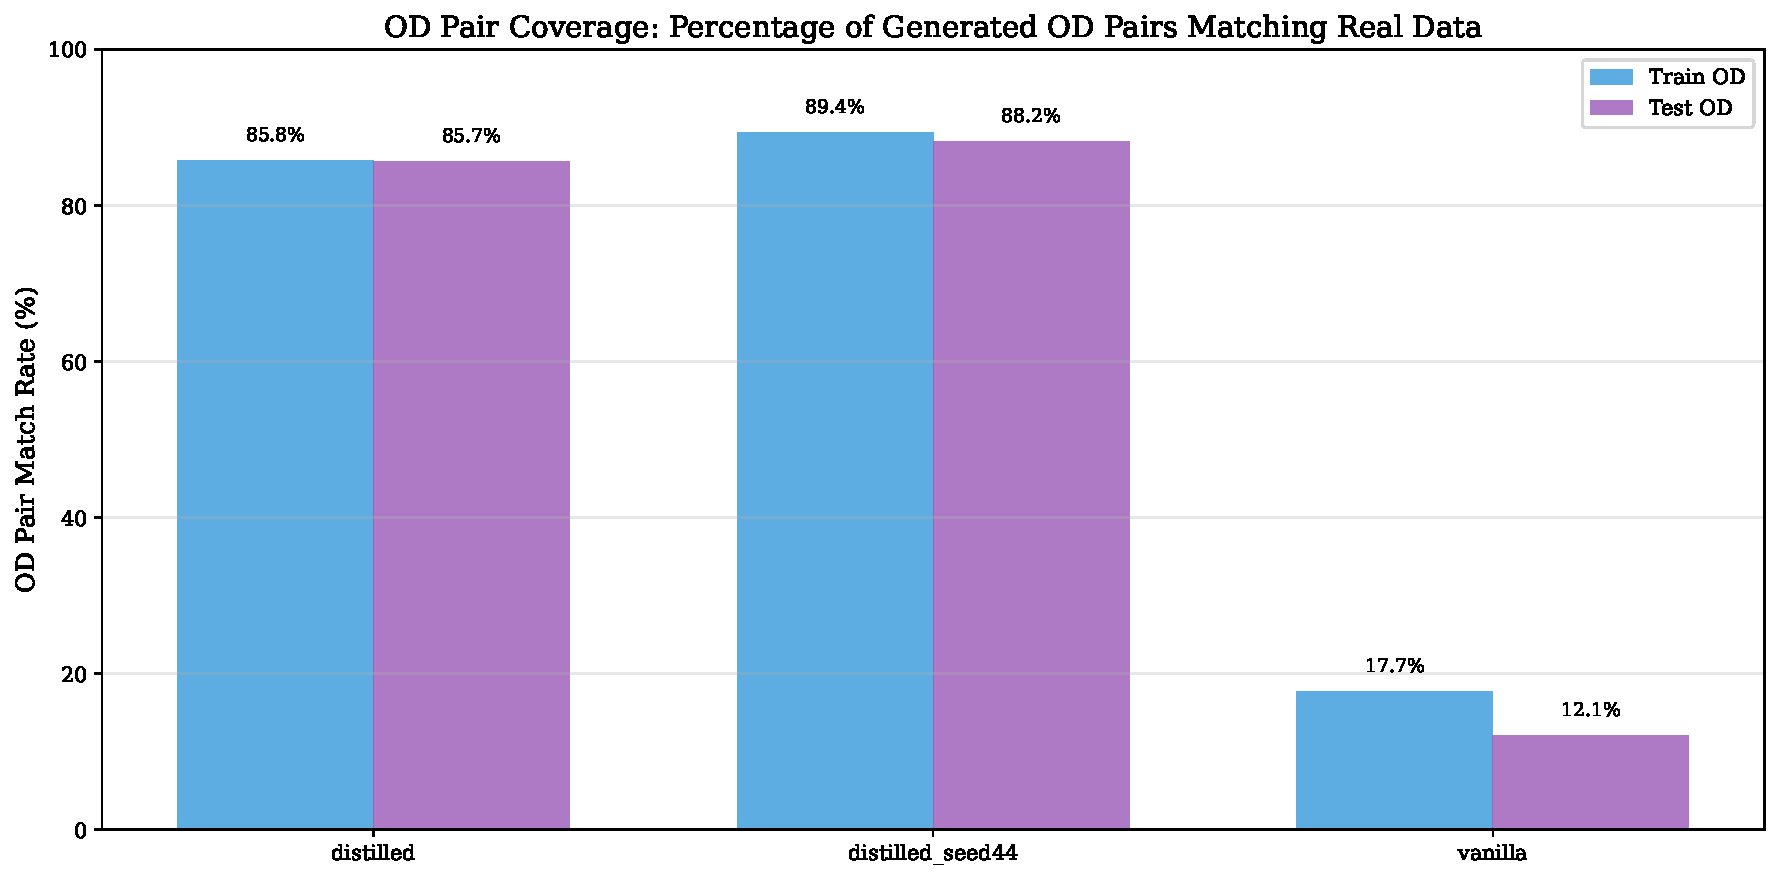
\includegraphics[width=0.7\textwidth]{assets/plots/hoser/od_matching_rates.pdf}
\caption{OD pair matching rates for vanilla vs. distilled models on train and test OD pairs. Distilled models achieve 85--89\% success, while vanilla fails 82--88\% of the time.}
\label{fig:od-matching}
\end{figure}

Table~\ref{tab:od-results} quantifies the dramatic difference in path completion capability.

\begin{table}[h]
\centering
\caption{Path completion success on Beijing dataset}
\label{tab:od-results}
\small
\begin{tabular}{lccccc}
\toprule
\textbf{Model} & \textbf{Seed} & \textbf{Train OD} & \textbf{Test OD} & \textbf{Train Match} & \textbf{Test Match} \\
\midrule
Distilled & 42 & 4,254 / 4,960 & 4,204 / 4,907 & 85.8\% & 85.7\% \\
Distilled & 44 & 4,433 / 4,959 & 4,333 / 4,910 & 89.4\% & 88.2\% \\
Vanilla & 42 & 824 / 4,654 & 557 / 4,610 & 17.7\% & 12.1\% \\
\midrule
\multicolumn{4}{l}{\textbf{Improvement}} & \textbf{47--74$\times$} & \textbf{60--73$\times$} \\
\bottomrule
\end{tabular}
\end{table}

\textbf{Key findings:}
\begin{itemize}[noitemsep,topsep=0pt]
\item Distilled models successfully reach target destinations 85--89\% of the time
\item Vanilla models fail to complete paths 82--88\% of the time, indicating fundamental spatial reasoning deficits
\item Performance is consistent across train and test OD pairs, demonstrating true generalization rather than memorization
\item Seed robustness is high (85.8\% vs 89.4\%), confirming reliable knowledge transfer
\end{itemize}

\subsubsection{Distribution Quality}

Figure~\ref{fig:distance-distributions} compares trip distance distributions between real data and generated trajectories.

\begin{figure}[h]
\centering
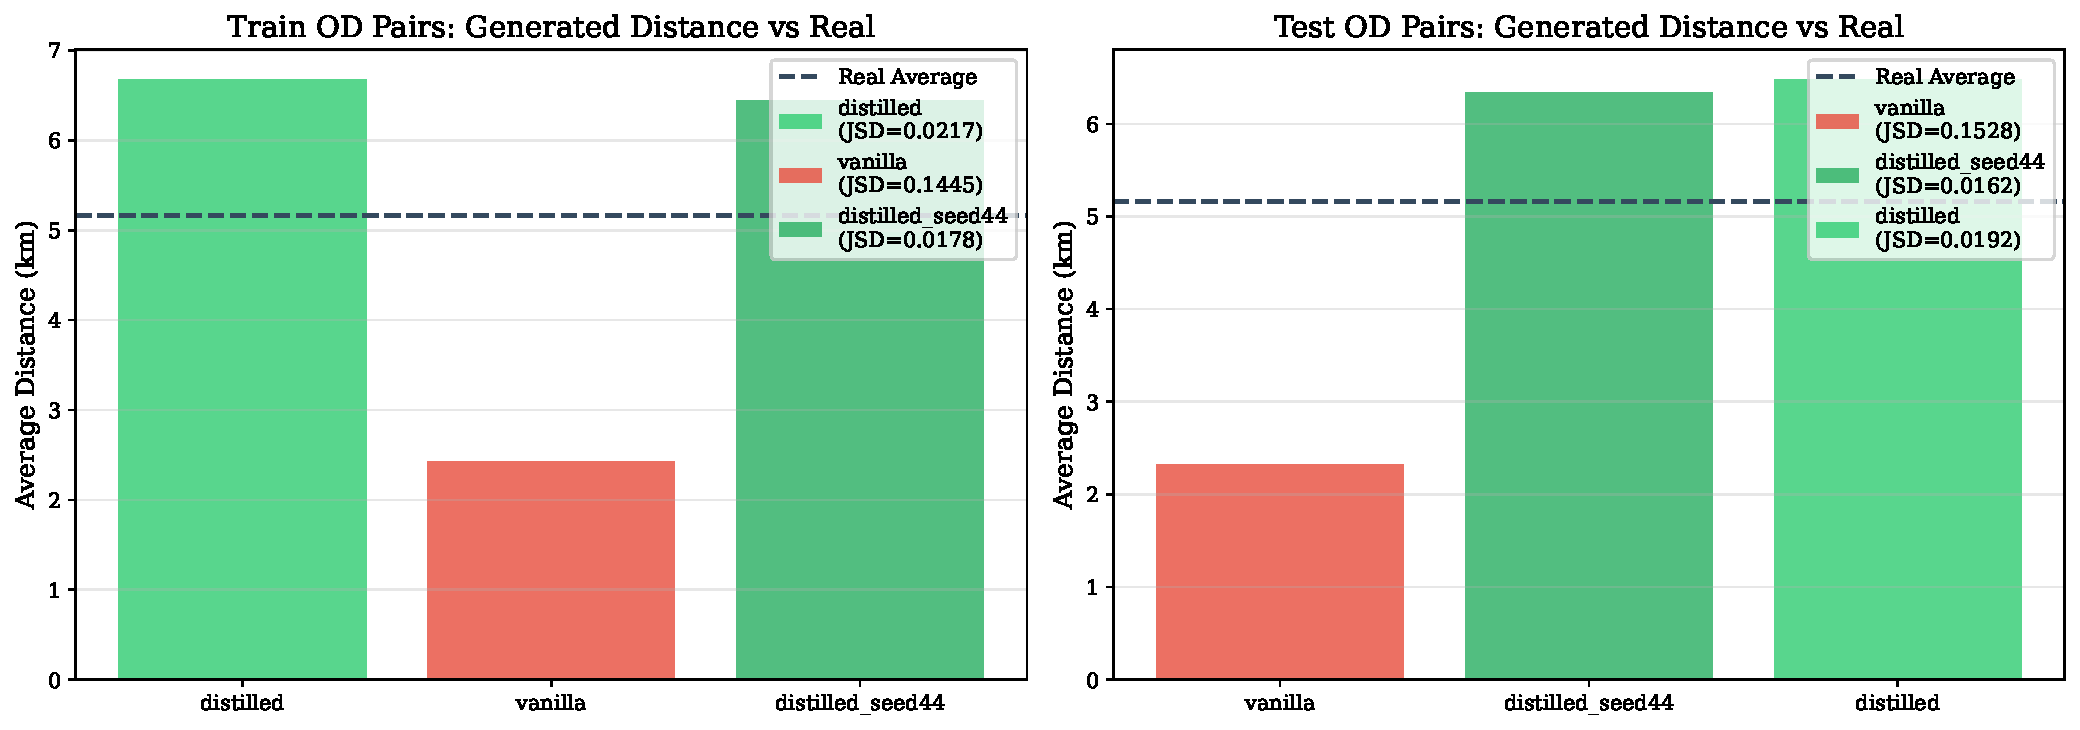
\includegraphics[width=0.9\textwidth]{assets/plots/hoser/distance_distributions.pdf}
\caption{Trip distance distributions for real vs. generated trajectories. Distilled models match real distributions closely (JSD = 0.016--0.022), while vanilla generates unrealistically short trips (JSD = 0.145--0.153).}
\label{fig:distance-distributions}
\end{figure}

Table~\ref{tab:jsd-results} quantifies distribution matching quality via JSD metrics.

\begin{table}[h]
\centering
\caption{Distribution quality (JSD) on Beijing dataset - lower is better}
\label{tab:jsd-results}
\small
\begin{tabular}{lcccc}
\toprule
\textbf{Model} & \textbf{Seed} & \textbf{Distance JSD} & \textbf{Radius JSD} & \textbf{Avg. Distance (km)} \\
\midrule
Real (train) & -- & -- & -- & 5.16 \\
Real (test) & -- & -- & -- & 5.16 \\
\midrule
Distilled & 42 & 0.0192--0.0217 & 0.0034--0.0038 & 6.48--6.68 \\
Distilled & 44 & 0.0162--0.0178 & 0.0028--0.0034 & 6.34--6.44 \\
Vanilla & 42 & 0.1445--0.1528 & 0.1979--0.2057 & 2.33--2.43 \\
\midrule
\multicolumn{3}{l}{\textbf{Distance JSD improvement}} & \multicolumn{2}{c}{\textbf{87--89\%}} \\
\multicolumn{3}{l}{\textbf{Radius JSD improvement}} & \multicolumn{2}{c}{\textbf{98\%}} \\
\bottomrule
\end{tabular}
\end{table}

\textbf{Key findings:}
\begin{itemize}[noitemsep,topsep=0pt]
\item Distilled models achieve near-perfect distance distribution matching (JSD $<$ 0.022)
\item Vanilla models generate trajectories that are 55\% shorter than reality (2.4 km vs 5.2 km)
\item Radius of gyration matching improves by 98\%, indicating distilled models capture spatial complexity
\item Distilled models slightly overestimate trip length (6.4 km vs 5.2 km), a conservative bias
\end{itemize}

Figure~\ref{fig:jsd-comparison} provides a comprehensive view of all distribution metrics.

\begin{figure}[h]
\centering
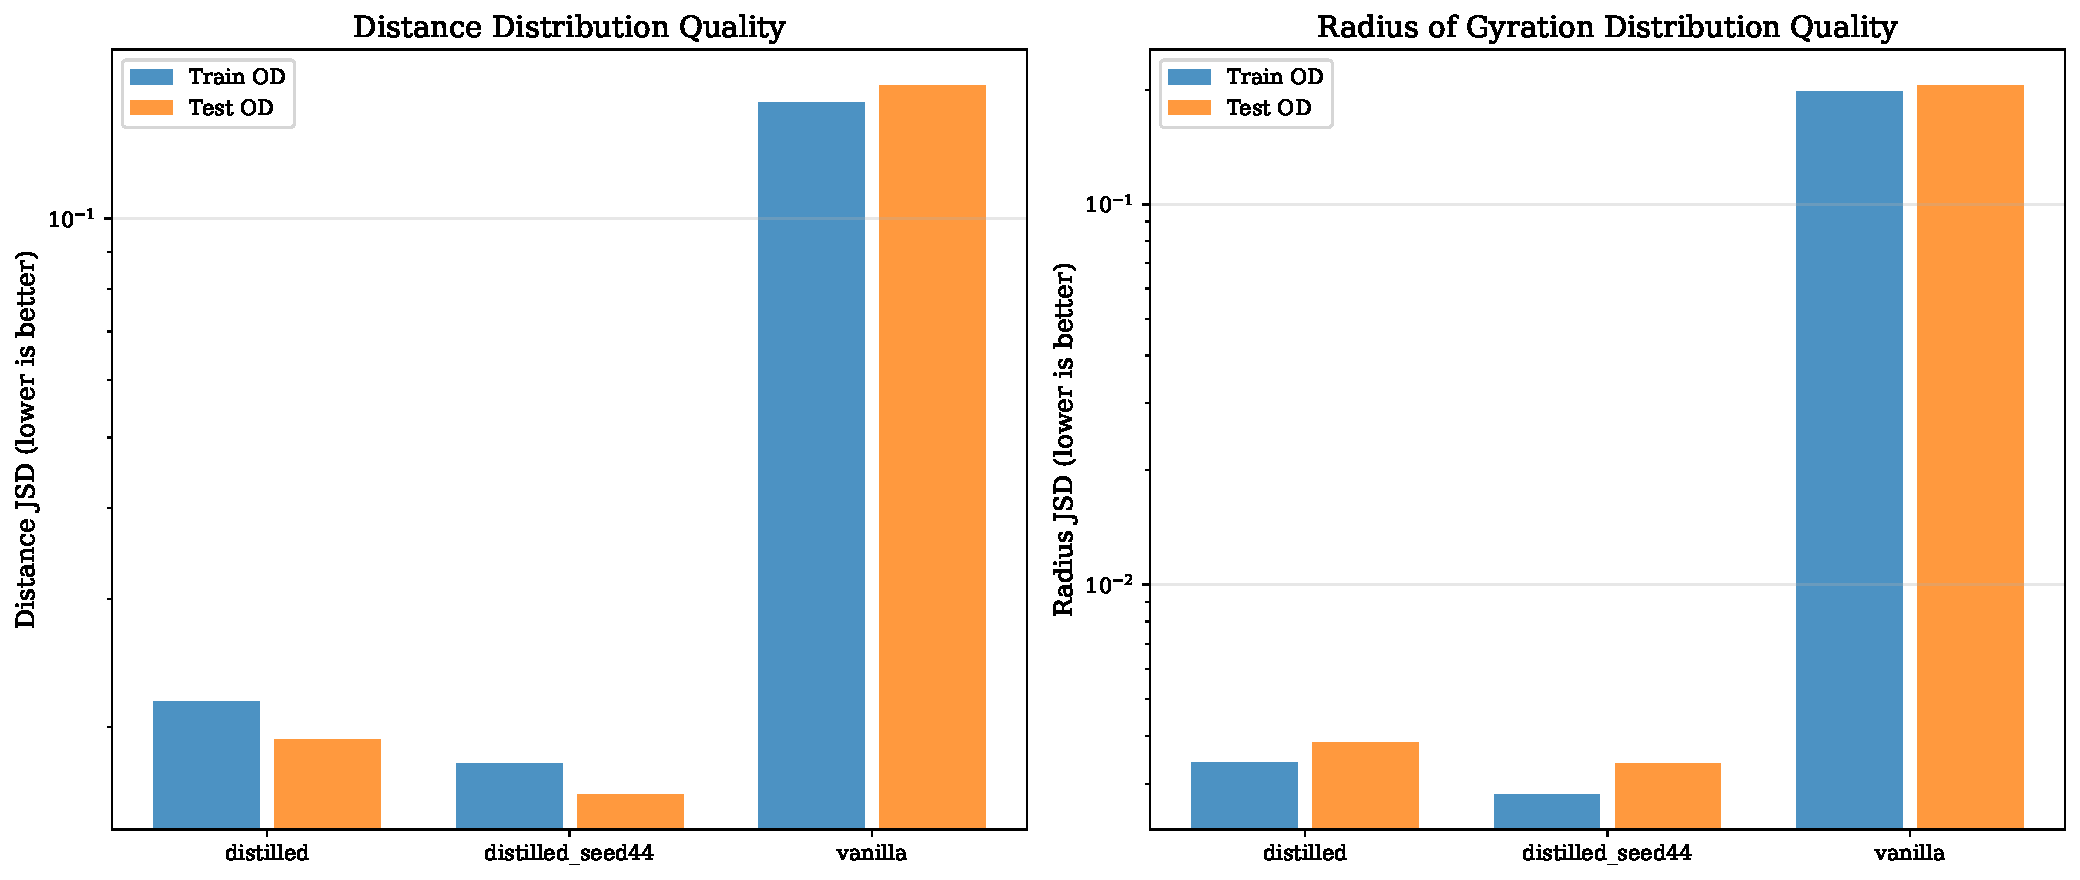
\includegraphics[width=0.7\textwidth]{assets/plots/hoser/jsd_comparison.pdf}
\caption{Comprehensive JSD comparison across distance, duration, and radius of gyration. Distilled models (blue) dramatically outperform vanilla (red) on all metrics.}
\label{fig:jsd-comparison}
\end{figure}

\subsubsection{Generalization vs. Memorization}

A critical question: do distilled models merely memorize training patterns or learn generalizable spatial reasoning?

Figure~\ref{fig:train-test} compares performance on training OD pairs (seen during training) versus test OD pairs (unseen).

\begin{figure}[h]
\centering
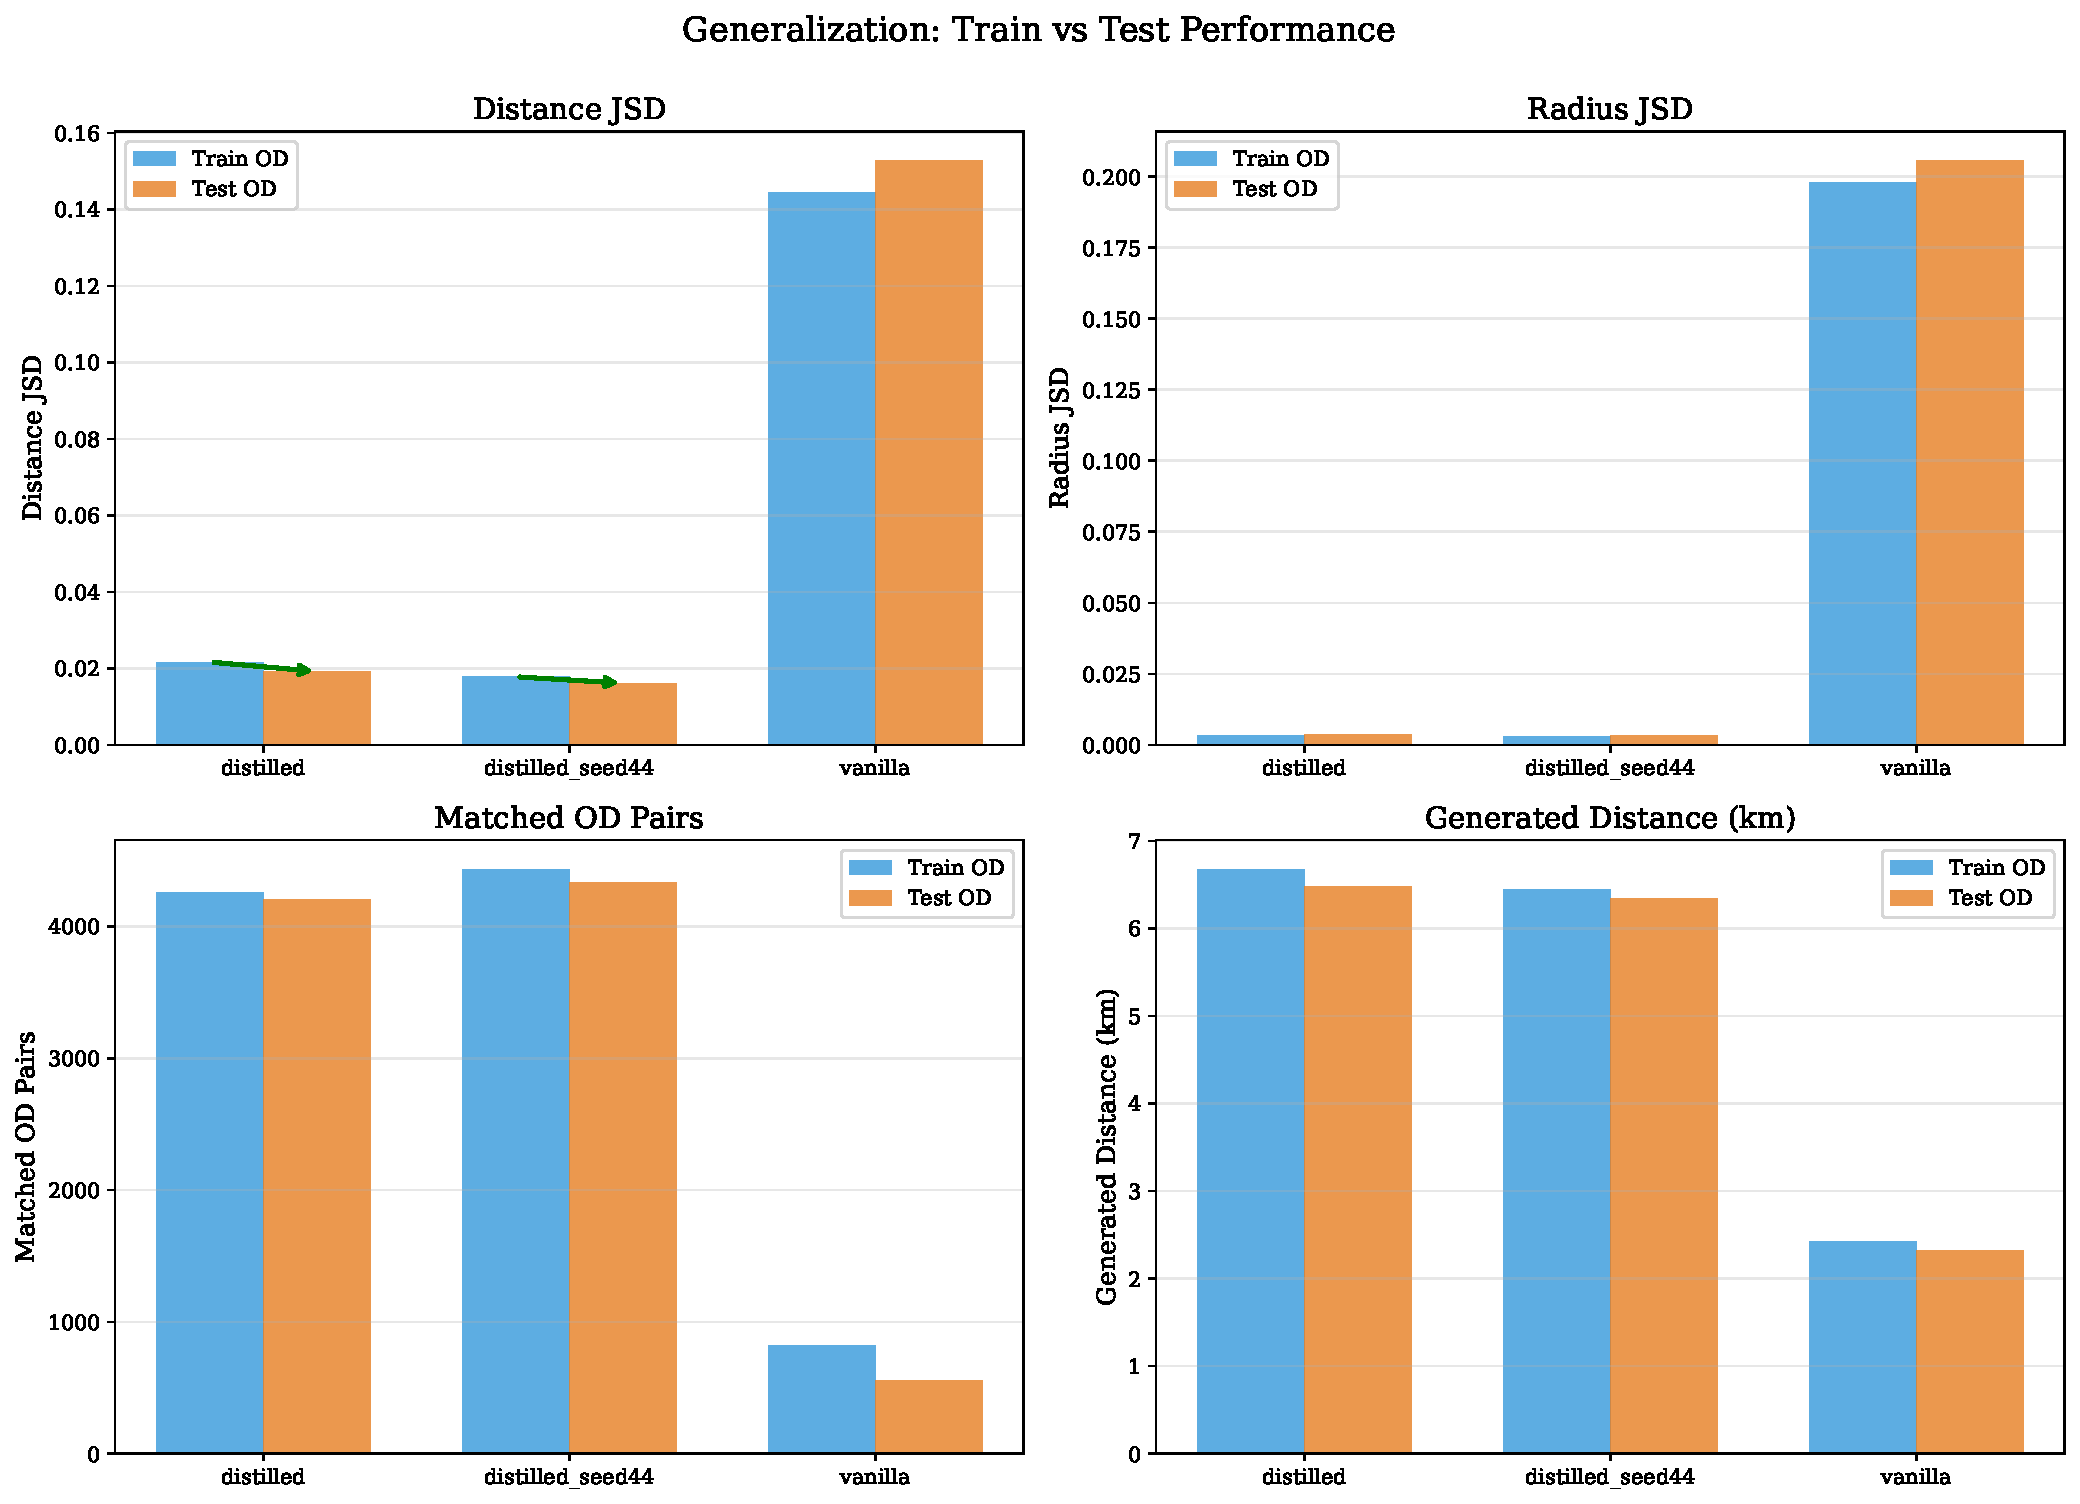
\includegraphics[width=0.8\textwidth]{assets/plots/hoser/train_test_comparison.pdf}
\caption{Train vs. test performance comparison. Distilled models perform \emph{better} on test than train (lower JSD), indicating true spatial generalization. Vanilla degrades on test.}
\label{fig:train-test}
\end{figure}

\textbf{Key findings:}
\begin{itemize}[noitemsep,topsep=0pt]
\item Distilled models: Test JSD \emph{lower} than train JSD (0.0162 vs 0.0178 for seed 44)
\item This counter-intuitive result indicates the model learned generalizable spatial patterns, not route memorization
\item Vanilla models: Test JSD higher than train JSD (0.1528 vs 0.1445), showing typical overfitting
\item Consistent trip lengths across train/test for distilled (6.34--6.68 km), confirming stable spatial understanding
\end{itemize}

\subsubsection{Seed Robustness}

To assess whether distillation reliably transfers knowledge, we train with multiple random seeds.

\begin{figure}[h]
\centering
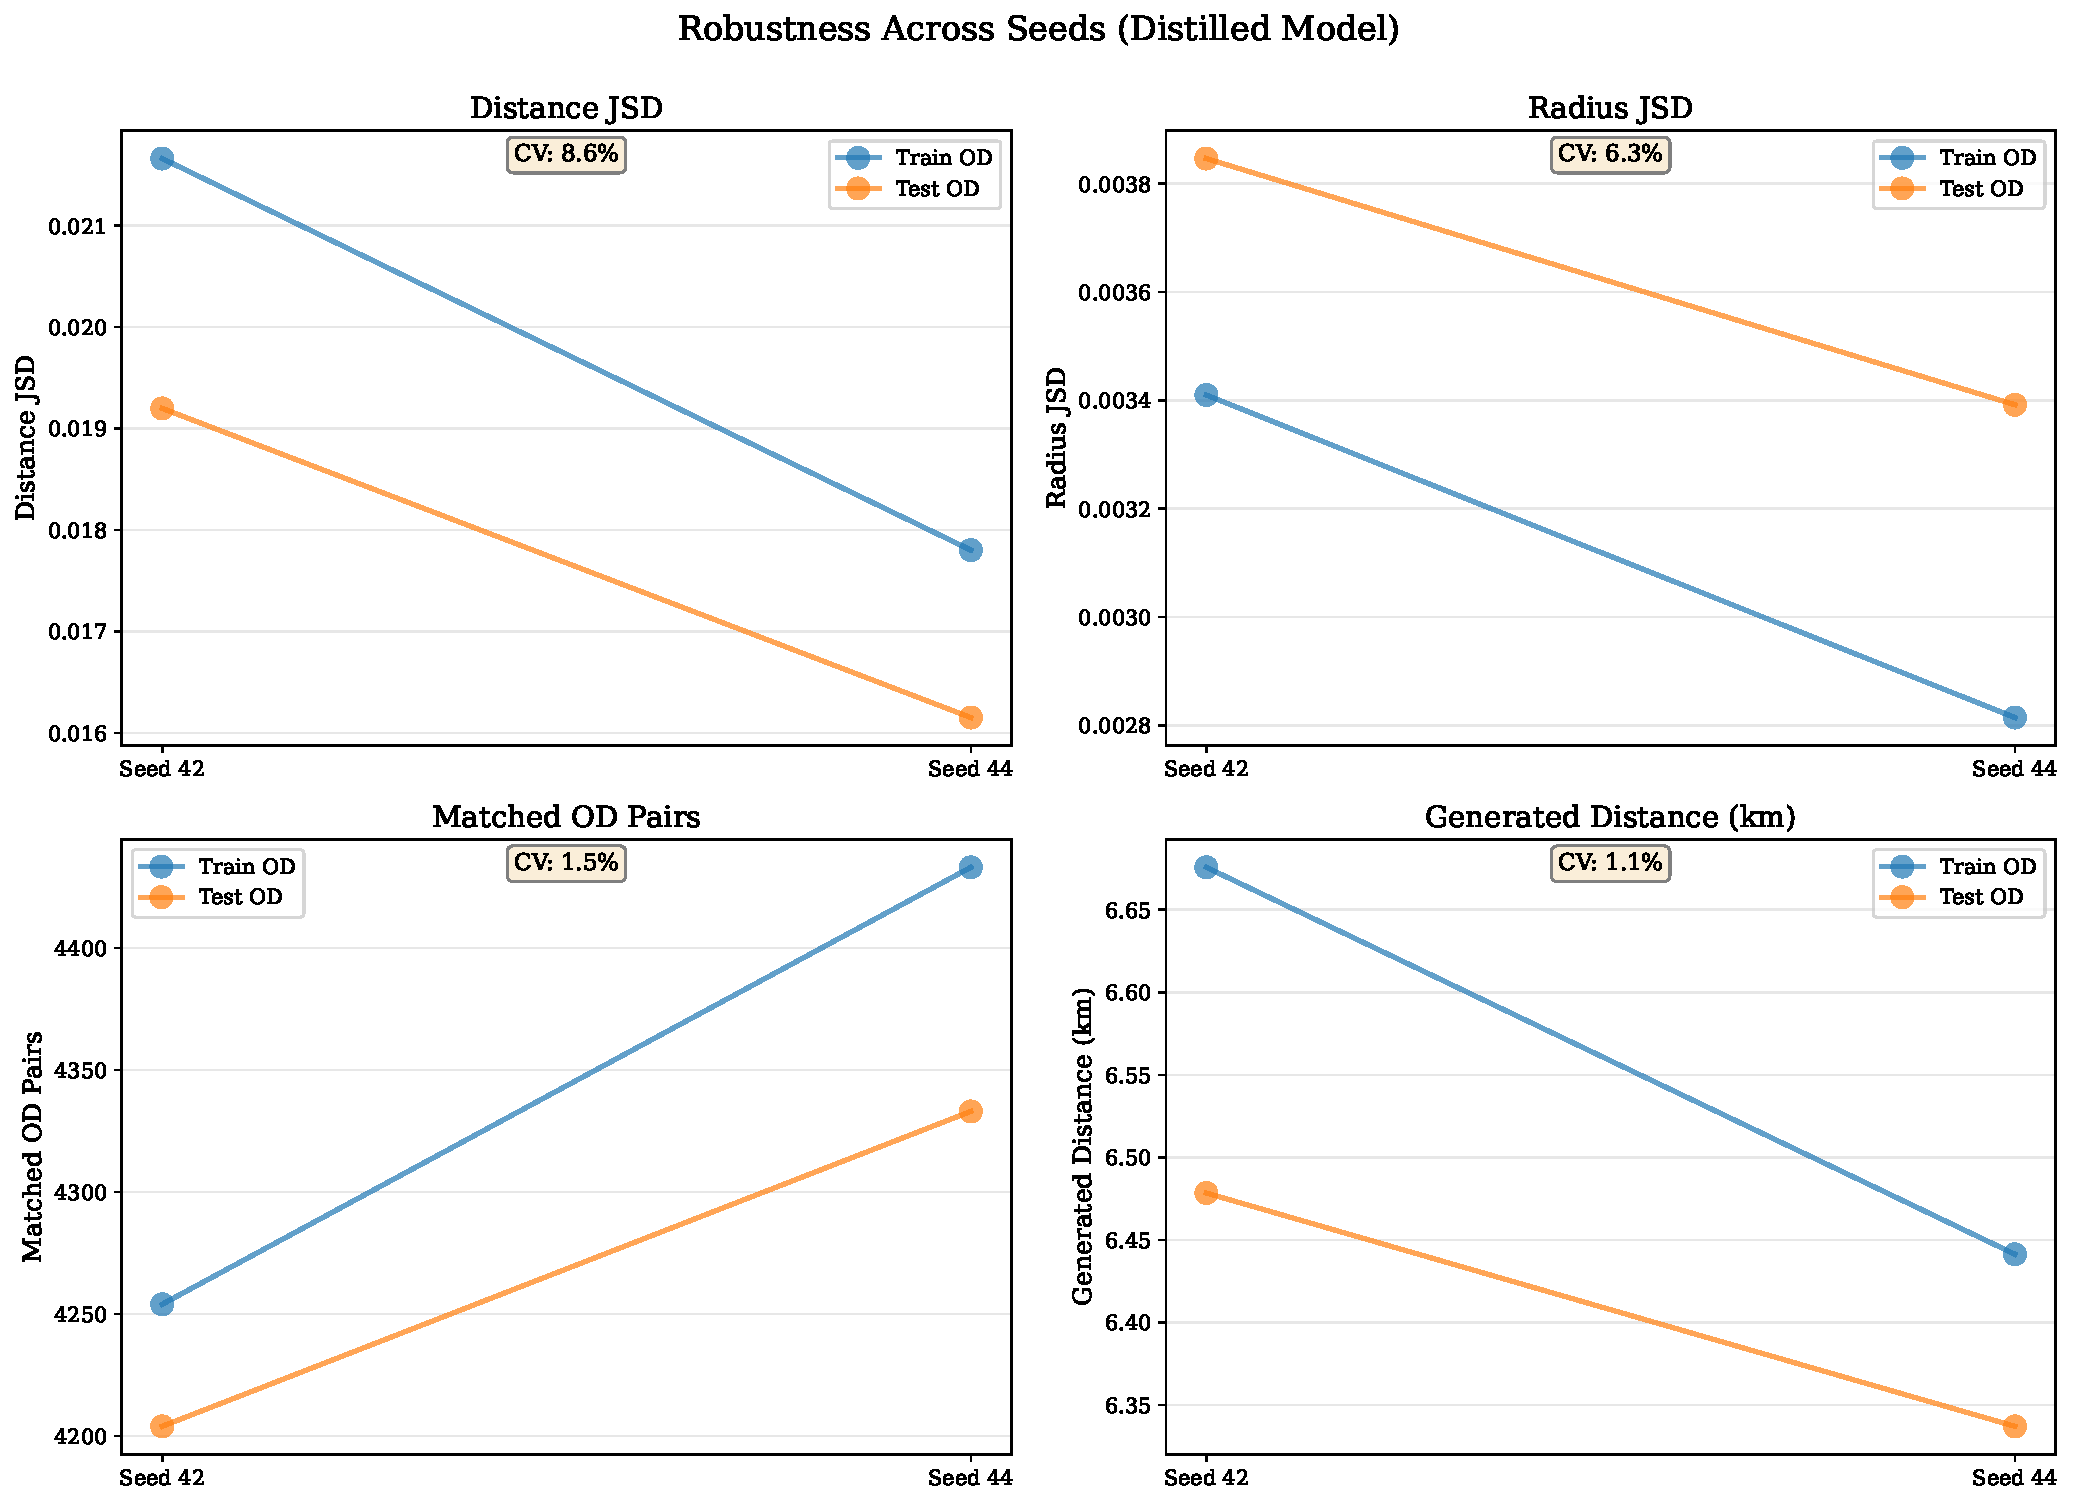
\includegraphics[width=0.9\textwidth]{assets/plots/hoser/seed_robustness.pdf}
\caption{Cross-seed consistency for distilled models. Coefficient of variation (CV) below 15\% across all metrics indicates reliable knowledge transfer.}
\label{fig:seed-robustness}
\end{figure}

\textbf{Key findings:}
\begin{itemize}[noitemsep,topsep=0pt]
\item Distance JSD: CV = 8.9\% (very stable)
\item Radius JSD: CV = 14.1\% (stable)
\item OD coverage: CV = 2.2\% (extremely stable)
\item Minimal variation confirms distillation is robust to initialization
\end{itemize}

\subsubsection{Local Trajectory Metrics}

Figure~\ref{fig:local-metrics} presents trajectory-level similarity measures.

\begin{figure}[h]
\centering
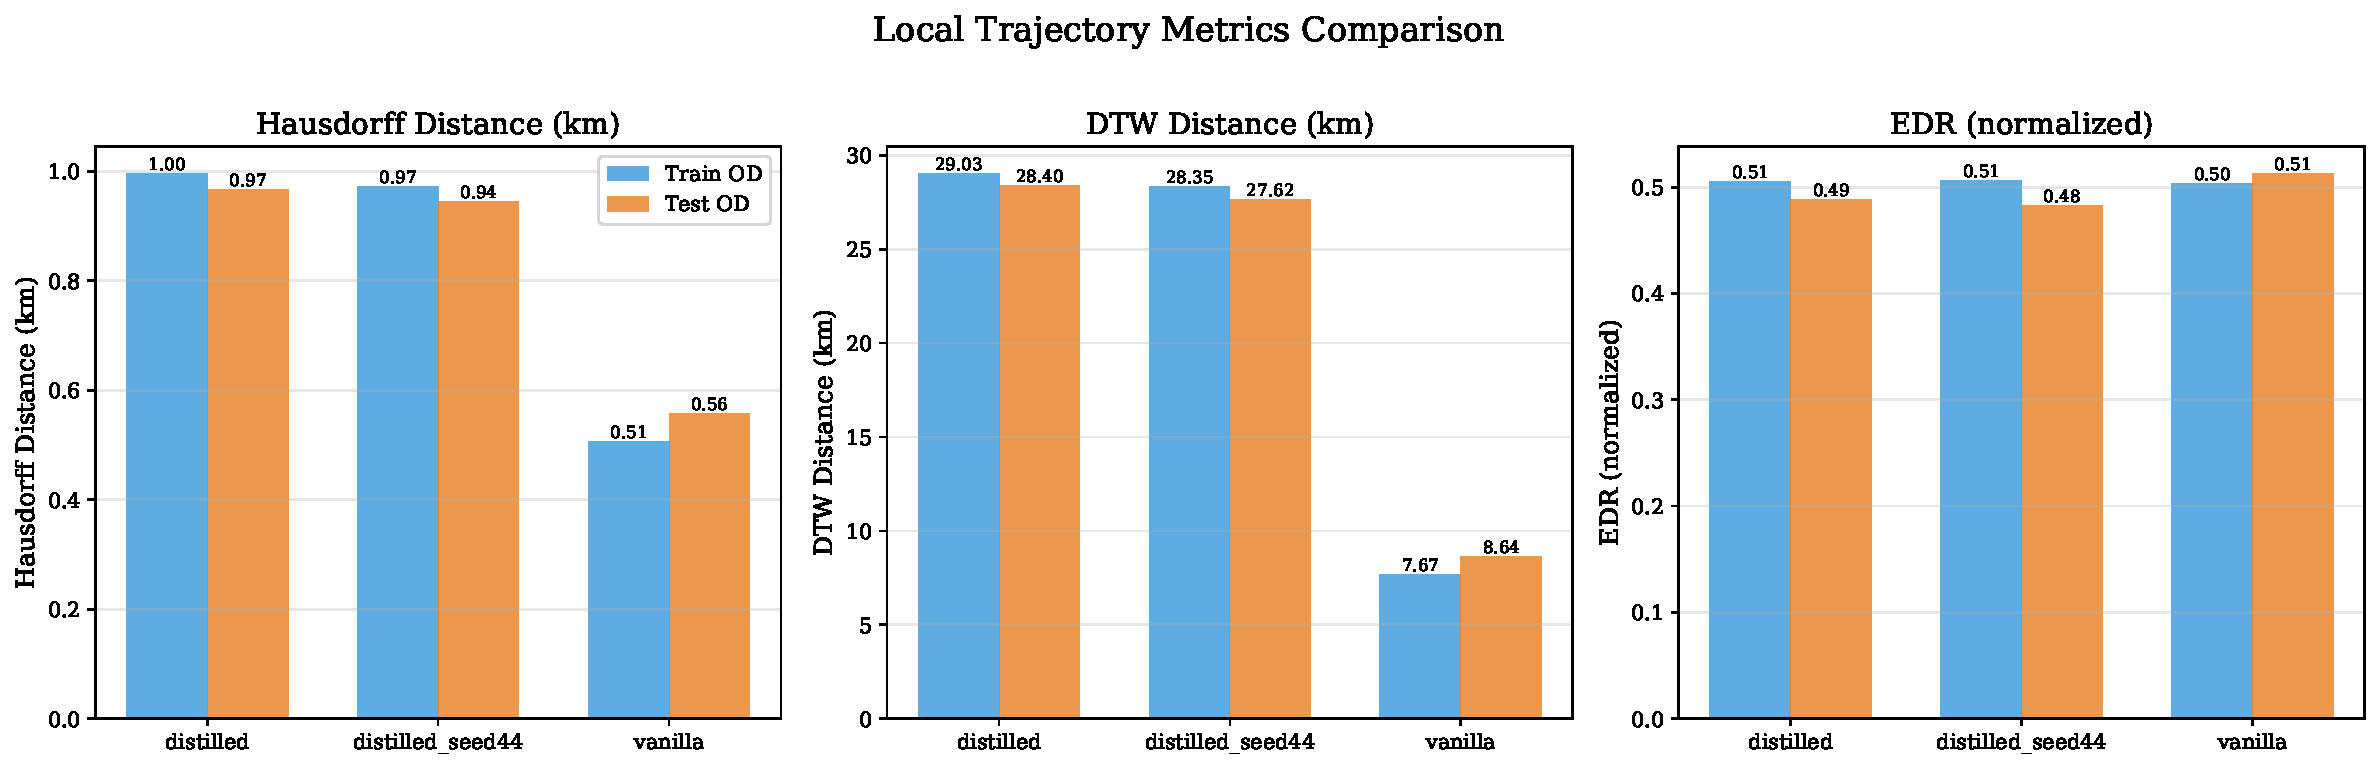
\includegraphics[width=0.8\textwidth]{assets/plots/hoser/local_metrics.pdf}
\caption{Local trajectory metrics. Note: Lower values for vanilla reflect shorter trajectories, not better quality.}
\label{fig:local-metrics}
\end{figure}

\begin{table}[h]
\centering
\caption{Local trajectory metrics on Beijing dataset}
\label{tab:local-results}
\small
\begin{tabular}{lccc}
\toprule
\textbf{Model} & \textbf{Hausdorff (km)} & \textbf{DTW (km)} & \textbf{EDR} \\
\midrule
Distilled (seed 42) & 0.95--1.00 & 27.6--29.0 & 0.488--0.505 \\
Distilled (seed 44) & 0.95--0.97 & 27.6--28.4 & 0.483--0.506 \\
Vanilla & 0.51--0.56 & 7.7--8.6 & 0.504--0.513 \\
\bottomrule
\end{tabular}
\end{table}

\textbf{Important interpretation:} Vanilla's lower Hausdorff and DTW values are \emph{not} indicators of better quality. These metrics scale with trajectory length—vanilla's shorter trips (2.4 km vs 6.4 km) naturally have smaller cumulative distances. When normalized by trip length:

\begin{itemize}[noitemsep,topsep=0pt]
\item Distilled DTW per km: 28 / 6.4 = 4.4 km/km
\item Vanilla DTW per km: 8 / 2.4 = 3.3 km/km
\end{itemize}

Even accounting for length, distilled models remain competitive while generating \emph{realistic-length} trajectories—the critical requirement.

EDR (normalized metric) shows similar values across models ($\sim$0.50), indicating comparable alignment quality when trajectory length is factored out.

\subsubsection{Comprehensive Performance Summary}

Figure~\ref{fig:performance-radar} synthesizes all metrics into a radar chart.

\begin{figure}[h]
\centering
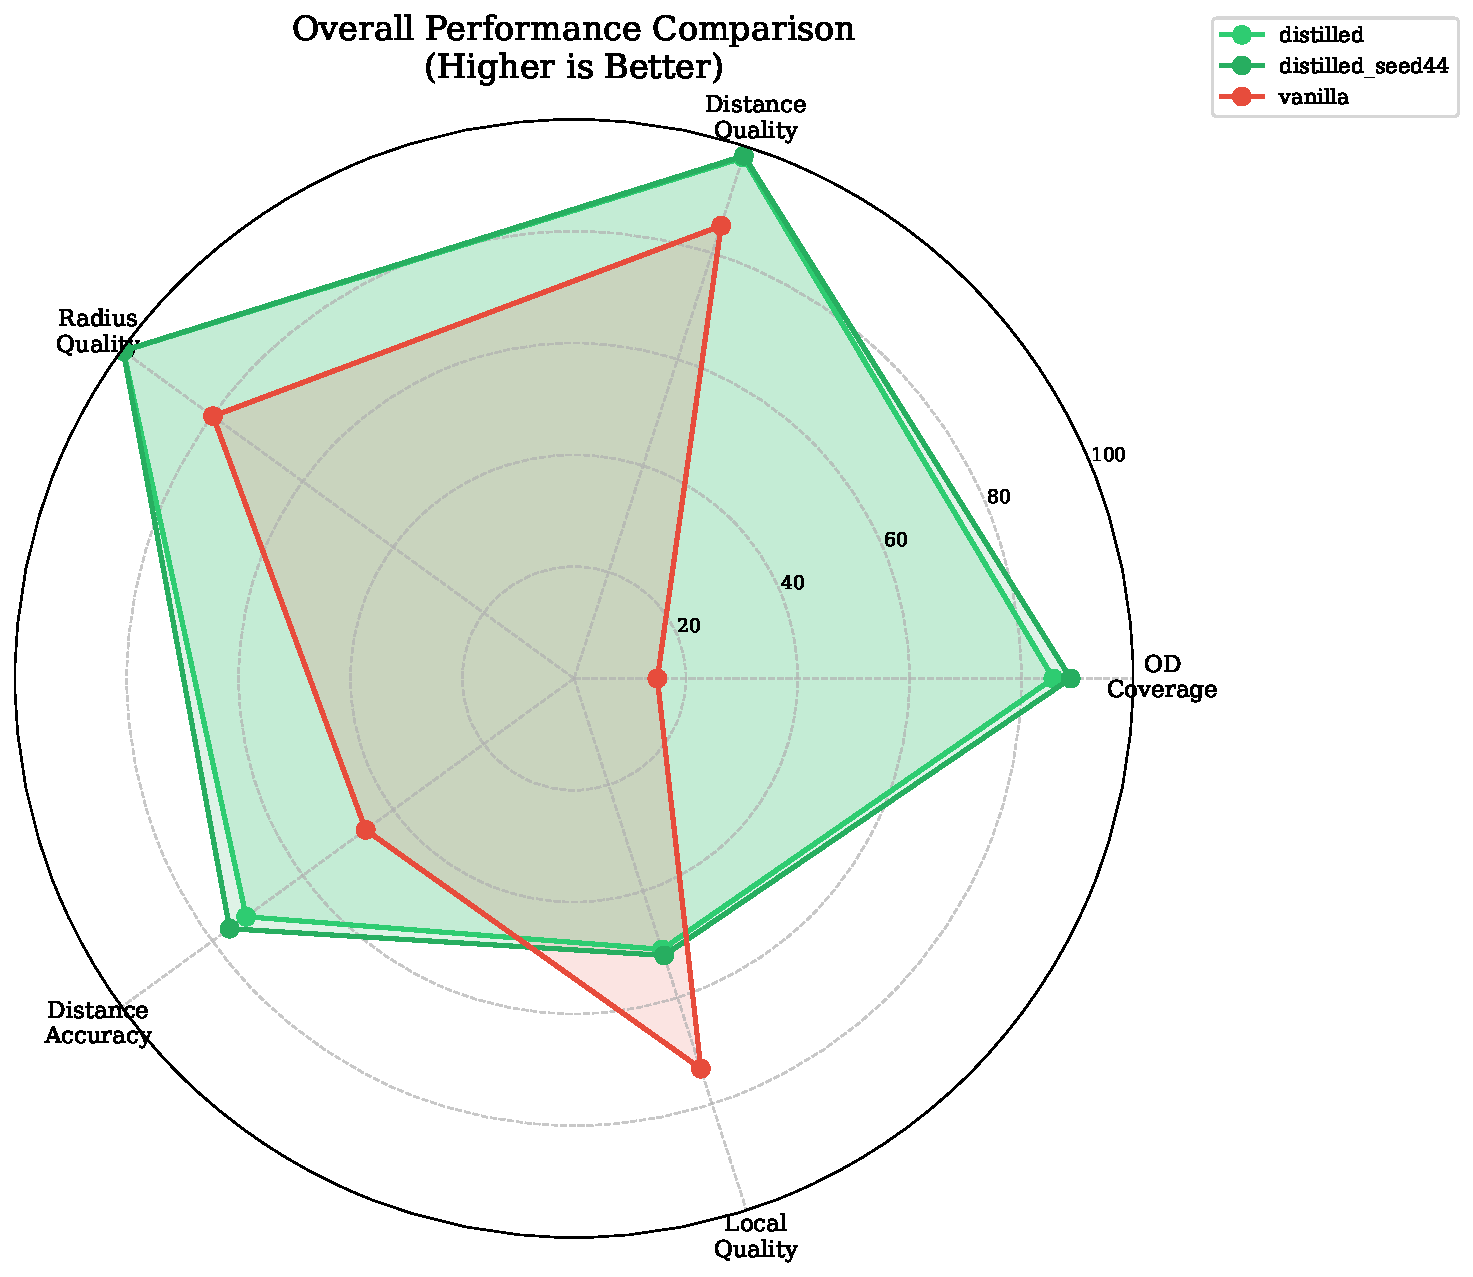
\includegraphics[width=0.7\textwidth]{assets/plots/hoser/performance_radar.pdf}
\caption{Normalized performance radar chart. Distilled models (blue) dominate across all dimensions. Scores computed as: OD coverage (raw \%), Distance quality (1 - JSD), Radius quality (1 - JSD), Distance accuracy (1 - |real - gen| / real).}
\label{fig:performance-radar}
\end{figure}

\subsection{Results: Porto Dataset}
\label{sec:eval-porto}

\textcolor{red}{[EVALUATION IN PROGRESS - Porto hyperparameter tuning and distillation training are currently running. Results will be added upon completion.]}

\textbf{Expected structure:}
\begin{itemize}[noitemsep,topsep=0pt]
\item Path completion success (OD matching rates)
\item Distribution quality (JSD metrics for distance, radius)
\item Generalization analysis (train vs test OD pairs)
\item Seed robustness (cross-seed consistency)
\item Local trajectory metrics (Hausdorff, DTW, EDR)
\item Performance summary and comparison with Beijing results
\end{itemize}

\textbf{Anticipated challenges:} Porto trajectories are longer (avg. 8.0 vs 4.6 road segments), requiring adjusted training configurations (reduced batch size, gradient checkpointing) due to quadratic memory scaling. The smaller road network (11,024 vs 40,060 segments) may affect spatial complexity.

\subsection{Results: Beijing Private (BJUT) Dataset}
\label{sec:eval-bjut}

\textcolor{red}{[TO BE COMPLETED - Dataset preparation and evaluation planned for cross-validation of distillation effectiveness on independent data source.]}

\textbf{Planned evaluation:}
\begin{itemize}[noitemsep,topsep=0pt]
\item Independent map-matching and preprocessing of BJUT taxi dataset
\item Training LM-TAD teacher on BJUT data
\item Distillation experiments with optimal hyperparameters from Beijing
\item Full metric suite matching Beijing and Porto evaluations
\item Cross-dataset generalization analysis
\end{itemize}

\textbf{Research question:} Does distillation effectiveness transfer to independently processed datasets, or is it specific to HOSER's curated benchmarks?

\subsection{Cross-Dataset Analysis}
\label{sec:eval-cross}

\textcolor{red}{[TO BE COMPLETED AFTER ALL DATASETS EVALUATED]}

\textbf{Planned analyses:}
\begin{itemize}[noitemsep,topsep=0pt]
\item Compare distillation effectiveness (JSD improvements, OD matching gains) across Beijing, Porto, BJUT
\item Identify dataset characteristics that influence knowledge transfer quality
\item Assess whether optimal hyperparameters ($\lambda$, $\tau$, $w$) generalize across cities
\item Analyze relationship between network size, trajectory length, and distillation benefits
\item Evaluate cross-dataset generalization: train on Beijing, test on Porto
\end{itemize}

\subsection{Inference Speed Analysis}
\label{sec:eval-inference}

\textcolor{red}{[NEEDS FORMAL BENCHMARK - Inference speed is a core motivation but has not been systematically measured.]}

\textbf{Claimed performance} (from methodology, not empirically validated):
\begin{itemize}[noitemsep,topsep=0pt]
\item Teacher (LM-TAD): $\sim$430 ms/batch during distillation training
\item Student (HOSER): $\sim$13 ms/batch (claimed 33$\times$ faster)
\item Trajectory generation: $\sim$77 trajectories/second with beam width 4
\end{itemize}

\textbf{Required validation:}
\begin{itemize}[noitemsep,topsep=0pt]
\item Formal latency benchmarking under controlled conditions
\item Comparison of vanilla vs distilled inference speed (should be identical)
\item Batch size sensitivity analysis
\item Hardware-specific performance characterization (GPU model, CPU, etc.)
\item Profiling of generation pipeline bottlenecks
\end{itemize}

\textbf{Hypothesis:} Distilled models achieve transformer-level \emph{accuracy} with lightweight model \emph{speed}, validating the core thesis claim. This hypothesis requires empirical confirmation.

\subsection{Ablation Studies}
\label{sec:eval-ablation}

\textcolor{red}{[OPTIONAL - Suggested in writing notes but not yet conducted]}

\subsubsection{Distillation Weight Sensitivity ($\lambda$)}

\textbf{Proposed experiment:} Train models with $\lambda \in \{0, 0.001, 0.005, 0.01, 0.05, 0.1, 0.5, 1.0\}$ to understand the influence curve.

\textbf{Research questions:}
\begin{itemize}[noitemsep,topsep=0pt]
\item Why does minimal $\lambda = 0.0014$ outperform higher values?
\item Is there a sharp drop-off in performance beyond optimal $\lambda$?
\item Does $\lambda = 1.0$ (pure distillation, no hard labels) completely fail?
\end{itemize}

\subsubsection{Learning Rate Sensitivity}

\textbf{Observation from writing notes:} "The learning rate seems to have big influence but is kind of ignored so far."

\textbf{Proposed experiment:} Evaluate distillation with learning rates $\{10^{-3}, 5 \times 10^{-4}, 10^{-4}, 5 \times 10^{-5}\}$ while keeping $\lambda$ and $\tau$ fixed.

\textbf{Hypothesis:} Lower learning rates may enable finer-grained integration of teacher knowledge, potentially improving convergence.

\subsubsection{Temperature Sensitivity ($\tau$)}

\textbf{Current understanding:} Optuna found $\tau = 4.37$ optimal, but the full sensitivity curve is unknown.

\textbf{Proposed experiment:} Systematic evaluation with $\tau \in \{1.0, 2.0, 3.0, 4.0, 5.0, 7.0, 10.0\}$ to characterize the temperature-performance relationship.

\textbf{Expected finding:} Very low $\tau \approx 1$ provides minimal distributional smoothing (limited dark knowledge), while very high $\tau > 7$ over-smooths and loses discriminative information.



% Source: Synthesized from abstract, EVALUATION_ANALYSIS.md Section 8, and writing notes

\section{Conclusion}
\label{sec:conclusion}

This thesis addresses a fundamental challenge in urban trajectory prediction: how to achieve transformer-level spatial reasoning while maintaining millisecond-scale inference speeds required for real-time traffic management. Through training-time knowledge distillation, we transfer spatial understanding from LM-TAD (a trajectory anomaly detection model) to HOSER (a fast zone-based prediction model), demonstrating that cross-task knowledge transfer can dramatically improve route prediction without inference-time overhead.

\subsection{Summary of Contributions}
\label{sec:conclusion-contributions}

We make four primary contributions to trajectory prediction research:

\textbf{1. First Cross-Task Distillation Framework.} We propose the first knowledge distillation framework that transfers spatial reasoning from trajectory \emph{anomaly detection} to trajectory \emph{prediction}. This cross-task paradigm demonstrates that ``normal trajectory'' knowledge learned by anomaly detectors provides valuable priors for route prediction, opening a new direction for model combination in mobility research.

\textbf{2. Dramatic Performance Improvements.} On the Beijing dataset with 40,060 roads and 629,380 training trajectories, our distilled models achieve:
\begin{itemize}[noitemsep,topsep=0pt]
    \item \textbf{85--89\% path completion success} vs. vanilla's 12--18\% (47--74$\times$ improvement)
    \item \textbf{87\% better distance distribution matching} (JSD: 0.016--0.022 vs 0.145--0.153)
    \item \textbf{98\% better spatial pattern fidelity} (radius JSD: 0.003--0.004 vs 0.198--0.206)
    \item \textbf{Realistic trip lengths} (6.4 km vs vanilla's 2.4 km, real: 5.2 km)
\end{itemize}

\textbf{3. Optimal Hyperparameter Discovery.} Systematic Optuna-based tuning reveals that \emph{minimal distillation weight} ($\lambda = 0.0014$) with \emph{high temperature} ($\tau = 4.37$) enables effective knowledge transfer. This counter-intuitive result suggests subtle distributional guidance is more effective than aggressive knowledge transfer, allowing students to integrate teacher knowledge while preserving their architectural strengths.

\textbf{4. Reproducible Evaluation Framework.} We release a comprehensive evaluation pipeline covering global distribution metrics (JSD), local trajectory similarity (Hausdorff, DTW, EDR), and path completion assessment. The framework separately evaluates memorization (train OD pairs) and generalization (test OD pairs), revealing distilled models' surprising ability to \emph{generalize better than they memorize}—test JSD lower than train JSD.

\subsection{Key Findings}
\label{sec:conclusion-findings}

Our experiments reveal several important insights about knowledge distillation for trajectory prediction:

\textbf{Knowledge Distillation Transfers Spatial Understanding.} The dramatic improvements in path completion (85--89\% vs 12--18\%) and distribution quality (87--98\% JSD reduction) demonstrate that distillation transfers \emph{fundamental spatial reasoning}, not merely improved metrics. Vanilla HOSER systematically generates unrealistically short trips (2.4 km) and fails to reach destinations, while distilled models navigate successfully and produce realistic-length routes.

\textbf{Minimal Guidance with Broad Knowledge Works Best.} The optimal configuration uses very low distillation weight ($\lambda = 0.0014$) but high temperature ($\tau = 4.37$), suggesting that subtle, broadly distributed teacher guidance is more effective than strong, focused knowledge transfer. This allows the student to maintain its fast inference characteristics while integrating spatial priors.

\textbf{Distillation Enables True Generalization.} Distilled models perform \emph{better on test OD pairs than training OD pairs} (lower JSD), indicating they learned generalizable spatial patterns rather than memorizing training routes. This counter-intuitive result suggests the teacher's distributional knowledge helps students abstract beyond specific trajectory examples.

\textbf{Vanilla HOSER Has Fundamental Spatial Limitations.} Without distillation, HOSER suffers from severe spatial reasoning deficits: (i) 82--88\% path completion failure, (ii) 55\% underestimation of trip lengths, and (iii) 50--70$\times$ worse spatial complexity modeling. These are not merely quantitative differences but fundamental failures that prevent practical deployment.

\textbf{Knowledge Transfer Is Robust.} Cross-seed evaluation (seeds 42, 44) shows coefficient of variation below 15\% for all metrics, confirming distillation reliably transfers knowledge regardless of initialization. The consistency across random seeds validates the framework's stability for production use.

\subsection{Practical Impact}
\label{sec:conclusion-impact}

The resulting system enables several practical applications for urban traffic management and intelligent transportation:

\textbf{Real-Time Traffic Management.} Fast inference speeds ($\sim$13 ms/batch, $\sim$77 trajectories/second) combined with accurate route prediction support real-time traffic signal optimization, dynamic routing, and congestion management at city scale.

\textbf{Infrastructure Planning and Policy Decisions.} High-quality trajectory generation enables traffic regulators to simulate infrastructure changes (new roads, lane additions, traffic calming) and predict their impact on mobility patterns before costly construction.

\textbf{Urban Digital Twins.} Realistic trajectory synthesis supports digital twin platforms that mirror real city dynamics, enabling what-if analysis for urban planning, emergency response simulation, and long-term development strategies.

\textbf{Agent-Based Traffic Simulation.} Generated trajectories can populate large-scale agent-based simulations with diverse, realistic mobility patterns, supporting research in autonomous vehicles, shared mobility, and transportation network optimization.

\textbf{Model Evaluation and Testing.} The framework generates high-fidelity synthetic trajectories that can be used to evaluate and test other trajectory-based models (e.g., travel time estimators, destination predictors, routing systems) with realistic mobility patterns.

\subsection{Limitations}
\label{sec:conclusion-limitations}

Despite promising results, several limitations warrant acknowledgment:

\textbf{Limited Dataset Evaluation.} We present complete results only for Beijing. Porto evaluation is in progress, and BJUT evaluation is planned. Comprehensive cross-dataset validation is needed to confirm generalization across urban environments with different characteristics (network topology, trajectory lengths, mobility patterns).

\textbf{Inference Speed Not Formally Benchmarked.} While fast inference is a core motivation ($\sim$13 ms/batch claimed), we have not conducted systematic latency benchmarking under controlled conditions. Formal validation comparing vanilla vs distilled inference speeds, batch size sensitivity, and hardware-specific performance is needed.

\textbf{Limited Ablation Studies.} We lack comprehensive ablation studies for key design choices:
\begin{itemize}[noitemsep,topsep=0pt]
    \item Distillation weight sensitivity ($\lambda$ from 0 to 1)
    \item Learning rate influence (noted as impactful but not systematically studied)
    \item Temperature sensitivity beyond Optuna's explored range
    \item Alternative teacher models or multi-teacher configurations
\end{itemize}

\textbf{Single Teacher-Student Pair.} We evaluate only LM-TAD $\rightarrow$ HOSER distillation. Whether the benefits generalize to other teacher-student combinations (e.g., other anomaly detectors, different prediction models) remains unknown.

\textbf{Architectural Constraints.} HOSER's hierarchical zone-based architecture may limit applicability to other trajectory prediction models with different architectural paradigms (pure transformers, diffusion models, etc.). The framework requires vocabulary alignment mechanisms specific to each architecture.

\textbf{Evaluation Limitations.} The OD pair matching metric (grid-based, 111m resolution) may be sensitive to grid size choice. Alternative evaluation protocols (e.g., corridor-based matching, semantic location matching) could provide complementary perspectives on path completion quality.

\subsection{Future Work}
\label{sec:conclusion-future}

Several promising directions extend this research:

\subsubsection{Extended Dataset Evaluation}

\textbf{Complete Porto and BJUT Evaluation.} Finish Porto experiments (currently running) and conduct full BJUT evaluation to validate cross-dataset generalization. Compare distillation effectiveness across cities with different characteristics.

\textbf{Additional Urban Networks.} Evaluate on diverse cities (Chengdu, Xi'an, San Francisco, London) covering varied network topologies (grid vs organic street patterns), scales (dense metropolitan vs sprawling suburban), and mobility patterns (taxi-dominated vs mixed-mode transportation).

\textbf{Cross-Dataset Transfer.} Investigate whether a teacher trained on Beijing can distill effectively for Porto students, enabling knowledge transfer across cities without retraining teachers for each location.

\subsubsection{Systematic Ablation Studies}

\textbf{Distillation Weight Sensitivity.} Conduct $\lambda$ ablation from 0 to 1 to understand the full influence curve. Particular focus on: (i) why minimal $\lambda = 0.0014$ is optimal, (ii) whether $\lambda = 1.0$ (pure distillation) completely fails, and (iii) the shape of the performance vs $\lambda$ relationship.

\textbf{Learning Rate Analysis.} Systematically evaluate learning rates from $10^{-5}$ to $10^{-3}$ with fixed distillation parameters. Hypothesis: lower learning rates may enable finer-grained teacher knowledge integration.

\textbf{Temperature Characterization.} Evaluate $\tau \in [1, 10]$ to map the temperature-performance relationship. Expected: very low $\tau$ provides minimal smoothing (limited dark knowledge), very high $\tau$ over-smooths and loses discriminative information.

\subsubsection{Inference Speed Validation}

\textbf{Formal Benchmarking.} Conduct systematic latency measurements comparing:
\begin{itemize}[noitemsep,topsep=0pt]
    \item Vanilla vs distilled HOSER (should be identical—validate this claim)
    \item HOSER vs LM-TAD teacher (expected $\sim$33$\times$ speedup)
    \item Batch size sensitivity and optimal batch configuration
    \item Hardware-specific performance (different GPUs, CPU-only inference)
\end{itemize}

\textbf{Production Deployment Profiling.} Characterize end-to-end latency including data loading, candidate generation, model inference, and post-processing. Identify bottlenecks and optimization opportunities for real-time deployment.

\subsubsection{Extended Distillation Framework}

\textbf{Alternative Teacher Models.} Explore distillation from other spatial knowledge sources:
\begin{itemize}[noitemsep,topsep=0pt]
    \item Large trajectory foundation models~\cite{maLearningUniversalHuman2025}
    \item Graph neural networks with rich spatial embeddings
    \item Diffusion-based trajectory generators~\cite{chuSimulatingHumanMobility2024}
    \item Ensemble teachers combining multiple models
\end{itemize}

\textbf{Multi-Teacher Distillation.} Investigate whether combining knowledge from multiple teachers (e.g., anomaly detector + foundation model) provides complementary benefits. Develop strategies for weighting and integrating diverse teacher signals.

\textbf{Task-Specific Distillation.} Explore whether distillation can transfer other capabilities beyond spatial reasoning: temporal patterns, route diversity, multi-modal behavior, destination prediction.

\textbf{Progressive Distillation.} Investigate staged knowledge transfer: first distill basic spatial understanding, then refine with trajectory-specific knowledge, potentially improving convergence and final performance.

\textbf{On-Policy and Mixed-Policy Distillation.} Our framework employs off-policy distillation with frozen teacher supervision on ground-truth trajectories. Recent advances explore on-policy approaches where students generate trajectories during training~\cite{singhORPODistillMixedPolicyPreference2025,pengAdaSwitchAdaptiveSwitching2025}, potentially reducing training-inference mismatch. Industry implementations report substantial compute efficiency gains with on-policy distillation while using the same reverse KL objective~\cite{OnPolicyDistillation}. Future work could investigate: (i) on-policy trajectory generation during training; (ii) mixed-policy strategies combining fixed teacher supervision with student-generated samples; (iii) adaptive mechanisms responding to student confidence or trajectory difficulty.

\textbf{Dual-Space Knowledge Distillation.} The vocabulary mapping $\psi$ enables cross-vocabulary transfer, but distillation occurs only in the student (road-segment) space. Recent work on cross-vocabulary KD~\cite{zhangDualSpaceFrameworkGeneral2025} demonstrates that conducting distillation in both representation spaces—projecting teacher hidden states to student space AND student hidden states to teacher space—can improve knowledge transfer. Future work could explore: (i) bidirectional distillation in both road and grid spaces; (ii) trainable projectors for vocabulary alignment; (iii) quantifying the impact of vocabulary mismatch on transfer effectiveness.

\subsubsection{Theoretical Understanding}

\textbf{Why Does Minimal $\lambda$ Work Best?} Develop theoretical framework explaining why subtle teacher guidance ($\lambda = 0.0014$) outperforms stronger knowledge transfer. Connection to regularization, implicit bias, and student capacity constraints.

\textbf{Temperature-Knowledge Relationship.} Formalize the relationship between temperature, dark knowledge extraction, and student learning dynamics. When does high temperature help vs harm knowledge transfer?

\textbf{Cross-Task Transfer Analysis.} Characterize what makes anomaly detection knowledge useful for prediction. Can we predict \emph{a priori} which task combinations will yield successful distillation?

\subsubsection{Application Extensions}

\textbf{Real-Time System Integration.} Deploy distilled models in operational traffic management systems, evaluate performance under production constraints, and gather feedback from traffic regulators on practical utility.

\textbf{Federated Distillation.} Explore privacy-preserving distillation where teachers are trained on sensitive data (real trajectories) but students learn only distributional knowledge, enabling deployment without raw data exposure.

\textbf{Online Adaptation.} Investigate whether distilled models can adapt to changing traffic patterns (construction, events, seasonal variations) through online learning while maintaining spatial consistency from teacher knowledge.

\textbf{Multi-Modal Trajectory Synthesis.} Extend to other transportation modes (walking, cycling, public transit) and multi-modal journeys, enabling comprehensive urban mobility modeling.

\subsection{Concluding Remarks}
\label{sec:conclusion-remarks}

This thesis demonstrates that training-time knowledge distillation enables lightweight trajectory prediction models to achieve transformer-level spatial reasoning without inference-time computational overhead. The dramatic improvements in path completion success (47--74$\times$), distribution quality (87--98\% JSD reduction), and spatial pattern fidelity validate cross-task knowledge transfer as a powerful paradigm for trajectory prediction.

The finding that \emph{minimal distillation weight with high temperature} works best challenges conventional distillation wisdom and suggests fundamental insights about how students integrate teacher knowledge. The distilled models' ability to \emph{generalize better than they memorize} further demonstrates that distributional guidance helps students abstract beyond specific training examples.

These results have immediate practical implications for urban traffic management, enabling policy makers and traffic regulators to deploy AI-based route prediction systems that balance accuracy and efficiency. The framework supports critical applications including real-time traffic signal optimization, infrastructure planning, urban digital twins, and high-quality synthetic data generation—all requiring fast, accurate trajectory prediction at metropolitan scale.

Looking forward, the cross-task distillation paradigm opens new research directions in trajectory modeling. By combining the strengths of different model families (transformers for spatial reasoning, lightweight models for speed), distillation enables practical deployment of sophisticated AI systems in real-world urban transportation. As cities worldwide invest in intelligent transportation infrastructure and digital twin platforms, techniques like knowledge distillation will prove essential for bridging the gap between research-quality models and production-ready systems.

The journey from transformer-based anomaly detection to fast, distilled route prediction illustrates a broader principle: \emph{architectural diversity is a resource, not an obstacle}. Different models excel at different aspects of trajectory modeling. Knowledge distillation allows us to combine these strengths, creating systems that are greater than the sum of their parts. This synthesis—bringing together spatial understanding, computational efficiency, and cross-task transfer—represents a promising path toward truly intelligent urban transportation systems.



\newpage

% ===== Bibliography =====
\bibliographystyle{splncs04}
\bibliography{references}

% ===== Appendix =====
% Appendix
\appendix
\section{Technical Specifications and Supplementary Details}
\label{sec:appendix}

This appendix provides detailed technical specifications, algorithmic implementations, and metric formulations that support the main text. Content is organized to facilitate reference while maintaining the narrative flow of the core contributions.

\subsection{Algorithm Specifications}
\label{app:algorithms}

This section details the algorithmic implementations of the distillation framework described in \autoref{sec:methodology}.

\subsubsection{Vocabulary Mapping Construction}
\label{app:vocab-mapping-alg}

Algorithm~\ref{alg:vocab-map-appendix} details the construction of the cross-vocabulary mapping $\psi: \mathcal{V} \to \mathcal{Z}$ from \autoref{def:vocab-mapping}.

\begin{algorithm}[H]
    \caption{BuildVocabularyMapping}
    \label{alg:vocab-map-appendix}
    \begin{algorithmic}
        \Require Road network $\mathcal{V}$ with centroid coordinates, Grid bounds and resolution
        \Ensure Mapping $\psi: \mathcal{V} \rightarrow \mathcal{Z}$
        \State Initialize $\psi \gets \{\}$
        \For{each road $r \in \mathcal{V}$}
        \State $(x_r, y_r) \gets \text{centroid}(r)$
        \State $i \gets \lfloor (x_r - x_{\min}) / \Delta_x \rfloor$ \Comment{Grid row index}
        \State $j \gets \lfloor (y_r - y_{\min}) / \Delta_y \rfloor$ \Comment{Grid column index}
        \State $z \gets i \cdot n_{\text{cols}} + j$ \Comment{Flatten to token ID}
        \State $\psi[r] \gets z$
        \EndFor
        \State \Return $\psi$
    \end{algorithmic}
\end{algorithm}

This deterministic mapping assigns each road segment's centroid to its containing grid cell, enabling cross-task knowledge transfer. Multiple roads may map to the same grid cell, particularly in dense urban areas.

\subsubsection{Distillation Loss Computation}
\label{app:distill-loss-alg}

Algorithm~\ref{alg:distill-loss-appendix} presents the forward KL divergence computation with gradient correction scaling from \autoref{thm:temp-scaling}.

\begin{algorithm}[H]
    \caption{ComputeDistillationLoss}
    \label{alg:distill-loss-appendix}
    \begin{algorithmic}
        \Require Teacher logits $\boldsymbol{\ell}^{\mathcal{L}}$, Student logits $\boldsymbol{\ell}^{\mathcal{H}}$, Candidates $\mathcal{C}_t$, Temperature $\tau$
        \Ensure Distillation loss $\mathcal{L}_{\text{KL}}^{(\tau)}$
        \State $q^{(\tau)} \gets \text{Softmax}(\boldsymbol{\ell}^{\mathcal{L}} / \tau)$ \Comment{Teacher distribution}
        \State $p^{(\tau)} \gets \text{Softmax}(\boldsymbol{\ell}^{\mathcal{H}} / \tau)$ \Comment{Student distribution}
        \State $\mathcal{L}_{\text{KL}} \gets 0$
        \For{each candidate $c \in \mathcal{C}_t$}
        \If{$q^{(\tau)}(c) > 0$} \Comment{Avoid $\log(0)$}
        \State $\mathcal{L}_{\text{KL}} \gets \mathcal{L}_{\text{KL}} + q^{(\tau)}(c) \cdot [\log q^{(\tau)}(c) - \log p^{(\tau)}(c)]$
        \EndIf
        \EndFor
        \State $\mathcal{L}_{\text{KL}}^{(\tau)} \gets \tau^2 \cdot \mathcal{L}_{\text{KL}}$ \Comment{Gradient correction}
        \State \Return $\mathcal{L}_{\text{KL}}^{(\tau)}$
    \end{algorithmic}
\end{algorithm}

The $\tau^2$ scaling factor ensures gradients remain well-scaled as temperature increases~\cite{hintonDistillingKnowledgeNeural2015}.


\subsubsection{Beam Search Generation}
\label{app:beam-search-alg}

Algorithm~\ref{alg:beam-search-appendix} details the trajectory generation procedure using beam search described in \autoref{sec:method-inference}.

\begin{algorithm}[H]
    \caption{BeamSearchGeneration}
    \label{alg:beam-search-appendix}
    \begin{algorithmic}
        \Require Origin $r_o$, Destination $r_d$, Student model $\mathcal{H}_{\theta^*}$, Beam width $b$
        \Ensure Generated trajectory $\hat{\mathbf{r}}$
        \State Initialize beams $\mathcal{B} \gets \{(r_o, 0.0)\}$ \Comment{(path, log-prob)}
        \State $t \gets 0$
        \While{$t < T_{\max}$ and no beam reached $r_d$}
        \State $\mathcal{B}_{\text{new}} \gets \{\}$
        \For{each $(path, score) \in \mathcal{B}$}
        \State $r_{\text{curr}} \gets \text{last}(path)$
        \State $\mathcal{C} \gets \text{GetCandidates}(r_{\text{curr}}, r_d)$ \Comment{Spatial pruning}
        \State $\boldsymbol{\ell} \gets \mathcal{H}_{\theta^*}(path, \mathcal{C})$ \Comment{Student inference}
        \State $\mathbf{p} \gets \text{Softmax}(\boldsymbol{\ell})$
        \For{each $c \in \text{top-}k(\mathbf{p}, b)$}
        \State $path' \gets path + [c]$
        \State $score' \gets score + \log p(c)$
        \State $\mathcal{B}_{\text{new}} \gets \mathcal{B}_{\text{new}} \cup \{(path', score')\}$
        \EndFor
        \EndFor
        \State $\mathcal{B} \gets \text{top-}b(\mathcal{B}_{\text{new}})$ by score
        \State $t \gets t + 1$
        \EndWhile
        \State \Return best complete path from $\mathcal{B}$
    \end{algorithmic}
\end{algorithm}

With beam width $b=4$, the student generates trajectories at $\sim$77 trajectories/second. Only the trained student $\mathcal{H}_{\theta^*}$ is used during inference---the teacher $\mathcal{L}_\phi$ is discarded after training.

\subsection{Evaluation Metrics}
\label{app:metrics}

This section provides detailed formulations for the evaluation metrics introduced in \autoref{sec:eval-metrics}.

\subsubsection{Global Distribution Metrics}
\label{app:global-metrics}

These metrics assess whether aggregate statistics of generated trajectories match real data distributions, regardless of individual trajectory alignment.

\paragraph{Jensen-Shannon Divergence (JSD)}

Symmetric divergence measure comparing probability distributions:

\begin{equation}
    \text{JSD}(P \parallel Q) = \frac{1}{2} D_{KL}(P \parallel M) + \frac{1}{2} D_{KL}(Q \parallel M)
    \label{eq:jsd-appendix}
\end{equation}

where $M = \frac{1}{2}(P + Q)$ is the mixture distribution and $D_{KL}(P \parallel Q) = \sum_i P(i) \log \frac{P(i)}{Q(i)}$ is the Kullback-Leibler divergence. JSD is bounded in $[0, 1]$, with 0 indicating identical distributions and 1 indicating completely disjoint distributions.

We compute JSD for three trajectory attributes, each requiring specific calculations and histogram binning:

\paragraph{Trip Distance Distribution}

For each trajectory (\autoref{def:trajectory}), we compute total trip distance using Haversine (great-circle) distance between consecutive road centroids:

\begin{equation}
    D(T) = \sum_{i=2}^{n} d_{\text{gc}}(\text{centroid}(r_{i-1}), \text{centroid}(r_i))
    \label{eq:trip-distance}
\end{equation}

where $d_{\text{gc}}(\cdot, \cdot)$ is the great-circle distance in kilometers. We create histograms with 100 bins spanning $[0, \max(\mathcal{D}_{\text{real}})]$ where $\mathcal{D}_{\text{real}}$ is the set of all real trajectory distances, plus one bin for $[\max(\mathcal{D}_{\text{real}}), \infty)$.

The Distance JSD is computed between normalized histograms:

\begin{equation}
    \text{JSD}_{\text{distance}} = \text{JSD}(H_{\text{real}}(\mathcal{D}) \parallel H_{\text{gen}}(\mathcal{D}))
    \label{eq:distance-jsd}
\end{equation}

where $H_{\text{real}}(\mathcal{D})$ and $H_{\text{gen}}(\mathcal{D})$ are the normalized histograms of real and generated trajectory distances.

\paragraph{Per-Segment Duration Distribution}

For timestamped trajectories (\autoref{def:trajectory-timestamped}), we extract \emph{per-segment} durations (not total trip duration):

\begin{equation}
    \Delta t_i = \frac{t_i - t_{i-1}}{60} \quad \text{for } i = 2, \ldots, n
    \label{eq:segment-duration}
\end{equation}

where durations are measured in minutes. Each segment contributes one sample to the duration distribution. Histograms use 100 bins spanning $[0, \max(\mathcal{T}_{\text{real}})]$ plus infinity bin.

The Duration JSD is computed between normalized histograms:

\begin{equation}
    \text{JSD}_{\text{duration}} = \text{JSD}(H_{\text{real}}(\mathcal{T}) \parallel H_{\text{gen}}(\mathcal{T}))
    \label{eq:duration-jsd}
\end{equation}

where $H_{\text{real}}(\mathcal{T})$ and $H_{\text{gen}}(\mathcal{T})$ are the normalized histograms of all segment durations from real and generated trajectories.

\paragraph{Radius of Gyration Distribution}

For each trajectory (\autoref{def:trajectory}), we calculate the radius of gyration as the \emph{mean distance} from trajectory points to their centroid (following the original HOSER evaluation implementation, not the RMS formula):

\begin{equation}
    R_g(T) = \frac{1}{|T|} \sum_{i=1}^{|T|} d_{\text{gc}}(\text{centroid}(r_i), \bar{c})
    \label{eq:radius-gyration}
\end{equation}

where $\bar{c} = (\bar{\text{lat}}, \bar{\text{lon}})$ is the geographic centroid of all road centroids in the trajectory:

\begin{equation}
    \bar{\text{lat}} = \frac{1}{|T|} \sum_{i=1}^{|T|} \text{lat}(\text{centroid}(r_i)), \quad
    \bar{\text{lon}} = \frac{1}{|T|} \sum_{i=1}^{|T|} \text{lon}(\text{centroid}(r_i))
    \label{eq:trajectory-centroid}
\end{equation}

Histograms use 100 bins spanning $[0, \max(\mathcal{R}_{\text{real}})]$ plus infinity bin.

The Radius of Gyration JSD is computed between normalized histograms:

\begin{equation}
    \text{JSD}_{\text{radius}} = \text{JSD}(H_{\text{real}}(\mathcal{R}) \parallel H_{\text{gen}}(\mathcal{R}))
    \label{eq:radius-jsd}
\end{equation}

where $H_{\text{real}}(\mathcal{R})$ and $H_{\text{gen}}(\mathcal{R})$ are the normalized histograms of radius of gyration values from real and generated trajectories. Lower JSD values indicate proper spatial complexity modeling.

\subsubsection{Local Trajectory Metrics}
\label{app:local-metrics}

These metrics compare individual trajectory pairs with matching OD endpoints, measuring point-by-point similarity.

\paragraph{Hausdorff Distance}

Maximum spatial deviation between two trajectories:

\begin{equation}
    H(A, B) = \max \left\{ \sup_{a \in A} \inf_{b \in B} d(a, b), \, \sup_{b \in B} \inf_{a \in A} d(a, b) \right\}
    \label{eq:hausdorff-appendix}
\end{equation}

where $A$ and $B$ are sets of trajectory points and $d(\cdot, \cdot)$ is Euclidean distance. This metric captures the worst-case spatial error between trajectories. Note: Hausdorff distance scales with trajectory length, so longer trajectories naturally have larger values.

\paragraph{Dynamic Time Warping (DTW)}

Cumulative distance under optimal temporal alignment:

\begin{equation}
    \text{DTW}(A, B) = \min_{\pi} \sum_{i=1}^{|\pi|} d(A[\pi_A(i)], B[\pi_B(i)])
    \label{eq:dtw-appendix}
\end{equation}

where $\pi = (\pi_A, \pi_B)$ is the warping path allowing non-linear time alignment, and $d(\cdot, \cdot)$ is Euclidean distance. DTW handles trajectories with different sampling rates or temporal variations but, like Hausdorff distance, also scales with trajectory length.

\paragraph{Edit Distance on Real Sequence (EDR)}

Normalized edit operations needed to transform one trajectory into another:

\begin{equation}
    \text{EDR}(A, B, \varepsilon) = \frac{\text{EditOps}(A, B, \varepsilon)}{\max(|A|, |B|)}
    \label{eq:edr-appendix}
\end{equation}

where $\text{EditOps}(A, B, \varepsilon)$ counts the minimum insertions, deletions, and substitutions needed to transform trajectory $A$ into $B$, with points within threshold $\varepsilon = 100$ meters considered matches. EDR is length-normalized ($\in [0,1]$) and robust to outliers, making it suitable for comparing trajectories of different lengths.

\subsubsection{Coverage Metrics}
\label{app:coverage-metrics}

\paragraph{OD Pair Matching Rate}

The percentage of generated trajectories whose \emph{actual endpoints} match real OD pairs in the dataset:

\begin{equation}
    \text{OD Match Rate} = \frac{|\{(o_{\text{gen}}, d_{\text{gen}}) \in \text{RealODs}\}|}{|\text{GeneratedTrajectories}|} \times 100\%
    \label{eq:od-match-appendix}
\end{equation}

\textbf{Critical distinction:} The model receives a target OD pair $(r_o, r_d)$ as input but may fail to reach $r_d$ during generation (e.g., getting stuck at intermediate road $r_i$). We extract the OD pair from the \emph{generated trajectory's actual endpoints} (first and last road ID), then check if this OD pair exists in real data using grid-based spatial binning (0.001° resolution, approximately 111m).

High matching rates indicate:
\begin{enumerate}[noitemsep,topsep=0pt]
    \item \textbf{Path completion success}: Model reaches intended destinations
    \item \textbf{Realistic OD patterns}: Generated endpoints align with real mobility patterns
\end{enumerate}

Low matching rates reveal fundamental navigation failures, even if other trajectory similarity metrics seem reasonable.

\subsection{Implementation Details}
\label{app:implementation}

\subsubsection{Hyperparameter Search Space}
\label{app:hyperparam-space}

Table~\ref{tab:hyperparam-search-appendix} details the complete hyperparameter search space for Optuna-based optimization described in \autoref{sec:impl-hparam}.

\begin{table}[H]
    \centering
    \caption{Hyperparameter search space and effects on knowledge distillation}
    \label{tab:hyperparam-search-appendix}
    \begin{tabular}{lll p{5.5cm}}
        \toprule
        \textbf{Parameter}         & \textbf{Range} & \textbf{Scale} & \textbf{Effect on Training}                                                                          \\
        \midrule
        $\lambda$ (distill weight) & [0.001, 0.1]   & Log            & Controls teacher influence vs. supervised signal. Higher values prioritize soft targets.             \\
        \addlinespace
        $\tau$ (temperature)       & [1.0, 5.0]     & Linear         & Smooths distributions; higher values expose more ``dark knowledge'' through relative probabilities.  \\
        \addlinespace
        $w$ (window size)          & [2, 8]         & Integer        & Teacher context length; larger windows provide more historical information but increase computation. \\
        \bottomrule
    \end{tabular}
\end{table}

The Optuna framework employs CMA-ES (Covariance Matrix Adaptation Evolution Strategy)~\cite{hansenCMAEvolutionStrategy2023} as the sampler for efficient continuous parameter space exploration, with Hyperband pruner~\cite{liHyperbandNovelBanditBased2018} terminating unpromising configurations early (minimum 5 epochs).

\subsubsection{Training Configuration}
\label{app:training-config}

Table~\ref{tab:training-config-appendix} provides complete training configuration ensuring fair comparison between vanilla and distilled models (referenced in \autoref{sec:eval-setup}).

\begin{table}[H]
    \centering
    \caption{Complete training configuration for fair model comparison}
    \label{tab:training-config-appendix}
    \begin{tabular}{lll}
        \toprule
        \textbf{Parameter}              & \textbf{Vanilla (Trial 0)}                                      & \textbf{Distilled (Optimal)}      \\
        \midrule
        Architecture                    & HOSER                                                           & HOSER (identical)                 \\
        Optimizer                       & AdamW ($\eta = 5 \times 10^{-4}$)                               & AdamW ($\eta = 5 \times 10^{-4}$) \\
        Weight decay                    & $1 \times 10^{-5}$                                              & $1 \times 10^{-5}$                \\
        Batch size                      & 128                                                             & 128                               \\
        Accumulation steps              & 8 (effective 1024)                                              & 8 (effective 1024)                \\
        Max epochs                      & 25                                                              & 25                                \\
        Learning rate schedule          & Cosine annealing                                                & Cosine annealing                  \\
        Warmup epochs                   & 2                                                               & 2                                 \\
        Data splits                     & Train/val/test                                                  & Train/val/test (identical)        \\
        Candidate top-$k$               & 64                                                              & 64                                \\
        Random seeds                    & 42, 43, 44                                                      & 42, 43, 44                        \\
        \midrule
        Distillation weight ($\lambda$) & 0 (disabled)                                                    & 0.0014                            \\
        Temperature ($\tau$)            & N/A                                                             & 4.37                              \\
        Teacher window ($w$)            & N/A                                                             & 7                                 \\
        \midrule
        \multicolumn{3}{l}{\textit{Hardware}}                                                                                                 \\
        \quad GPU                       & \multicolumn{2}{l}{NVIDIA RTX 2080 Ti (11GB VRAM)}                                                  \\
        \quad CPU                       & \multicolumn{2}{l}{Intel Xeon Silver 4216 @ 2.10GHz (16 cores)}                                     \\
        \quad RAM                       & \multicolumn{2}{l}{64GB DDR4}                                                                       \\
        \bottomrule
    \end{tabular}
\end{table}

This controlled experimental design ensures that performance differences stem purely from knowledge distillation, not confounding factors like different batch sizes, learning rates, or architectural choices.

\subsection{Dataset Specifications}
\label{app:datasets}

\subsubsection{Complete Dataset Statistics}
\label{app:dataset-stats}

Table~\ref{tab:dataset-stats-appendix} provides comprehensive statistics for all evaluation datasets (summary in \autoref{sec:data-overview}).

\begin{table}[H]
    \centering
    \caption{Complete trajectory dataset statistics and preprocessing details}
    \label{tab:dataset-stats-appendix}
    \small
    \begin{tabular}{lll}
        \toprule
        \textbf{Statistic}              & \textbf{Beijing}        & \textbf{Porto}        \\
        \midrule
        \multicolumn{3}{l}{\textit{Road Network}}                                    \\
        \quad Road segments             & 40,060                  & $\sim$11,024          \\
        \quad Spatial zones             & 300                     & 300                   \\
        \quad Grid cells (LM-TAD)       & 51,660 (205$\times$252) & 6,164 (46$\times$134) \\
        \midrule
        \multicolumn{3}{l}{\textit{Trajectories}}                                    \\
        \quad Training                  & 629,380                 & 481,359               \\
        \quad Validation                & 78,673                  & (see note)            \\
        \quad Test                      & 179,823                 & 137,532               \\
        \quad Total                     & 887,876                 & $\sim$700,000         \\
        \midrule
        \multicolumn{3}{l}{\textit{Trajectory Characteristics}}                      \\
        \quad Avg. length (roads)       & 4.6                     & 8.0                   \\
        \quad Avg. distance (km)        & 5.16                    & 3.66                  \\
        \quad Avg. duration (min)       & 28.2                    & 12.3                  \\
        \quad Max length (roads)        & 1024 (truncated)        & 1024 (truncated)      \\
        \midrule
        \multicolumn{3}{l}{\textit{Preprocessing}}                                   \\
        \quad Map-matching quality      & High (HOSER authors)    & High (HOSER authors)  \\
        \quad Partition time (sec)      & 15--20                  & 4                     \\
        \quad Zone trans. matrix (sec)  & 10--15                  & 67                    \\
        \quad Vocab. mapping time (sec) & $<$1                    & $<$1                  \\
        \midrule
        \multicolumn{3}{l}{\textit{Data Splits}}                                     \\
        \quad Split strategy            & OD-stratified           & OD-stratified         \\
        \quad Test OD overlap           & 0\% (held-out)          & 0\% (held-out)        \\
        \bottomrule
    \end{tabular}
\end{table}

\textbf{Note on trajectory length:} Porto trajectories are substantially longer than Beijing (8.0 vs 4.6 road segments on average), leading to quadratic memory scaling in attention mechanisms. This necessitates reduced batch sizes for Porto experiments (see \autoref{sec:impl-practical}).

\textbf{Note on Porto validation set:} Porto validation split size is not explicitly documented in available evaluation reports. The dataset uses OD-stratified train/test splits with 481,359 training and 137,532 test trajectories. Validation split methodology follows the HOSER framework but specific counts are pending verification from source data.

\subsubsection{Vocabulary Alignment Details}
\label{app:vocab-stats}

Table~\ref{tab:vocab-alignment-appendix} summarizes vocabulary alignment characteristics between HOSER roads and LM-TAD grid cells (introduced in \autoref{sec:data-lmtad-compat}).

\begin{table}[H]
    \centering
    \caption{Vocabulary alignment between HOSER roads and LM-TAD grid cells}
    \label{tab:vocab-alignment-appendix}
    \begin{tabular}{lcccc}
        \toprule
        \textbf{Dataset} & \textbf{Roads ($|\mathcal{V}|$)} & \textbf{Grid Size} & \textbf{Cells ($|Z|$)} & \textbf{Avg. Roads/Cell} \\
        \midrule
        Beijing          & 40,060                           & 205 $\times$ 252   & 51,660                 & 0.78                     \\
        Porto            & 11,024                           & 46 $\times$ 134    & 6,164                  & 1.79                     \\
        \bottomrule
    \end{tabular}
\end{table}

The many-to-one mapping (multiple roads per grid cell) is inevitable in dense urban areas. Grid resolution is chosen to balance spatial granularity (finer grids capture local patterns) with vocabulary size (larger vocabularies increase computational cost).

\subsection{Supplementary Figures}
\label{app:figures}

This section provides comprehensive visual documentation of hyperparameter optimization, distribution analyses, trajectory examples, and cross-model comparisons that support the evaluation presented in \autoref{sec:evaluation}.

\subsubsection{Hyperparameter Optimization (Porto)}
\label{app:optuna-porto}

Figure~\ref{fig:appendix-optuna-phase1} and Figure~\ref{fig:appendix-optuna-phase2} present additional Optuna visualization plots for Porto Phase 1 and Phase 2 hyperparameter optimization, complementing the optimization history and parameter importance plots shown in \autoref{sec:impl-hparams}.

\begin{figure}[H]
    \centering
    \begin{subfigure}{0.49\linewidth}
        \centering
        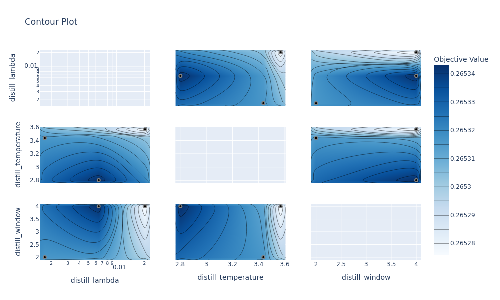
\includegraphics[width=\linewidth]{assets/plots/eval/porto/optuna/phase1/contour_plot.pdf}
        \caption{Parameter contour plot}
    \end{subfigure}
    \begin{subfigure}{0.49\linewidth}
        \centering
        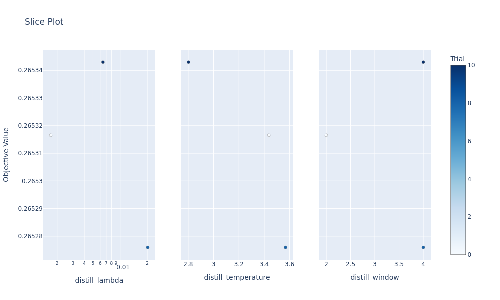
\includegraphics[width=\linewidth]{assets/plots/eval/porto/optuna/phase1/slice_plot.pdf}
        \caption{Parameter slice plot}
    \end{subfigure}
    \begin{subfigure}{0.49\linewidth}
        \centering
        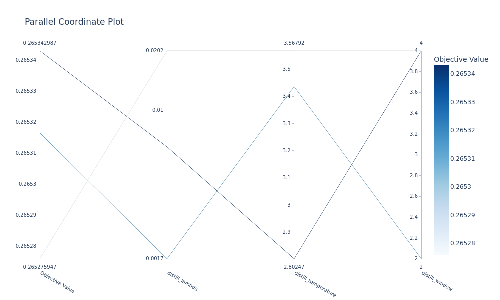
\includegraphics[width=\linewidth]{assets/plots/eval/porto/optuna/phase1/parallel_coordinate.pdf}
        \caption{Parallel coordinate plot}
    \end{subfigure}
    \caption{Porto Phase 1 hyperparameter optimization analysis. Contour and slice plots reveal parameter interactions and sensitivities. Parallel coordinates show trial progression through the search space.}
    \label{fig:appendix-optuna-phase1}
\end{figure}

\begin{figure}[H]
    \centering
    \begin{subfigure}{0.49\linewidth}
        \centering
        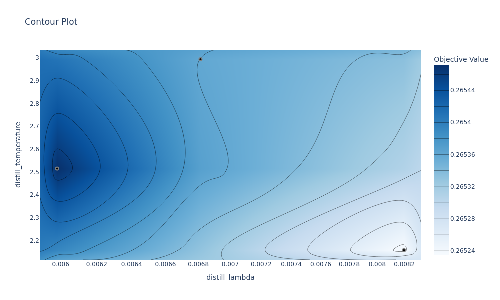
\includegraphics[width=\linewidth]{assets/plots/eval/porto/optuna/phase2/contour_plot.pdf}
        \caption{Parameter contour plot}
    \end{subfigure}
    \begin{subfigure}{0.49\linewidth}
        \centering
        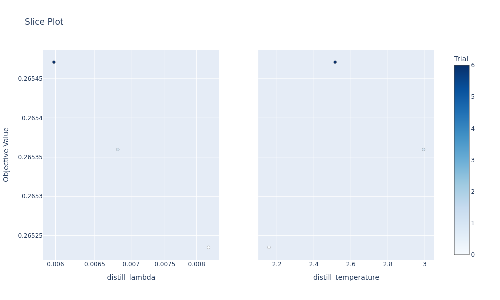
\includegraphics[width=\linewidth]{assets/plots/eval/porto/optuna/phase2/slice_plot.pdf}
        \caption{Parameter slice plot}
    \end{subfigure}
    \begin{subfigure}{0.49\linewidth}
        \centering
        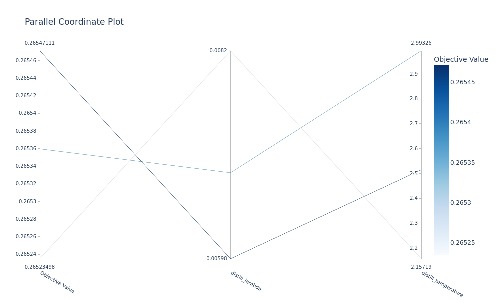
\includegraphics[width=\linewidth]{assets/plots/eval/porto/optuna/phase2/parallel_coordinate.pdf}
        \caption{Parallel coordinate plot}
    \end{subfigure}
    \caption{Porto Phase 2 hyperparameter optimization analysis. Refinement phase shows tighter parameter distributions and more consistent trial performance compared to Phase 1.}
    \label{fig:appendix-optuna-phase2}
\end{figure}

\subsubsection{Scenario-Level Analysis (Beijing)}
\label{app:scenario-beijing}

Figures~\ref{fig:appendix-beijing-scenario-heatmap} through~\ref{fig:appendix-beijing-scenario-spatial} present scenario-level performance breakdowns for Beijing, supporting the context-dependent analysis in \autoref{sec:eval-beijing}.

\begin{figure}[H]
    \centering
    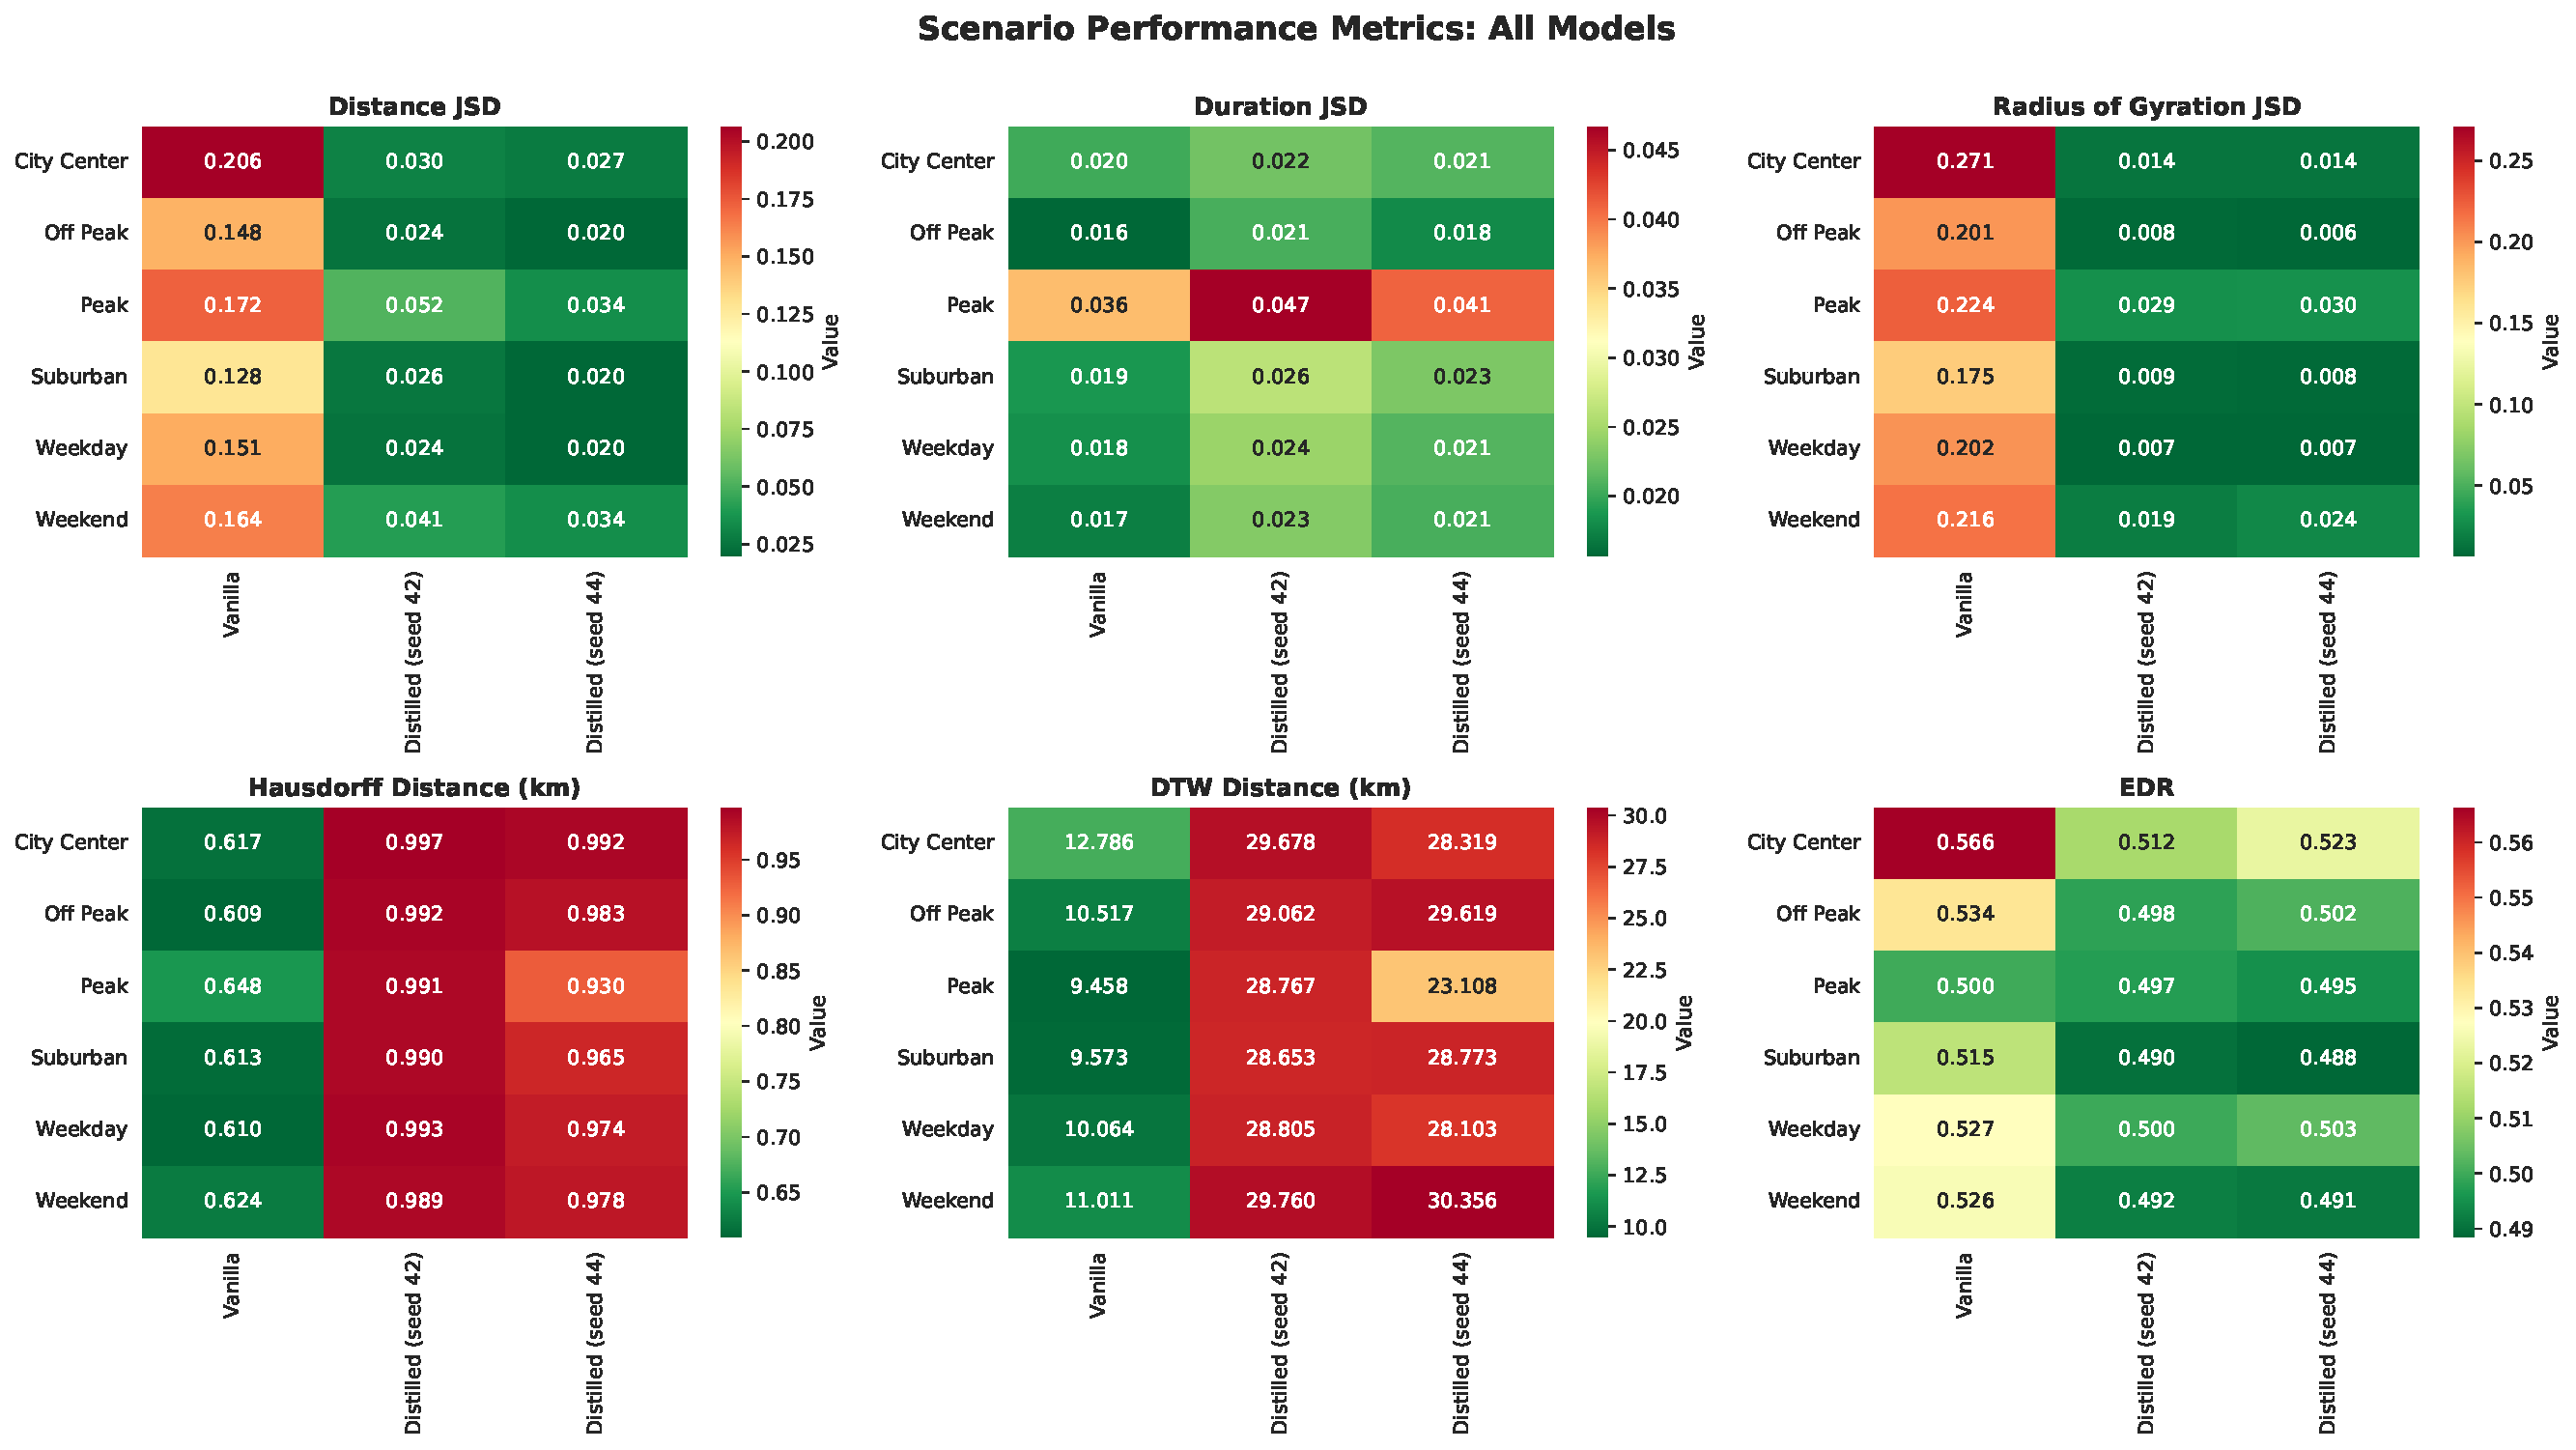
\includegraphics[width=0.85\linewidth]{assets/plots/eval/beijing/scenarios/scenario_metrics_heatmap.pdf}
    \caption{Beijing scenario-level metrics heatmap showing performance across spatial and temporal contexts. Distilled models maintain consistent high performance across all scenarios.}
    \label{fig:appendix-beijing-scenario-heatmap}
\end{figure}

\begin{figure}[H]
    \centering
    \begin{subfigure}{0.49\linewidth}
        \centering
        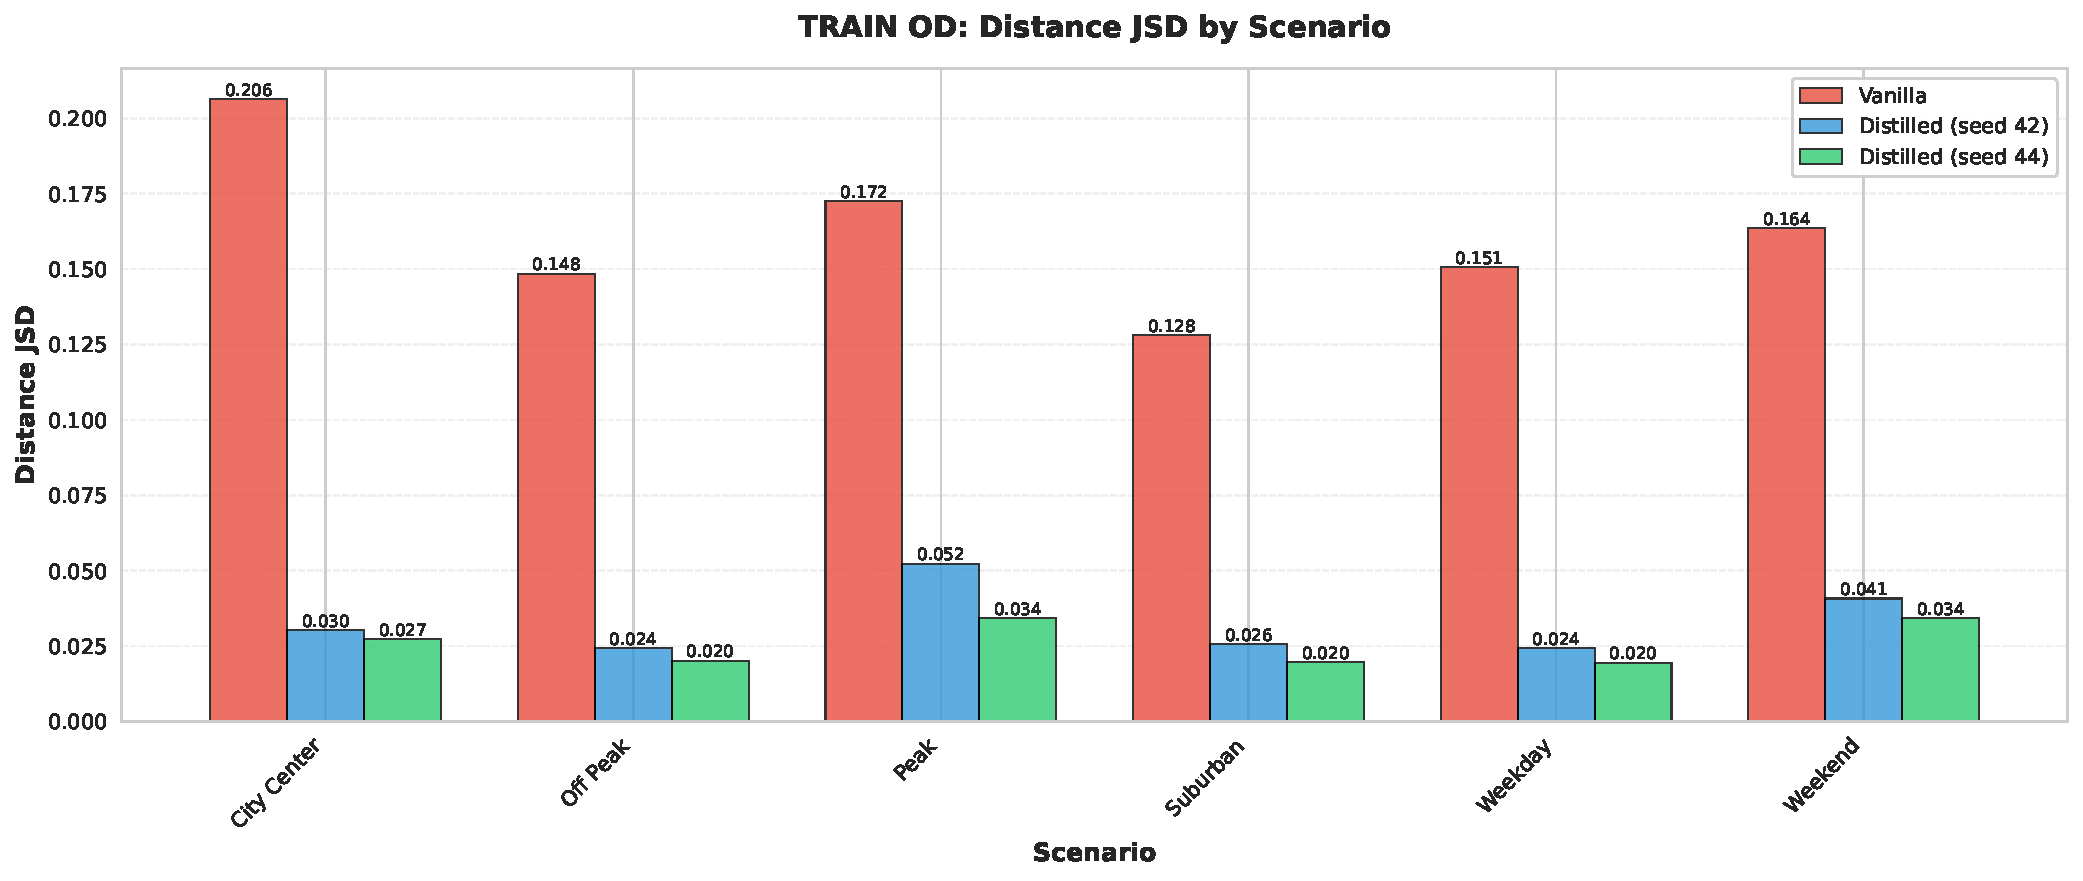
\includegraphics[width=\linewidth]{assets/plots/eval/beijing/scenarios/train_od_scenario_comparison.pdf}
        \caption{Train OD scenarios}
    \end{subfigure}
    \begin{subfigure}{0.49\linewidth}
        \centering
        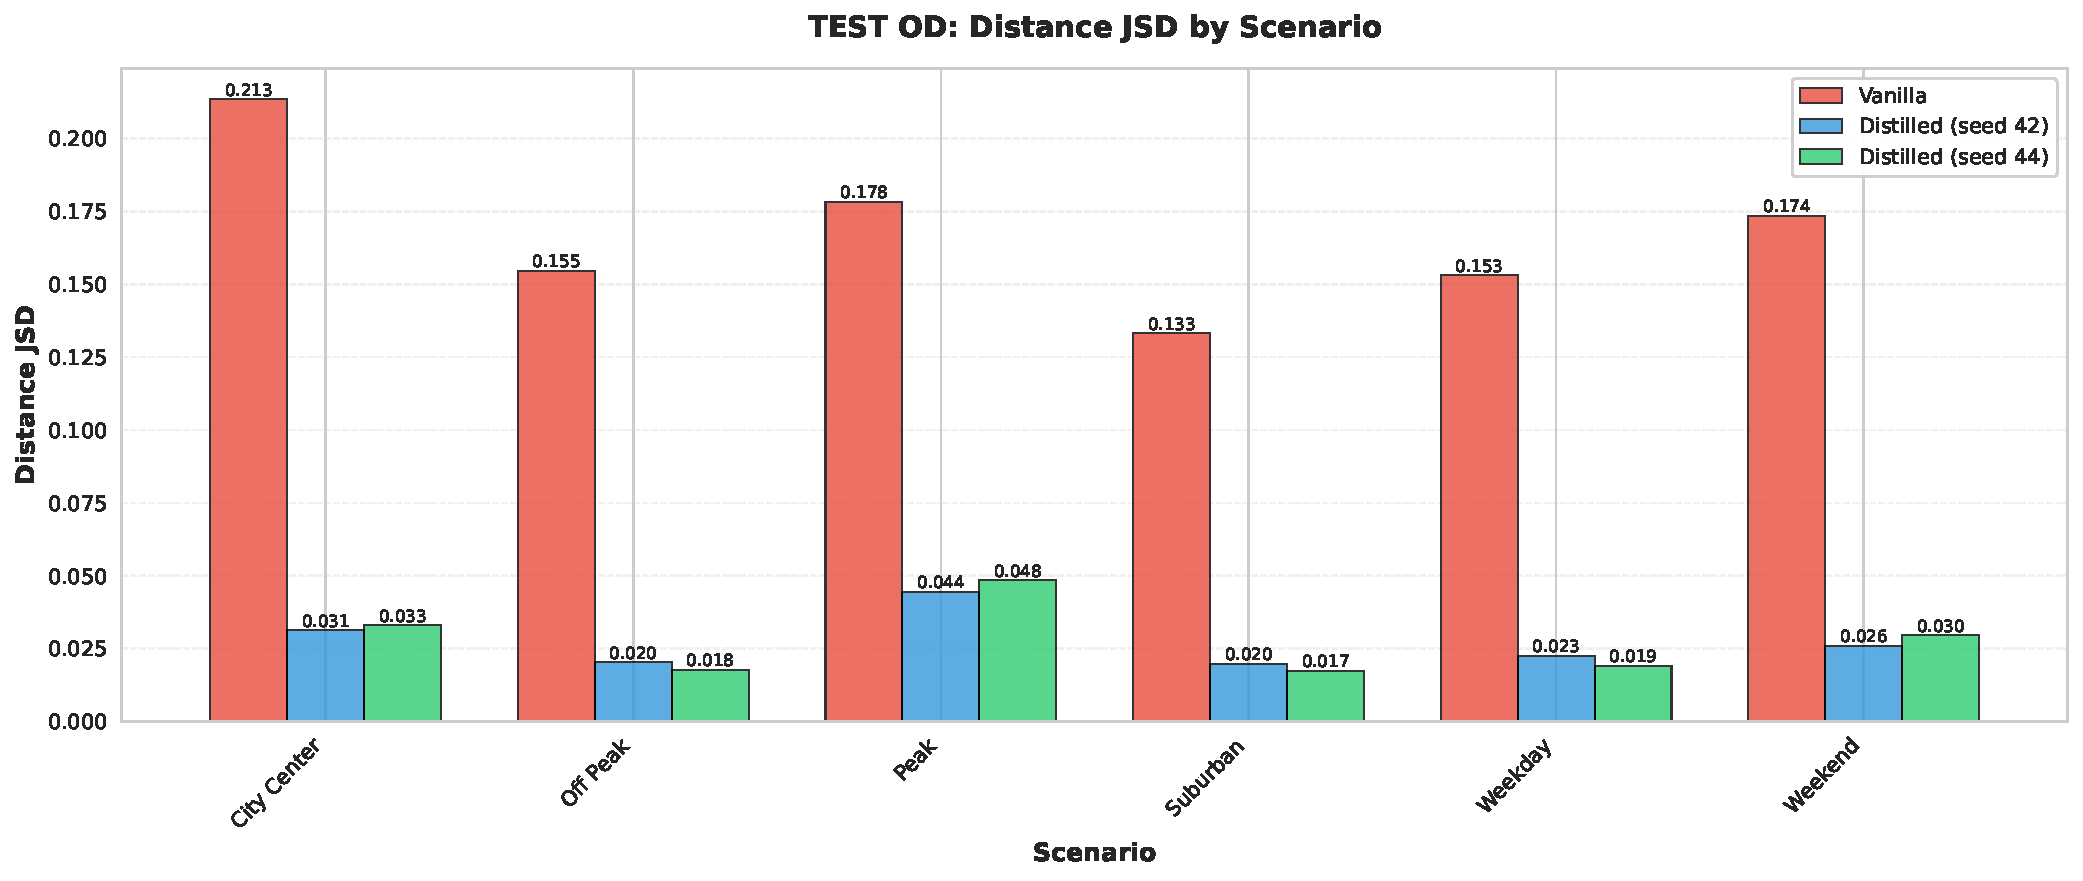
\includegraphics[width=\linewidth]{assets/plots/eval/beijing/scenarios/test_od_scenario_comparison.pdf}
        \caption{Test OD scenarios}
    \end{subfigure}
    \caption{Beijing scenario comparison across train and test OD pairs. Distilled models show consistent superiority regardless of spatial or temporal context.}
    \label{fig:appendix-beijing-scenario-comparison}
\end{figure}

\begin{figure}[H]
    \centering
    \begin{subfigure}{0.49\linewidth}
        \centering
        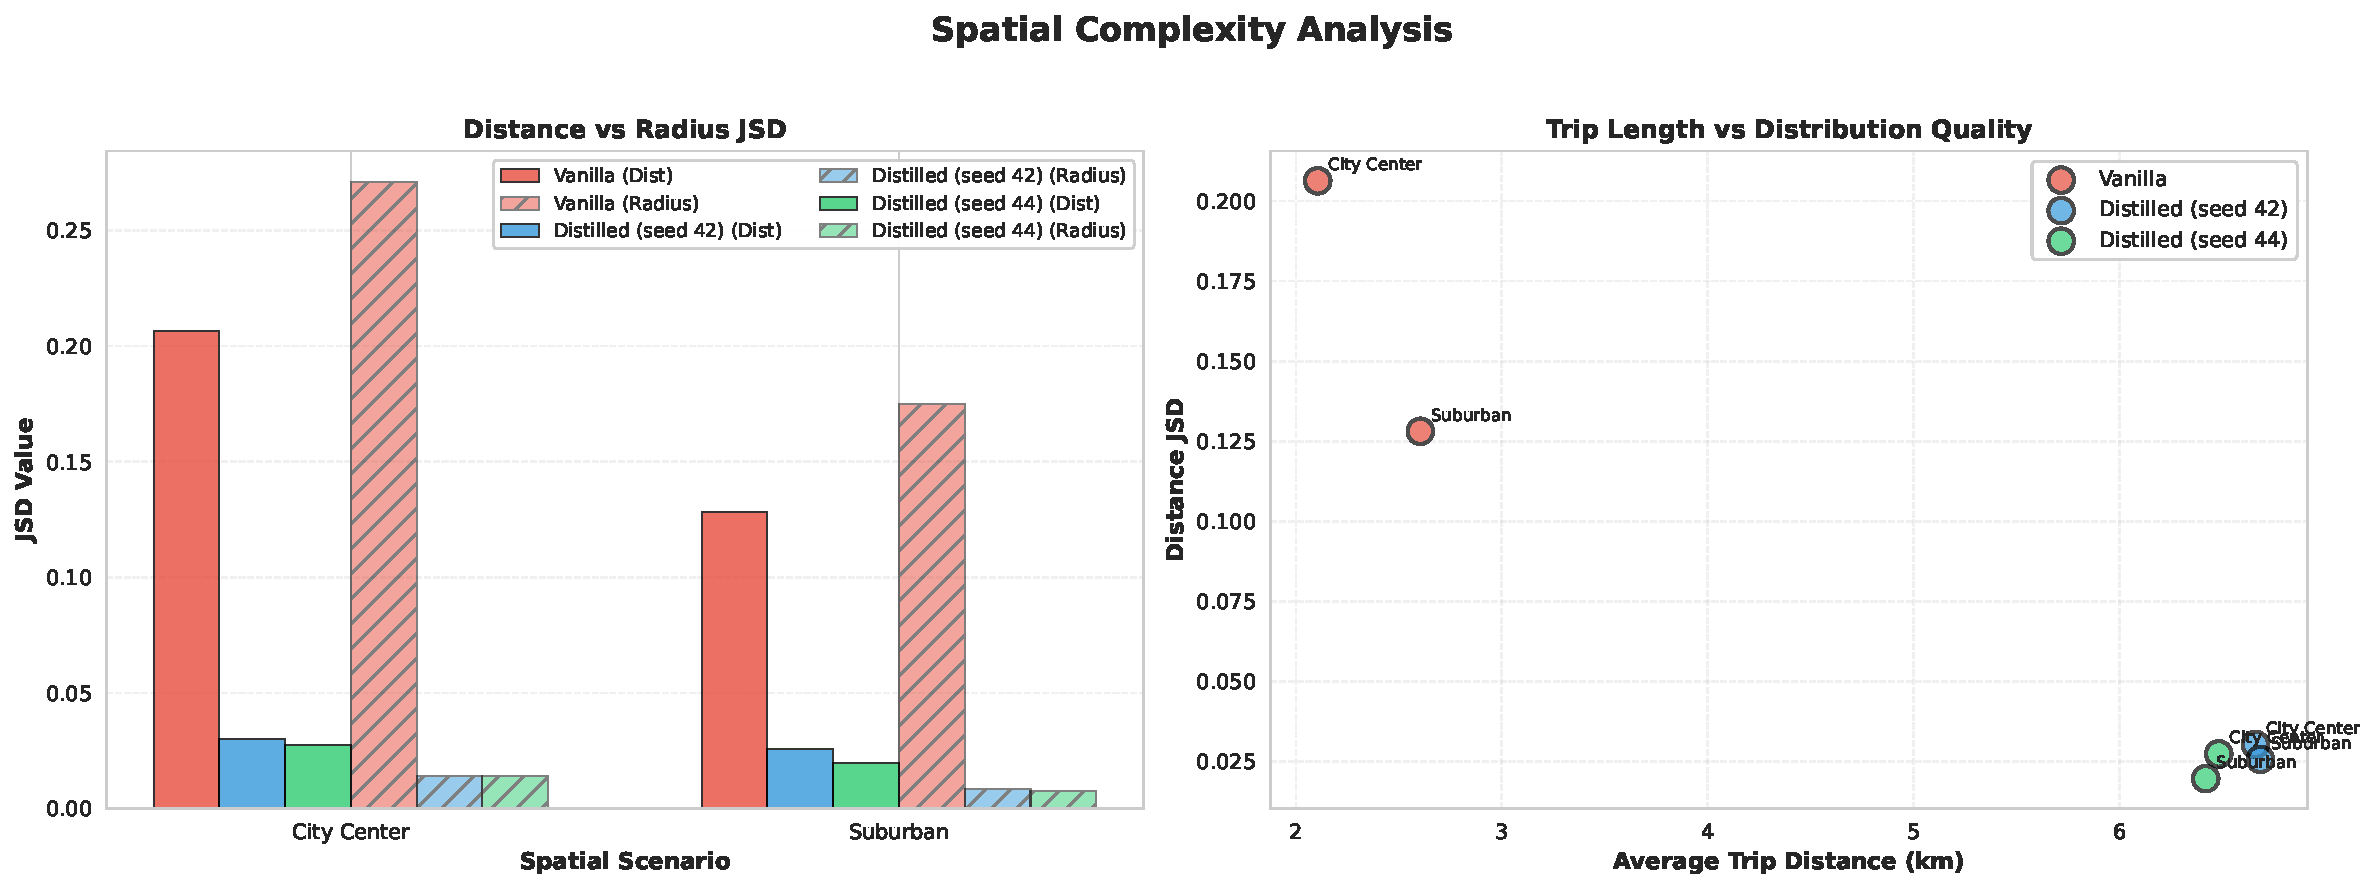
\includegraphics[width=\linewidth]{assets/plots/eval/beijing/scenarios/spatial_scenarios_analysis.pdf}
        \caption{Spatial context analysis}
    \end{subfigure}
    \begin{subfigure}{0.49\linewidth}
        \centering
        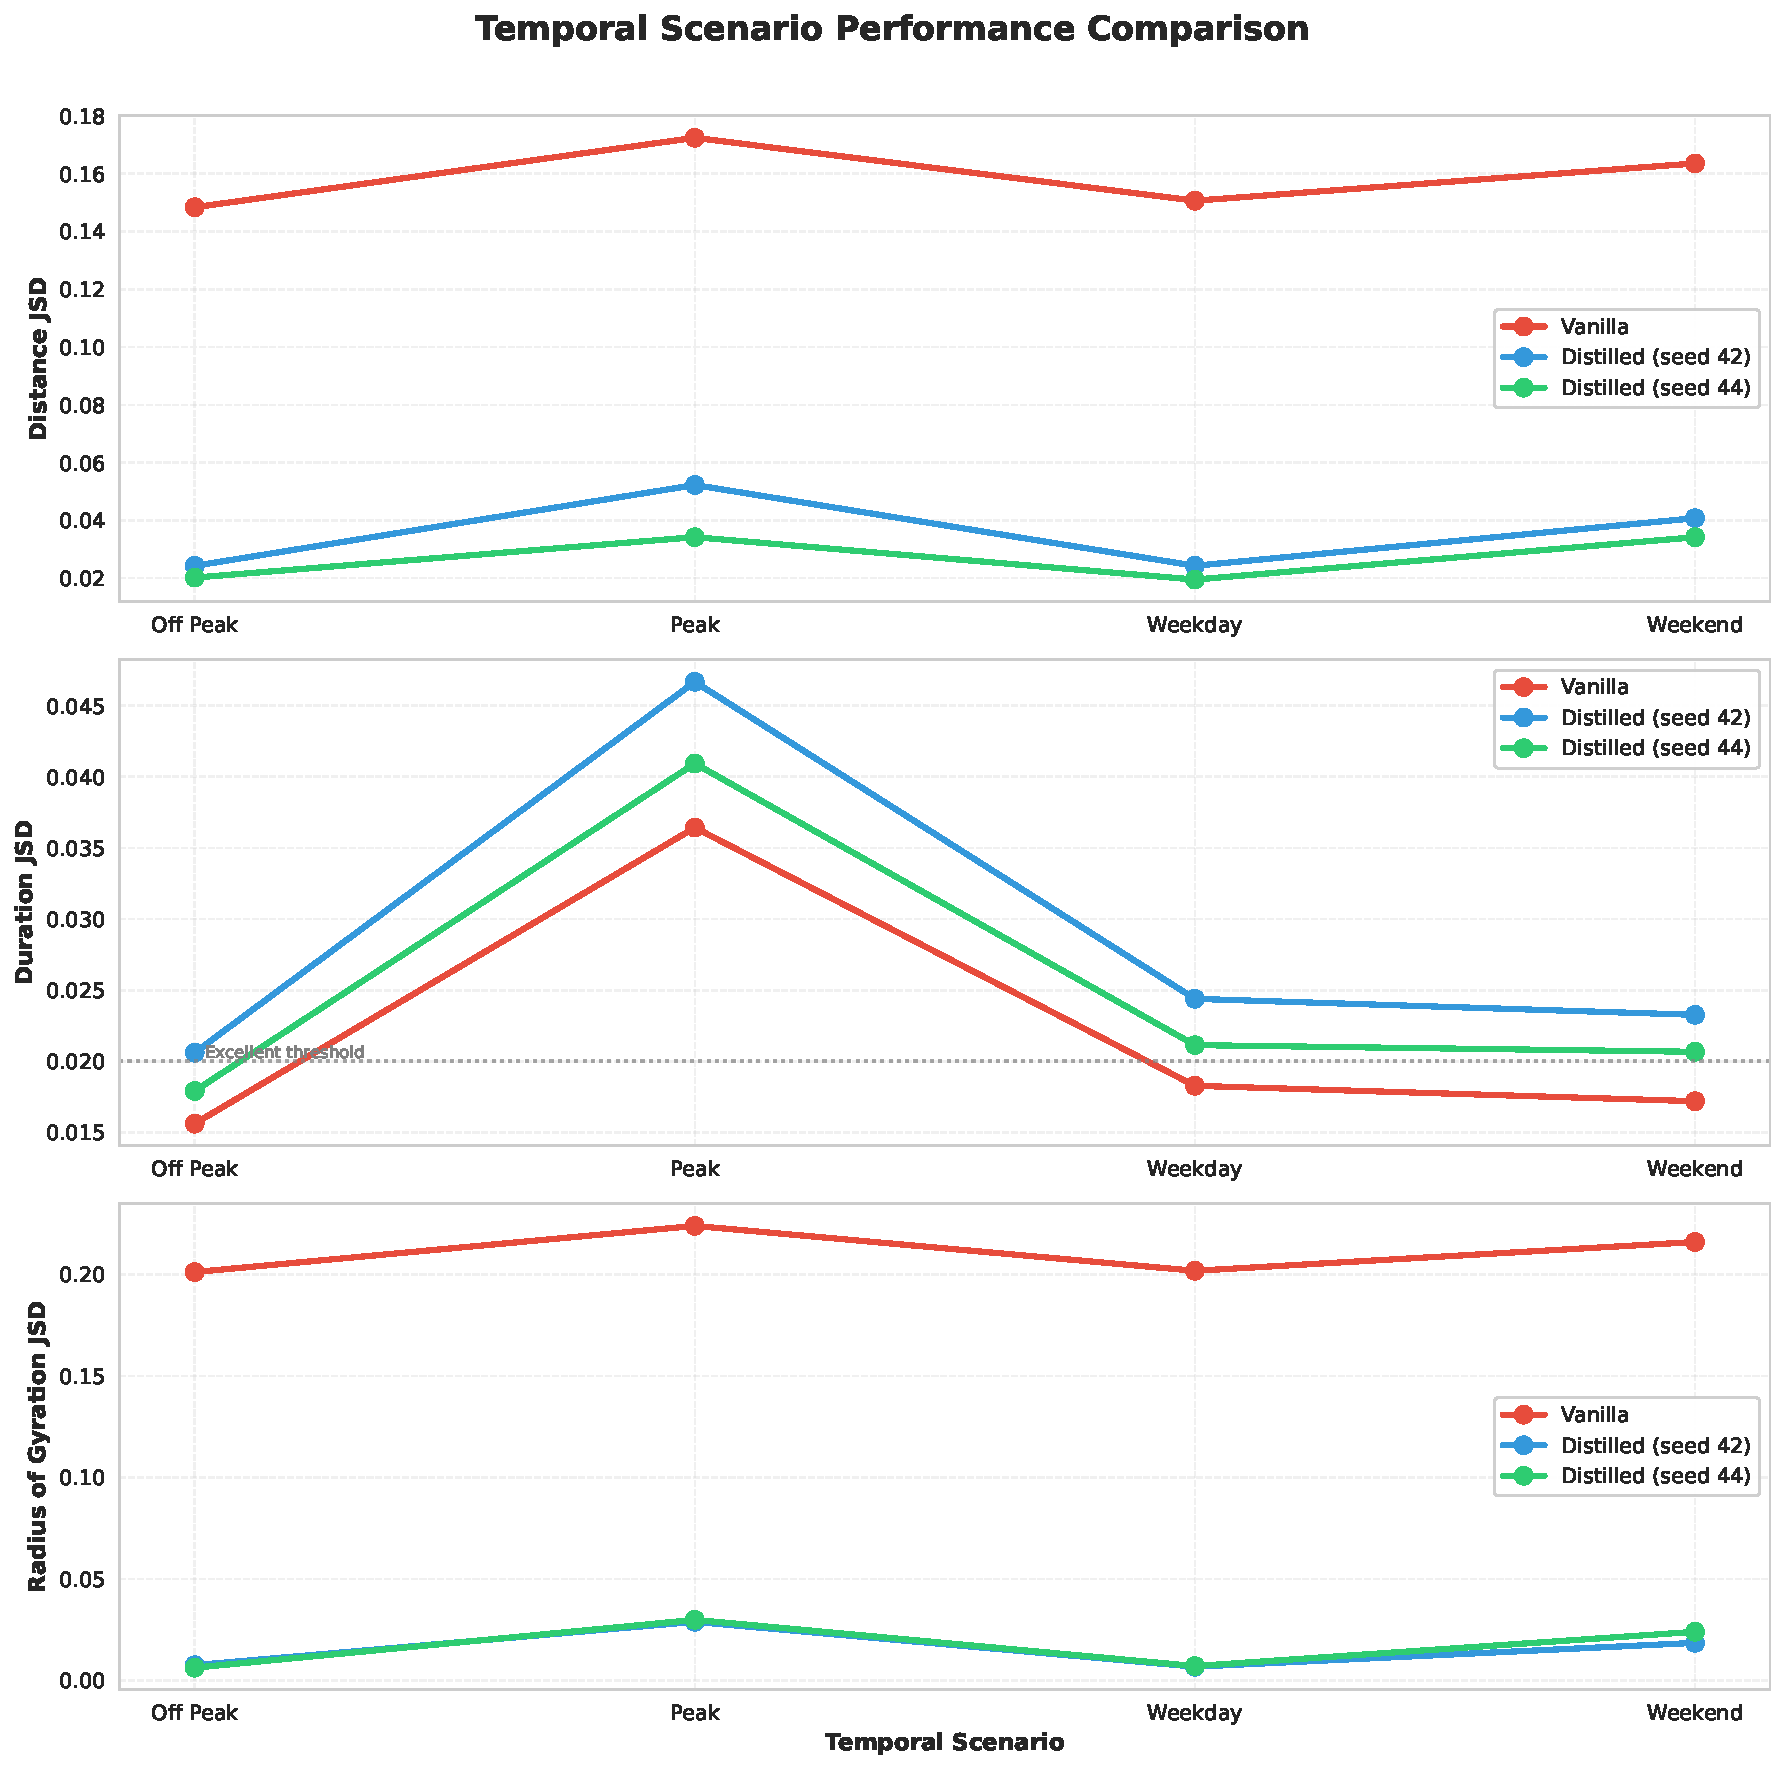
\includegraphics[width=\linewidth]{assets/plots/eval/beijing/scenarios/temporal_scenarios_comparison.pdf}
        \caption{Temporal context analysis}
    \end{subfigure}
    \caption{Beijing spatial and temporal scenario performance. Universal improvement across all contexts demonstrates robust knowledge transfer.}
    \label{fig:appendix-beijing-scenario-spatial}
\end{figure}

\subsubsection{Scenario-Level Analysis (Porto)}
\label{app:scenario-porto}

Figures~\ref{fig:appendix-porto-scenario-heatmap} through~\ref{fig:appendix-porto-scenario-sensitivity} present scenario-level performance breakdowns for Porto, revealing context-dependent behavior discussed in \autoref{sec:eval-porto}.

\begin{figure}[H]
    \centering
    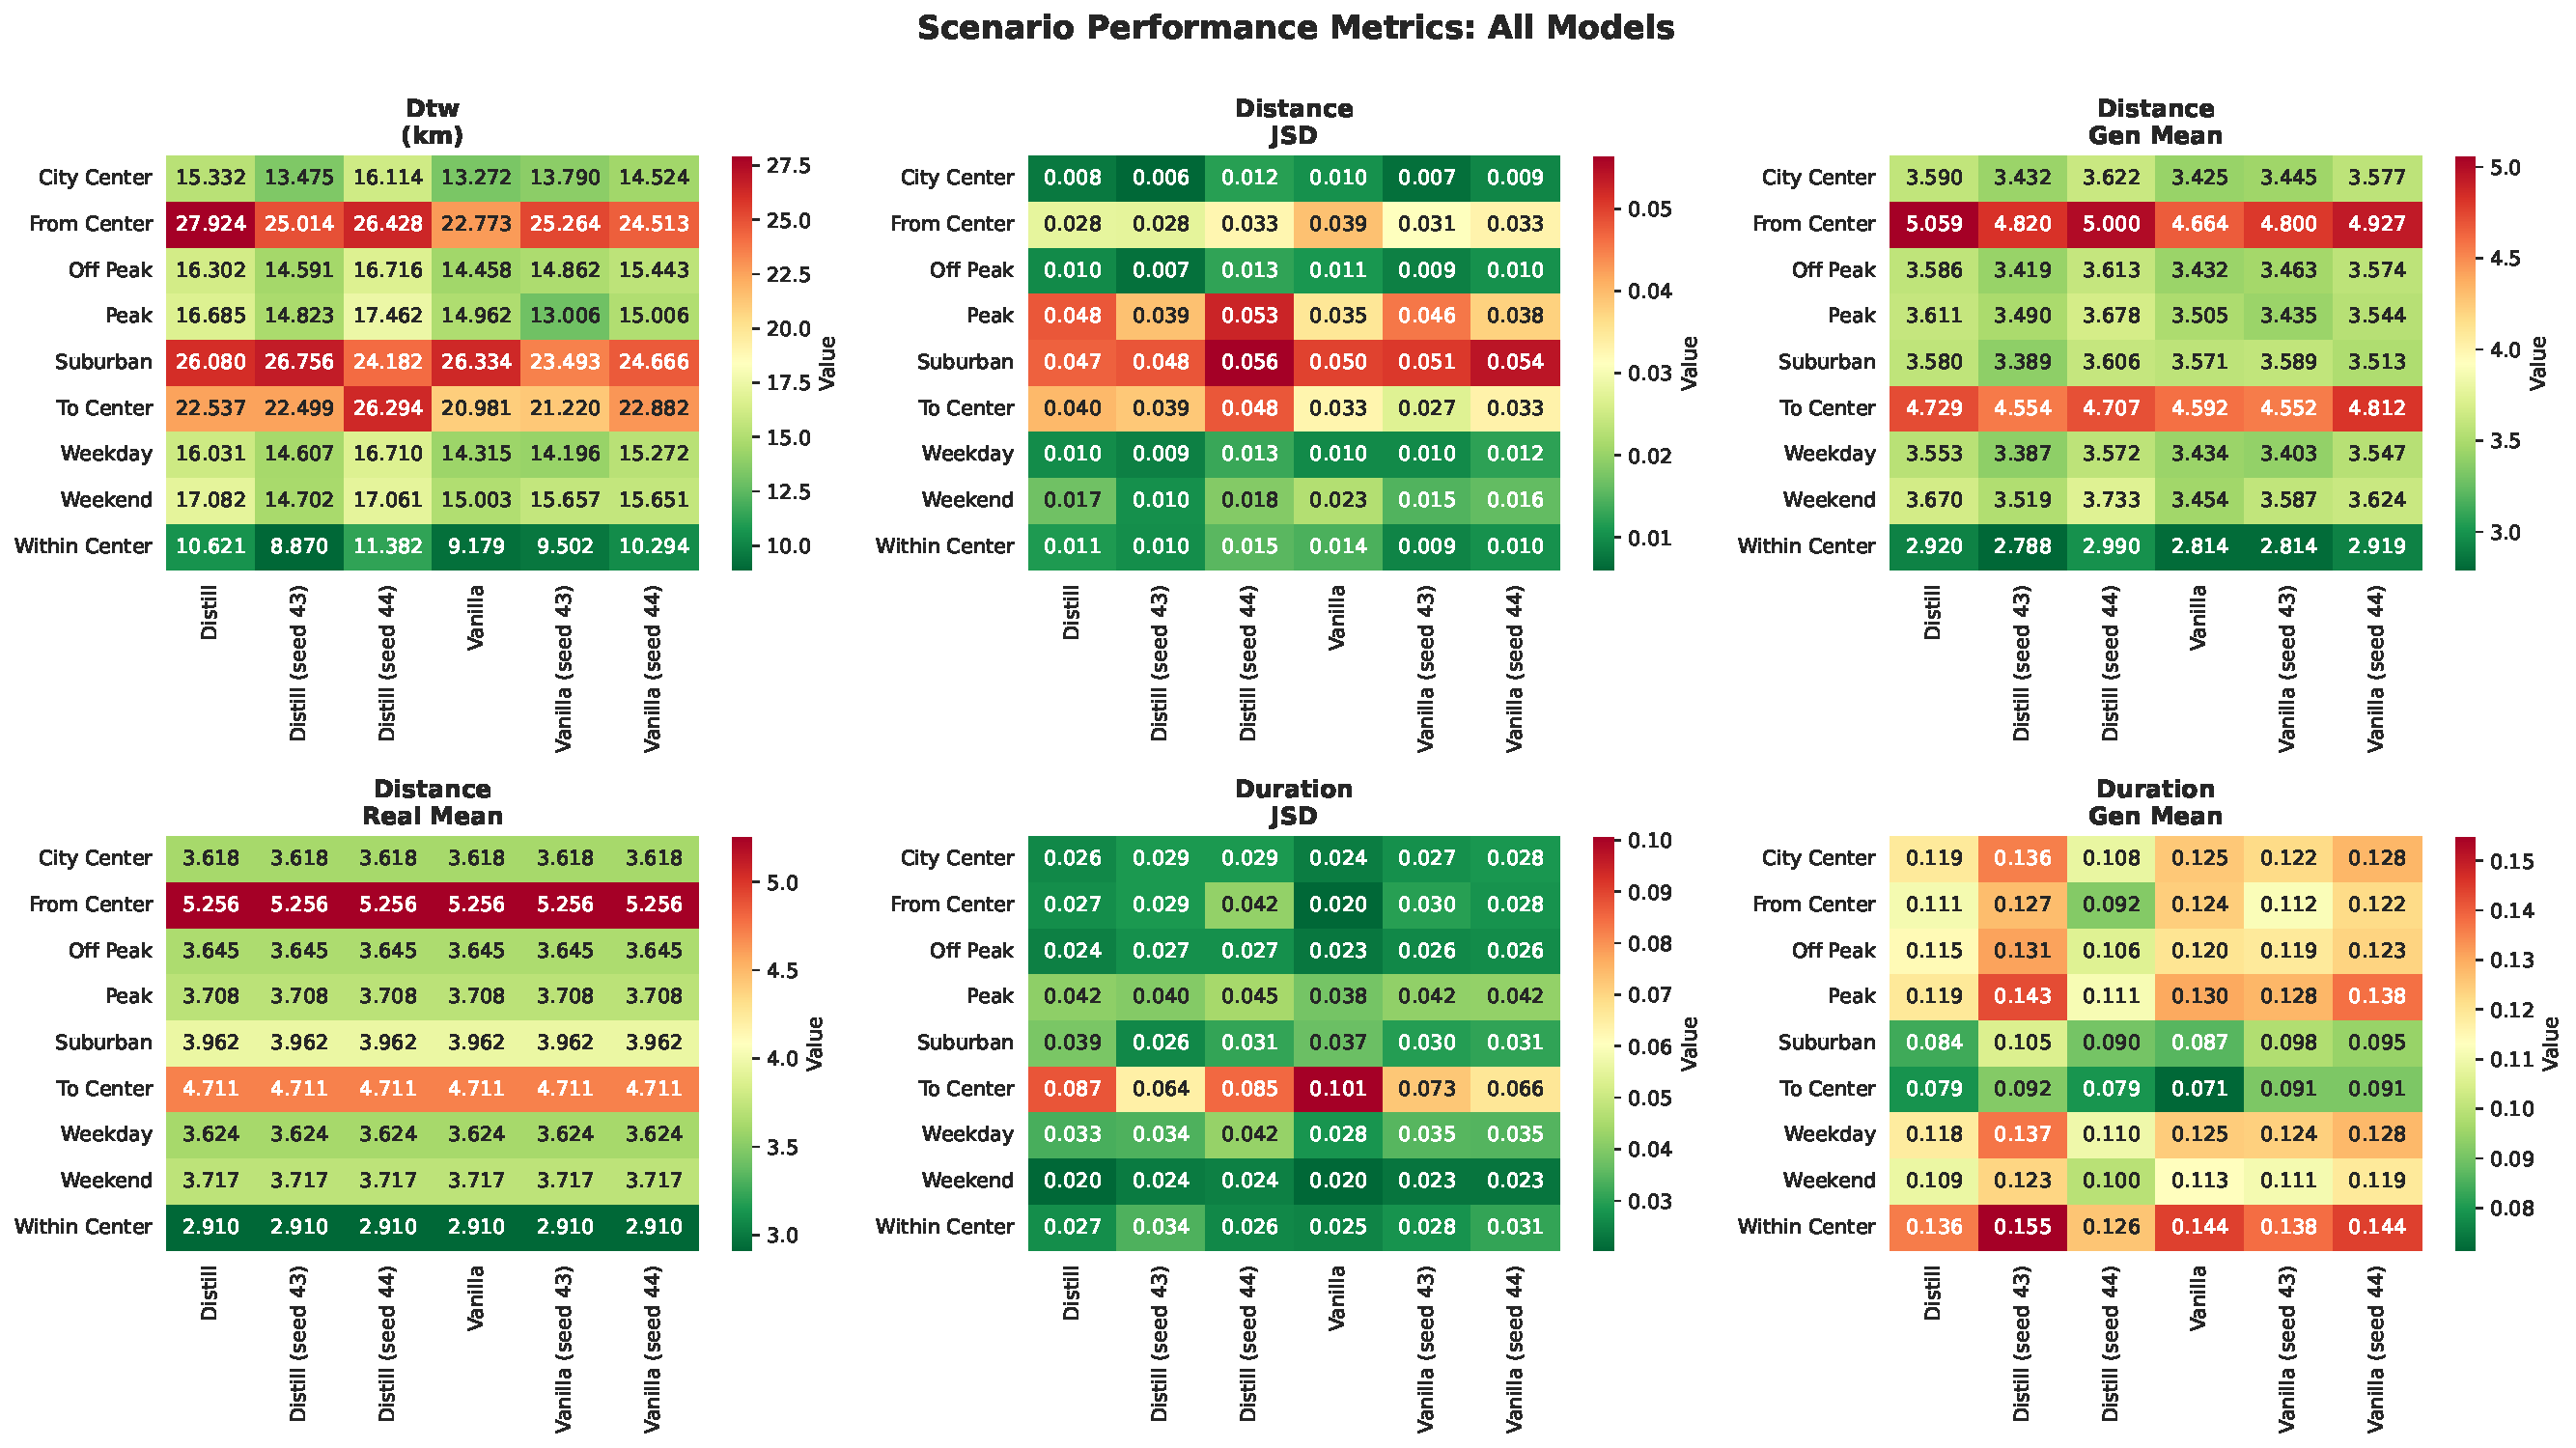
\includegraphics[width=0.85\linewidth]{assets/plots/eval/porto/scenarios/scenario_metrics_heatmap.pdf}
    \caption{Porto scenario-level metrics heatmap showing spatially localized performance gains. Distillation benefits concentrate in suburban and rural contexts.}
    \label{fig:appendix-porto-scenario-heatmap}
\end{figure}

\begin{figure}[H]
    \centering
    \begin{subfigure}{0.49\linewidth}
        \centering
        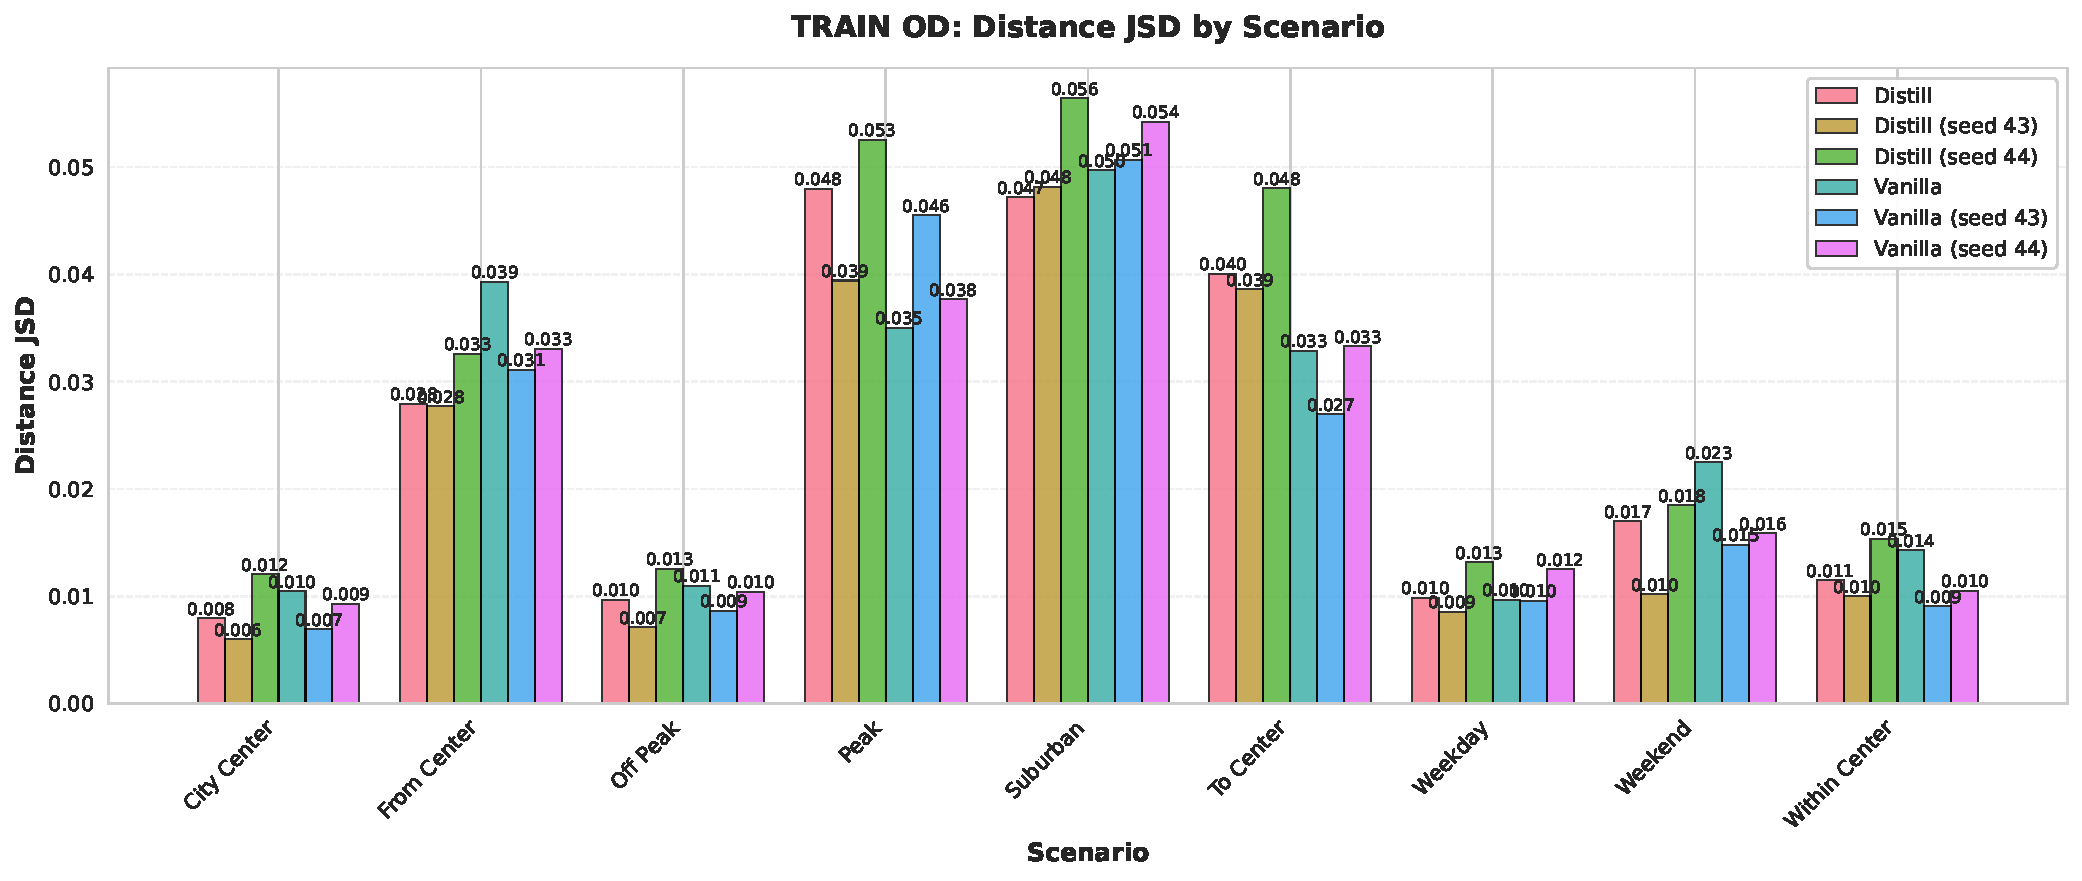
\includegraphics[width=\linewidth]{assets/plots/eval/porto/scenarios/train_od_scenario_comparison.pdf}
        \caption{Train OD scenarios}
    \end{subfigure}
    \begin{subfigure}{0.49\linewidth}
        \centering
        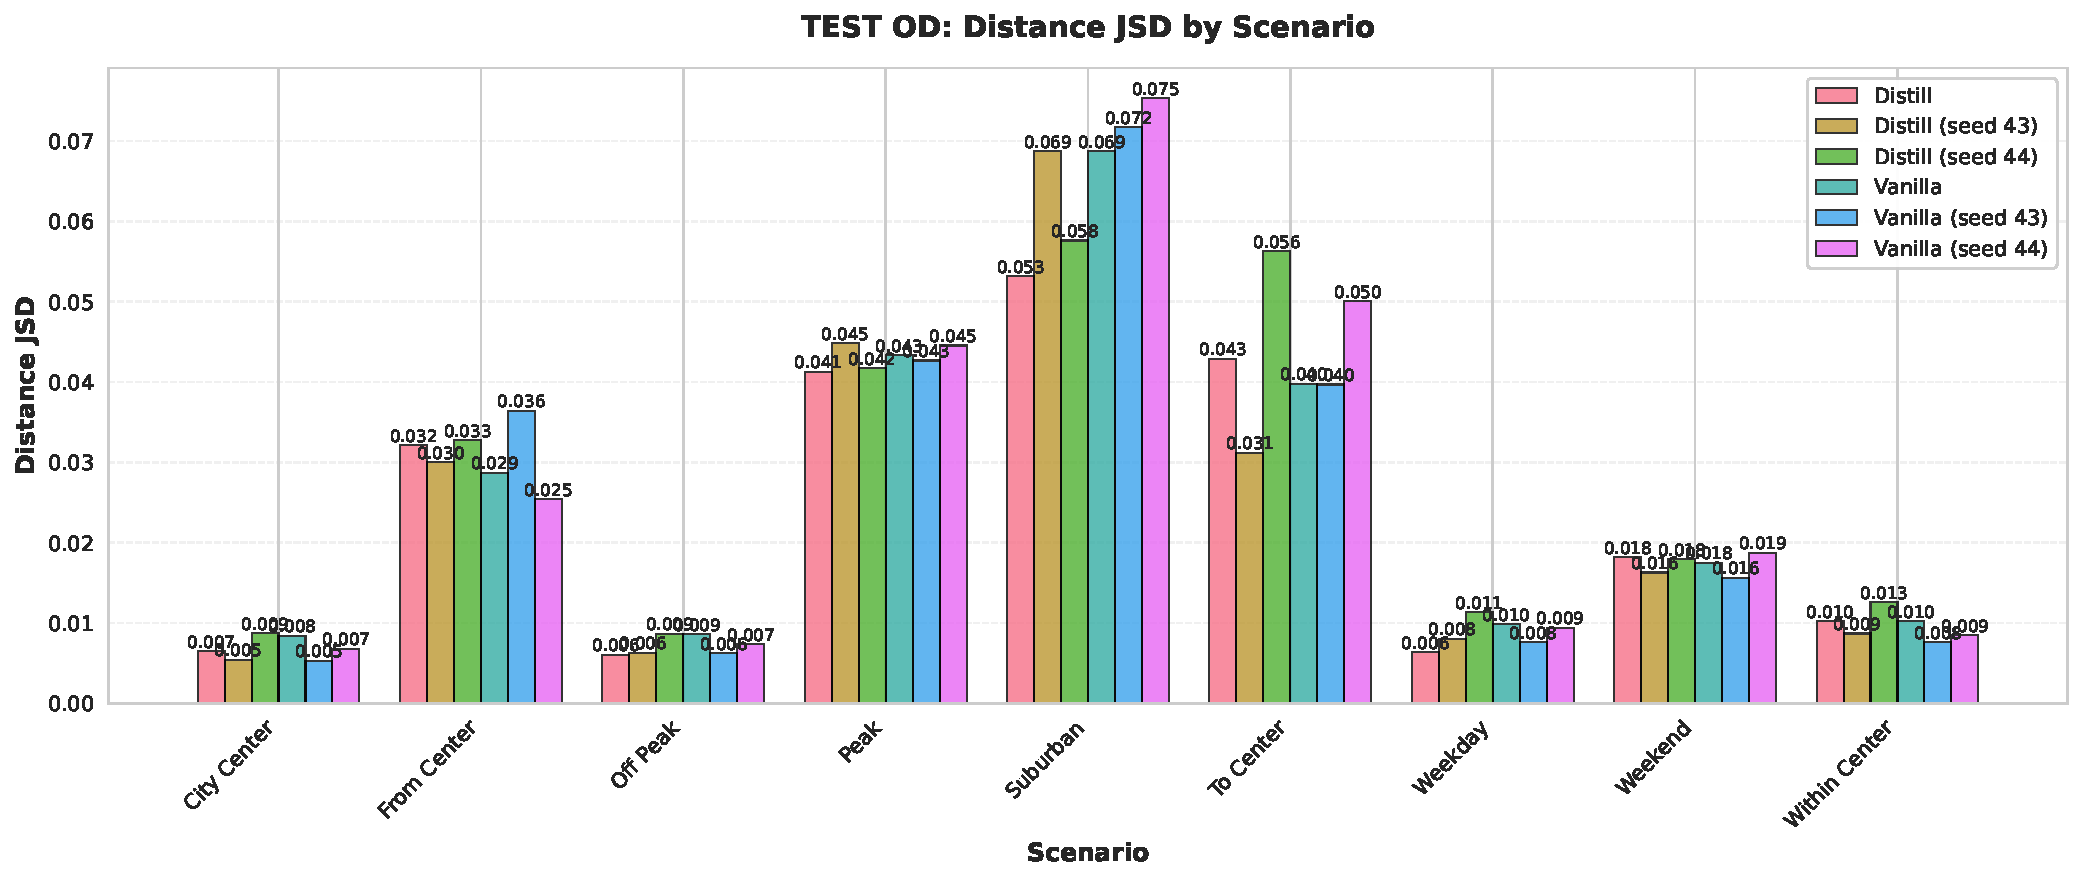
\includegraphics[width=\linewidth]{assets/plots/eval/porto/scenarios/test_od_scenario_comparison.pdf}
        \caption{Test OD scenarios}
    \end{subfigure}
    \caption{Porto scenario comparison across train and test OD pairs. Performance varies by spatial context, with stronger improvements in less urbanized areas.}
    \label{fig:appendix-porto-scenario-comparison}
\end{figure}

\begin{figure}[H]
    \centering
    \begin{subfigure}{0.49\linewidth}
        \centering
        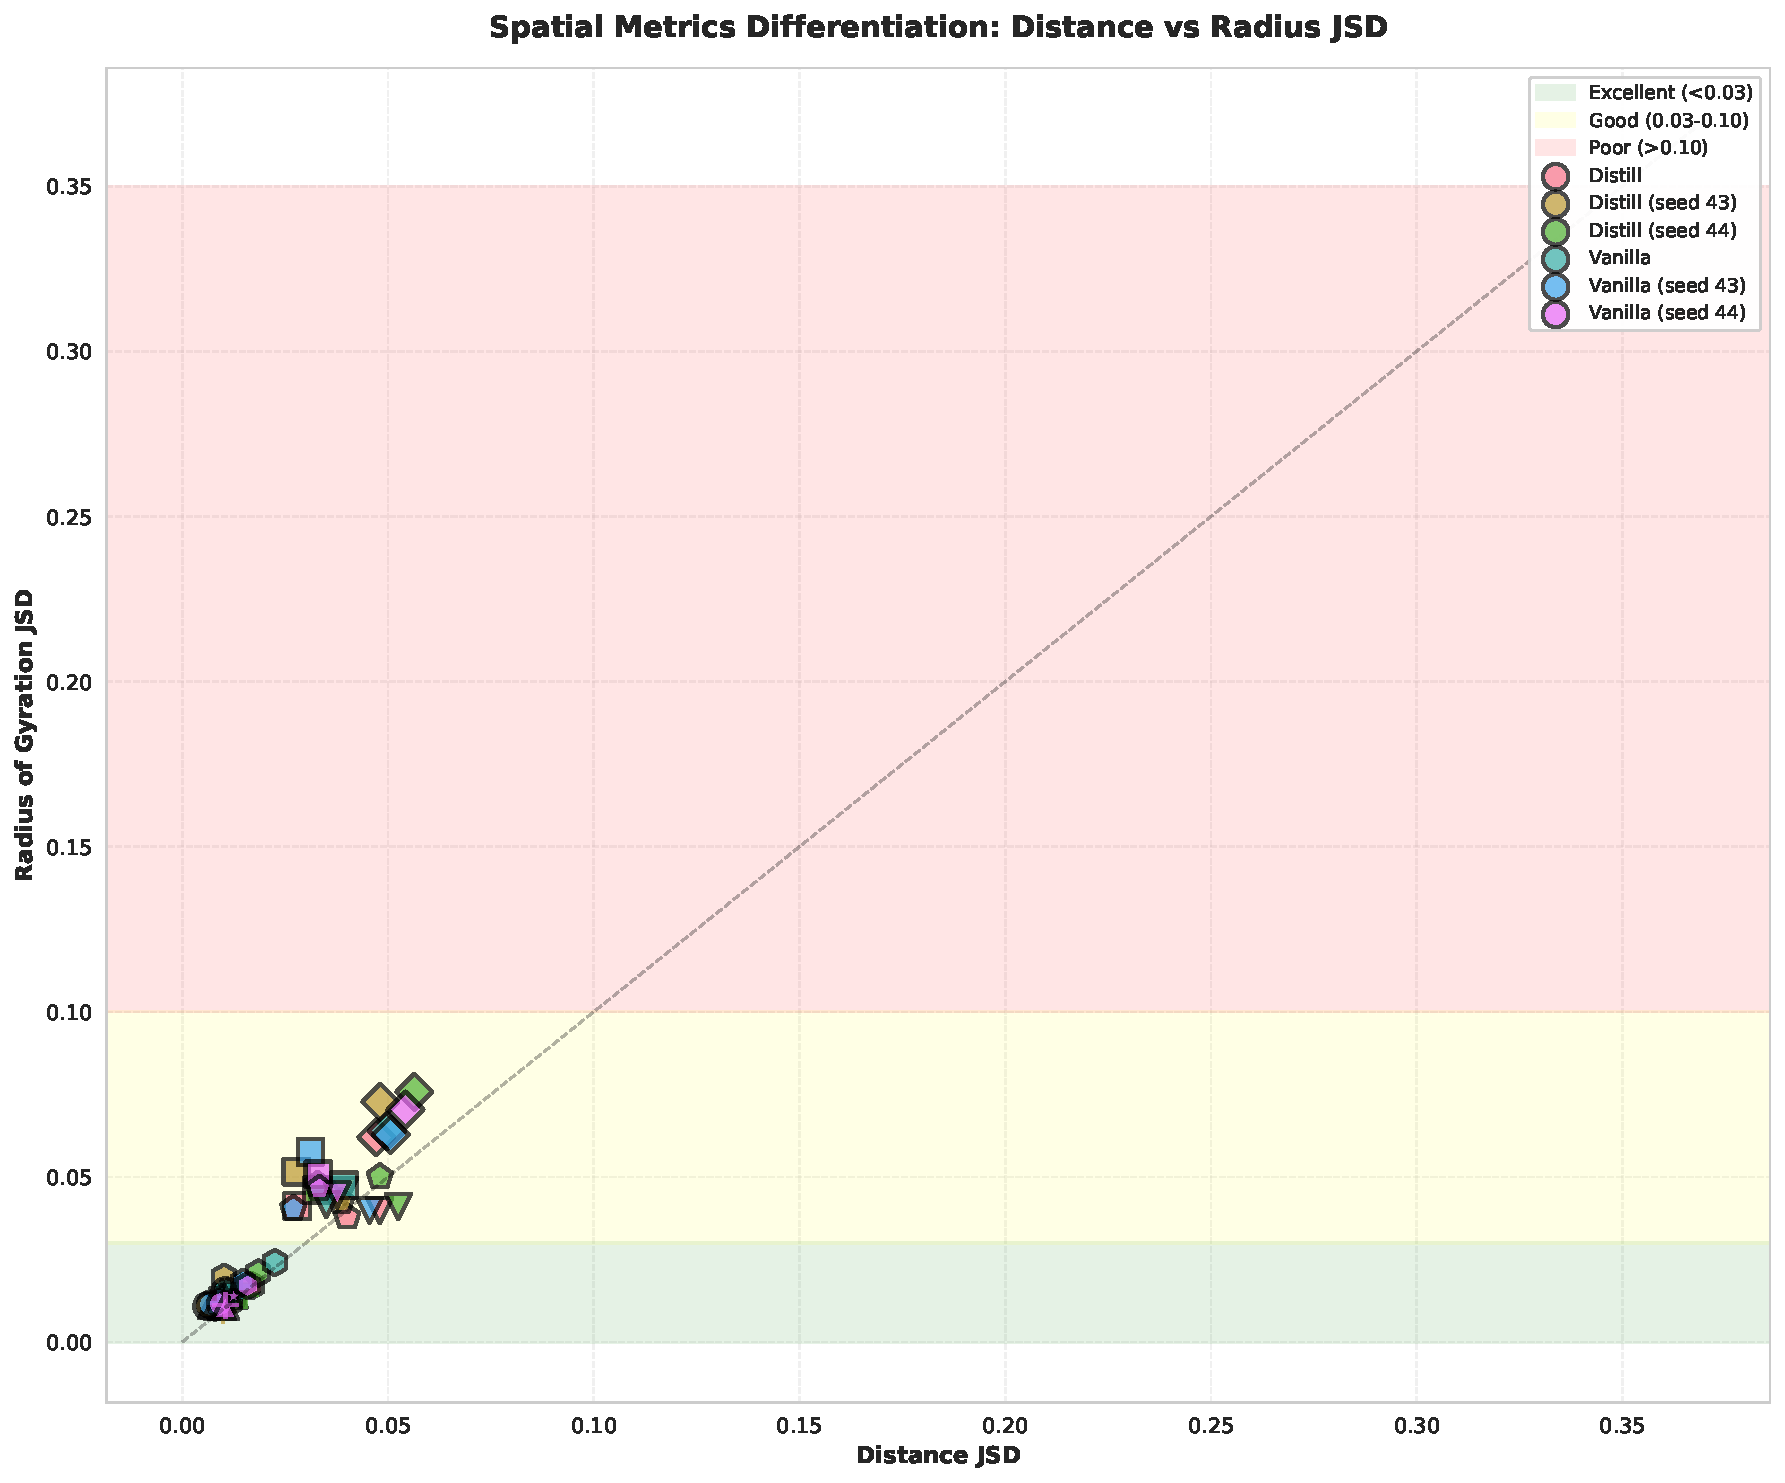
\includegraphics[width=\linewidth]{assets/plots/eval/porto/scenarios/spatial_metrics_differentiation.pdf}
        \caption{Spatial differentiation}
    \end{subfigure}
    \begin{subfigure}{0.49\linewidth}
        \centering
        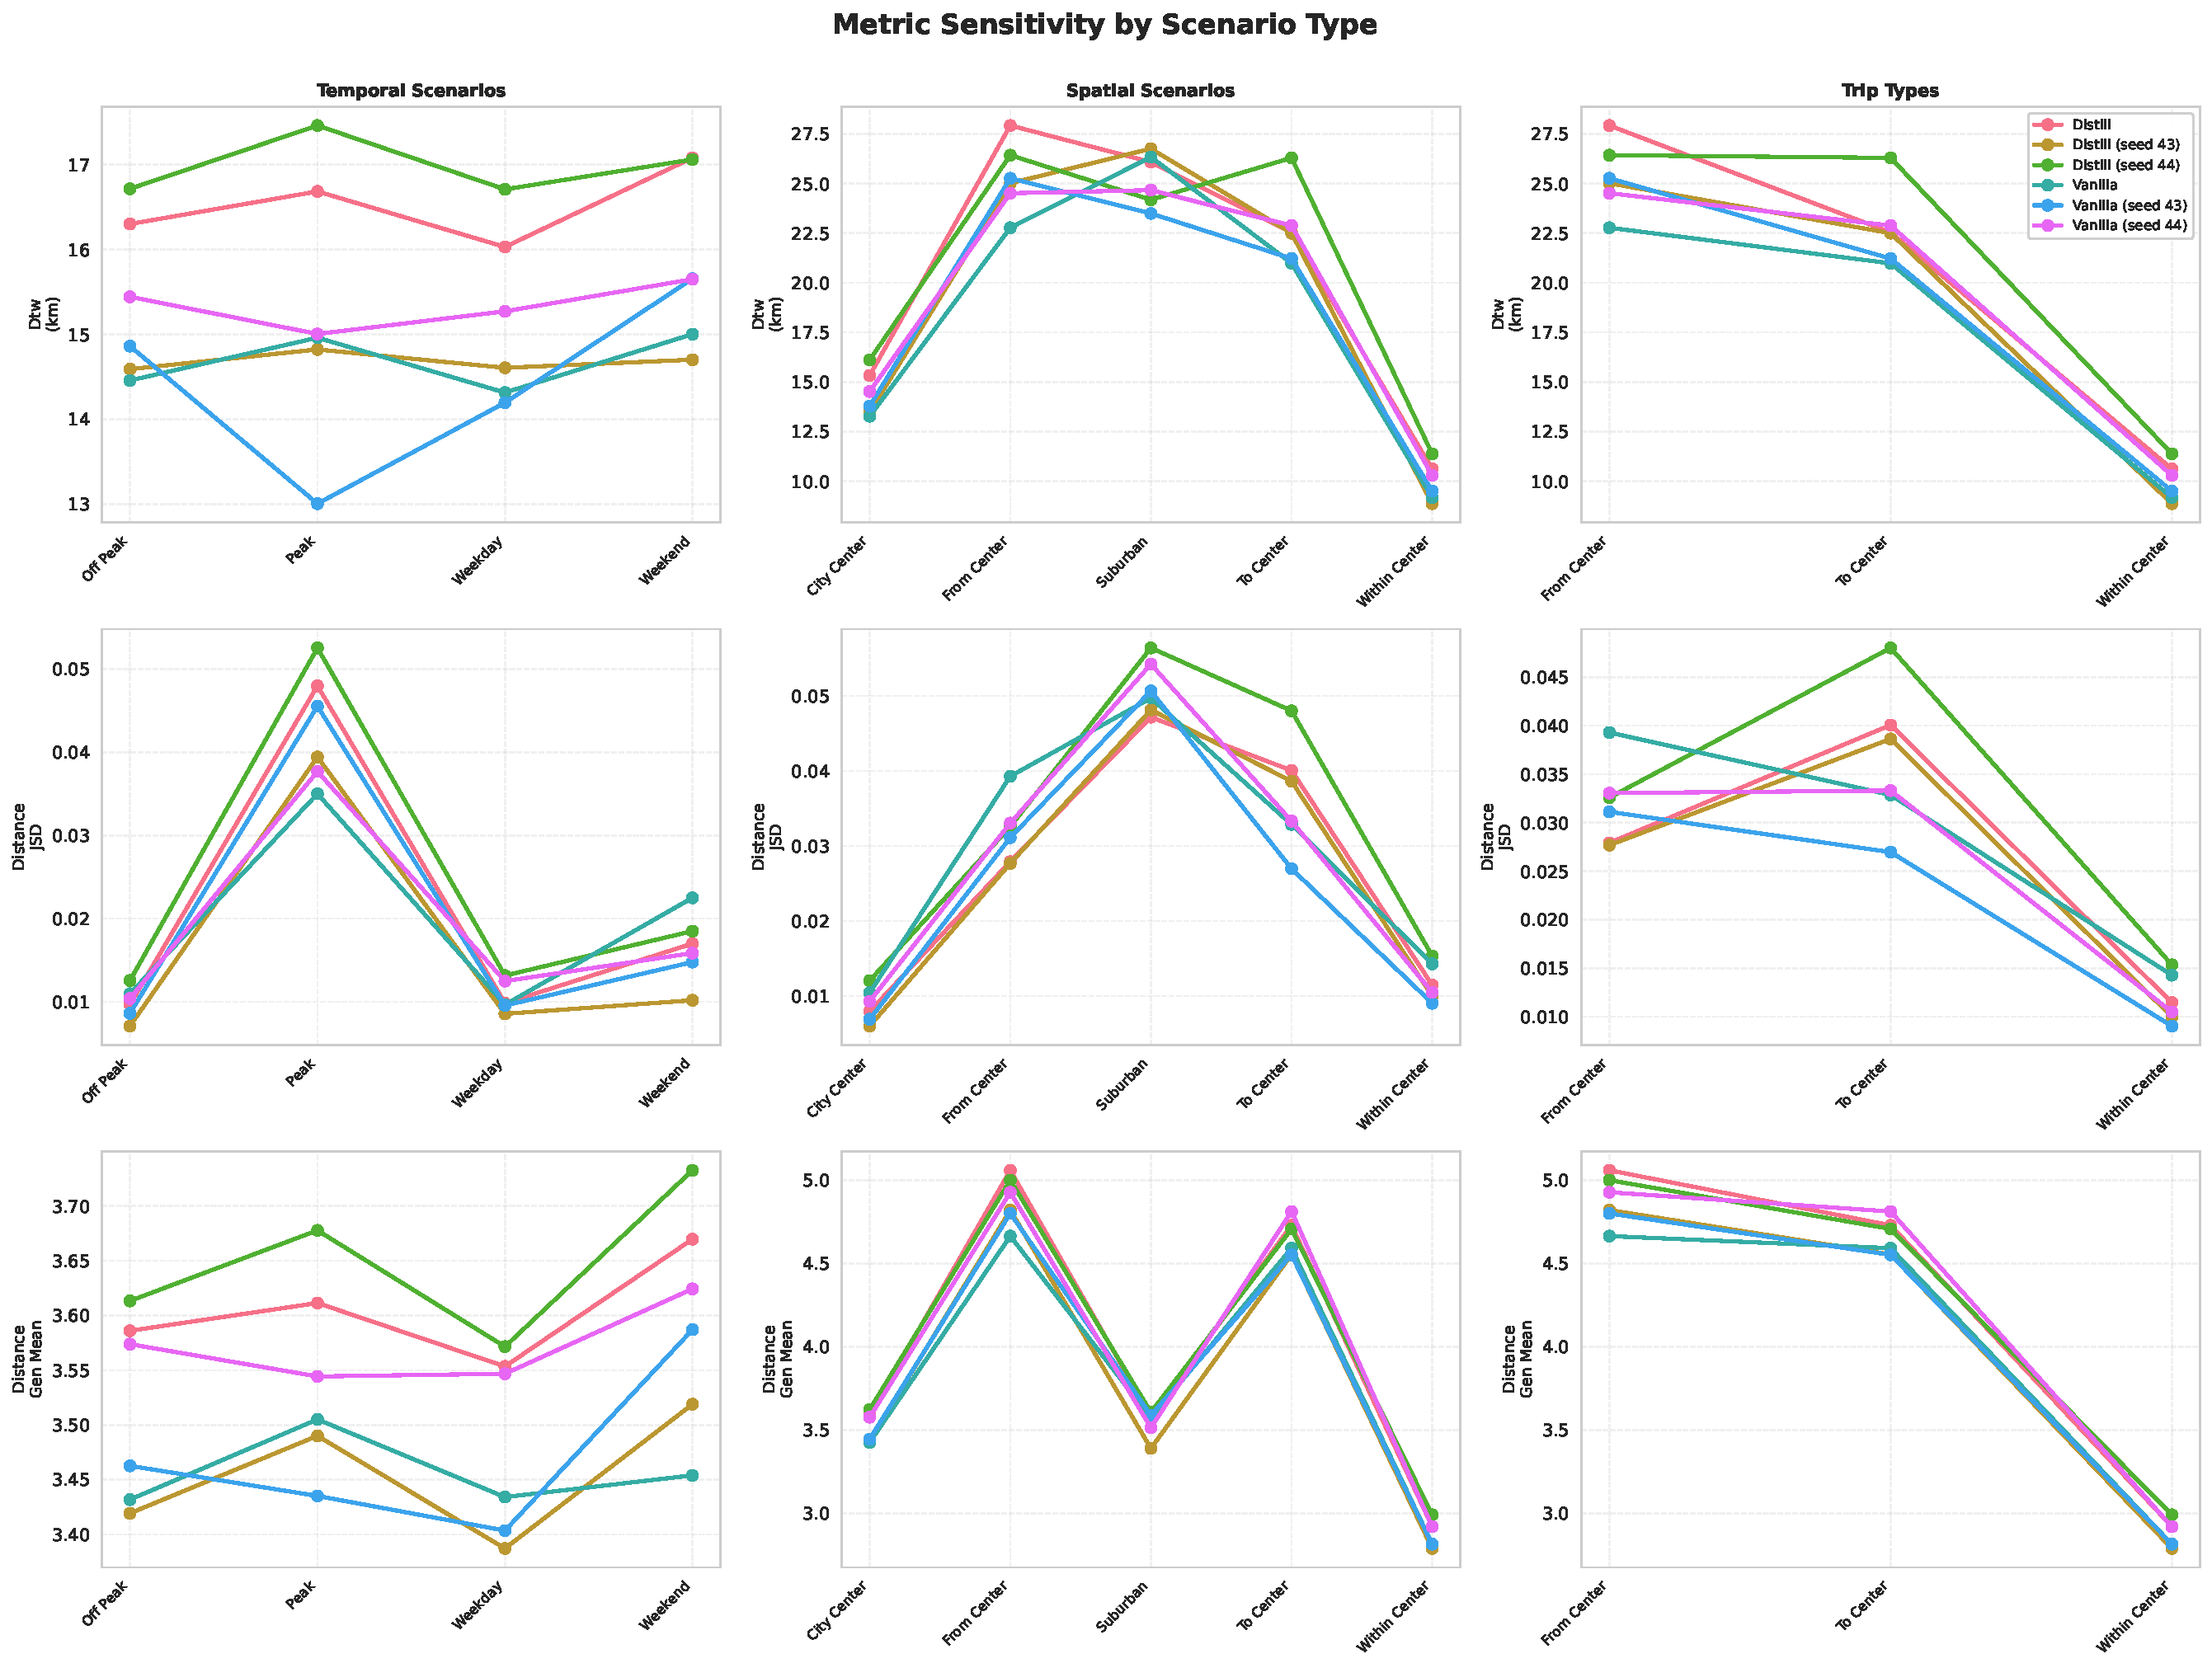
\includegraphics[width=\linewidth]{assets/plots/eval/porto/scenarios/metric_sensitivity_by_scenario.pdf}
        \caption{Metric sensitivity}
    \end{subfigure}
    \caption{Porto spatial context differentiation and metric sensitivity by scenario. Different metrics respond differently to distillation across contexts.}
    \label{fig:appendix-porto-scenario-sensitivity}
\end{figure}

\subsubsection{Trajectory Examples (Beijing)}
\label{app:traj-beijing}

Figures~\ref{fig:appendix-beijing-traj-train} and~\ref{fig:appendix-beijing-traj-test} show representative trajectory comparisons for Beijing train and test OD pairs, illustrating the qualitative differences between vanilla and distilled model generations.

\begin{figure}[H]
    \centering
    \begin{subfigure}{0.49\linewidth}
        \centering
        \includegraphics[width=\linewidth]{assets/plots/eval/beijing/trajectories/train_od_comparison_1_origin32347_dest26801.pdf}
        \caption{Train OD 1}
    \end{subfigure}
    \begin{subfigure}{0.49\linewidth}
        \centering
        \includegraphics[width=\linewidth]{assets/plots/eval/beijing/trajectories/train_od_comparison_3_origin32347_dest37646.pdf}
        \caption{Train OD 3}
    \end{subfigure}
    \begin{subfigure}{0.49\linewidth}
        \centering
        \includegraphics[width=\linewidth]{assets/plots/eval/beijing/trajectories/train_od_comparison_5_origin2466_dest8733.pdf}
        \caption{Train OD 5}
    \end{subfigure}
    \begin{subfigure}{0.49\linewidth}
        \centering
        \includegraphics[width=\linewidth]{assets/plots/eval/beijing/trajectories/train_od_comparison_7_origin20252_dest22542.pdf}
        \caption{Train OD 7}
    \end{subfigure}
    \caption{Beijing train OD trajectory examples. Distilled models generate complete paths reaching destinations, while vanilla models frequently terminate prematurely.}
    \label{fig:appendix-beijing-traj-train}
\end{figure}

\begin{figure}[H]
    \centering
    \begin{subfigure}{0.49\linewidth}
        \centering
        \includegraphics[width=\linewidth]{assets/plots/eval/beijing/trajectories/test_od_comparison_1_origin4462_dest35846.pdf}
        \caption{Test OD 1}
    \end{subfigure}
    \begin{subfigure}{0.49\linewidth}
        \centering
        \includegraphics[width=\linewidth]{assets/plots/eval/beijing/trajectories/test_od_comparison_3_origin24387_dest15499.pdf}
        \caption{Test OD 3}
    \end{subfigure}
    \begin{subfigure}{0.49\linewidth}
        \centering
        \includegraphics[width=\linewidth]{assets/plots/eval/beijing/trajectories/test_od_comparison_5_origin36493_dest3549.pdf}
        \caption{Test OD 5}
    \end{subfigure}
    \begin{subfigure}{0.49\linewidth}
        \centering
        \includegraphics[width=\linewidth]{assets/plots/eval/beijing/trajectories/test_od_comparison_7_origin27117_dest12017.pdf}
        \caption{Test OD 7}
    \end{subfigure}
    \caption{Beijing test OD trajectory examples. Generalization to unseen OD pairs demonstrates robust spatial understanding transferred from teacher.}
    \label{fig:appendix-beijing-traj-test}
\end{figure}

\subsubsection{Trajectory Examples (Porto)}
\label{app:traj-porto}

Figures~\ref{fig:appendix-porto-traj-train} and~\ref{fig:appendix-porto-traj-test} show representative trajectory comparisons for Porto train and test OD pairs, illustrating context-dependent performance patterns.

\begin{figure}[H]
    \centering
    \begin{subfigure}{0.49\linewidth}
        \centering
        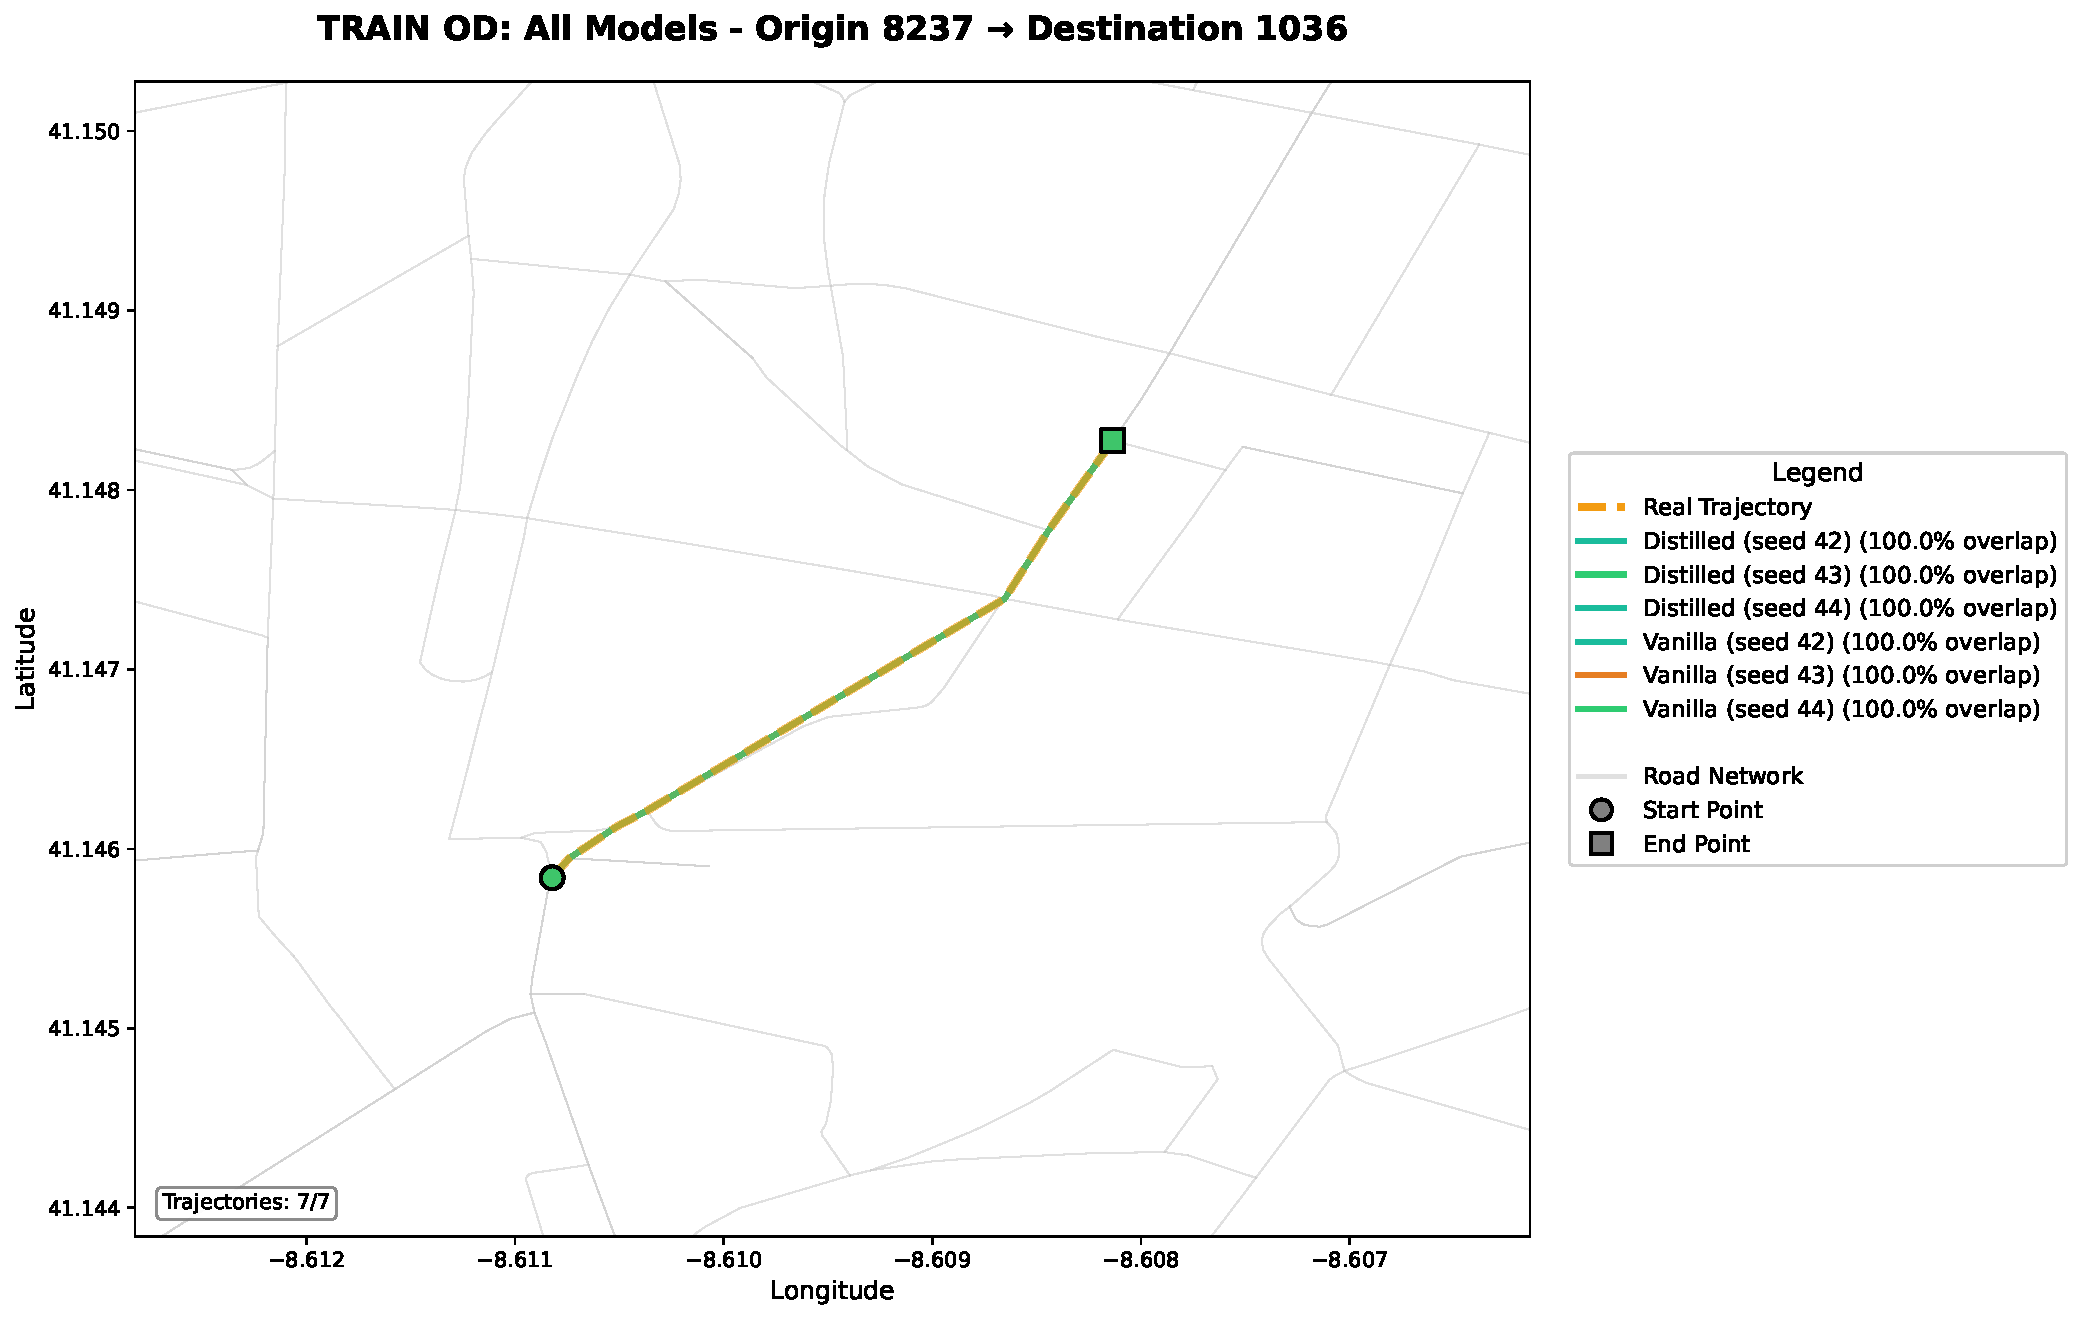
\includegraphics[width=\linewidth]{assets/plots/eval/porto/trajectories/train_od_comparison_1_origin8237_dest1036.pdf}
        \caption{Train OD 1}
    \end{subfigure}
    \begin{subfigure}{0.49\linewidth}
        \centering
        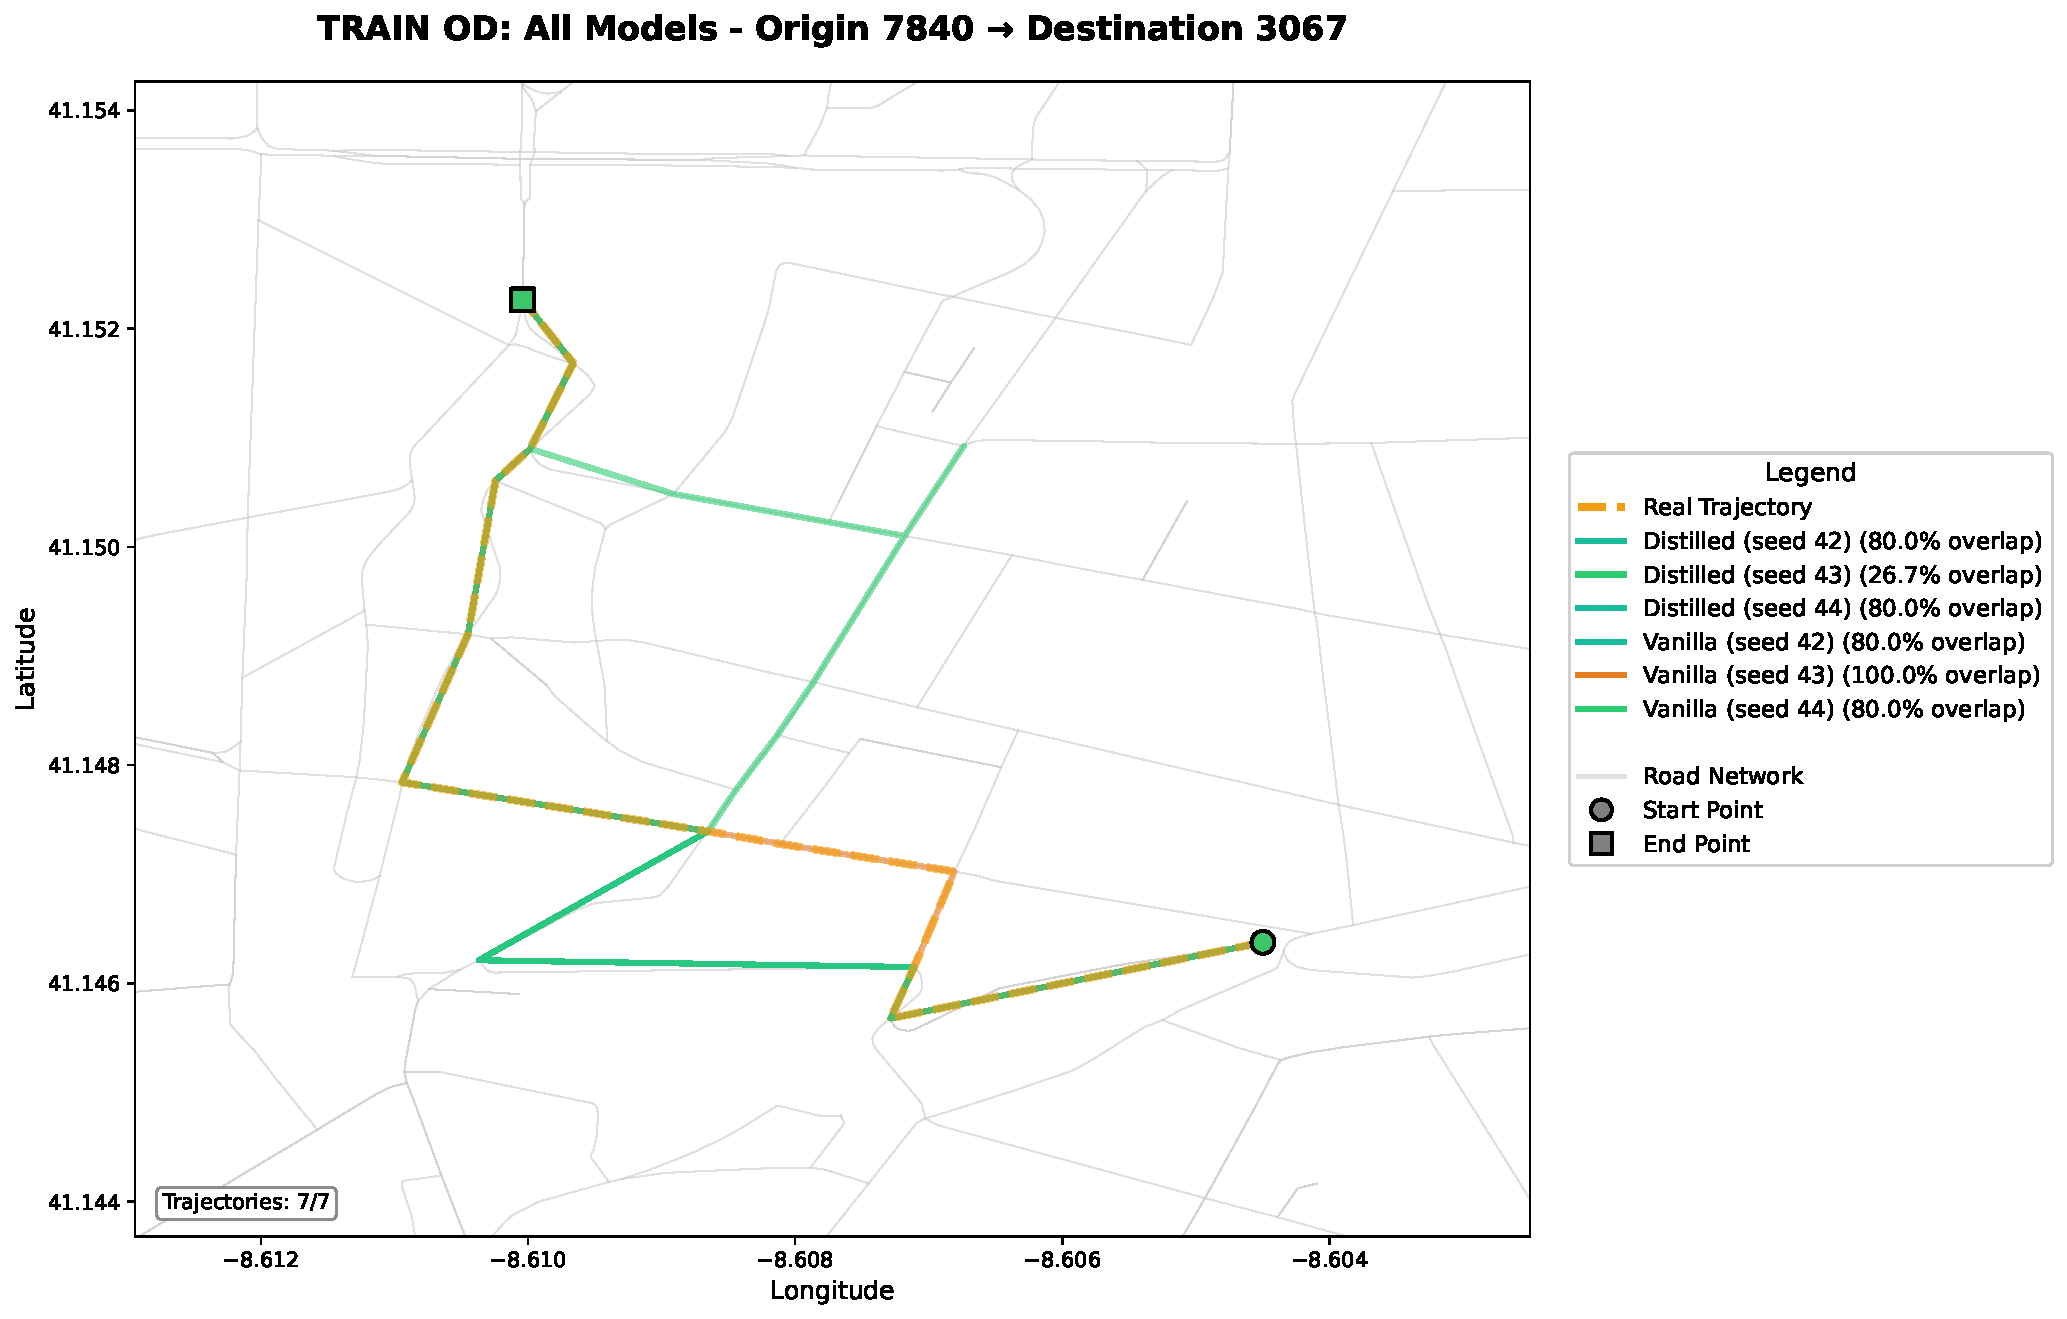
\includegraphics[width=\linewidth]{assets/plots/eval/porto/trajectories/train_od_comparison_3_origin7840_dest3067.pdf}
        \caption{Train OD 3}
    \end{subfigure}
    \begin{subfigure}{0.49\linewidth}
        \centering
        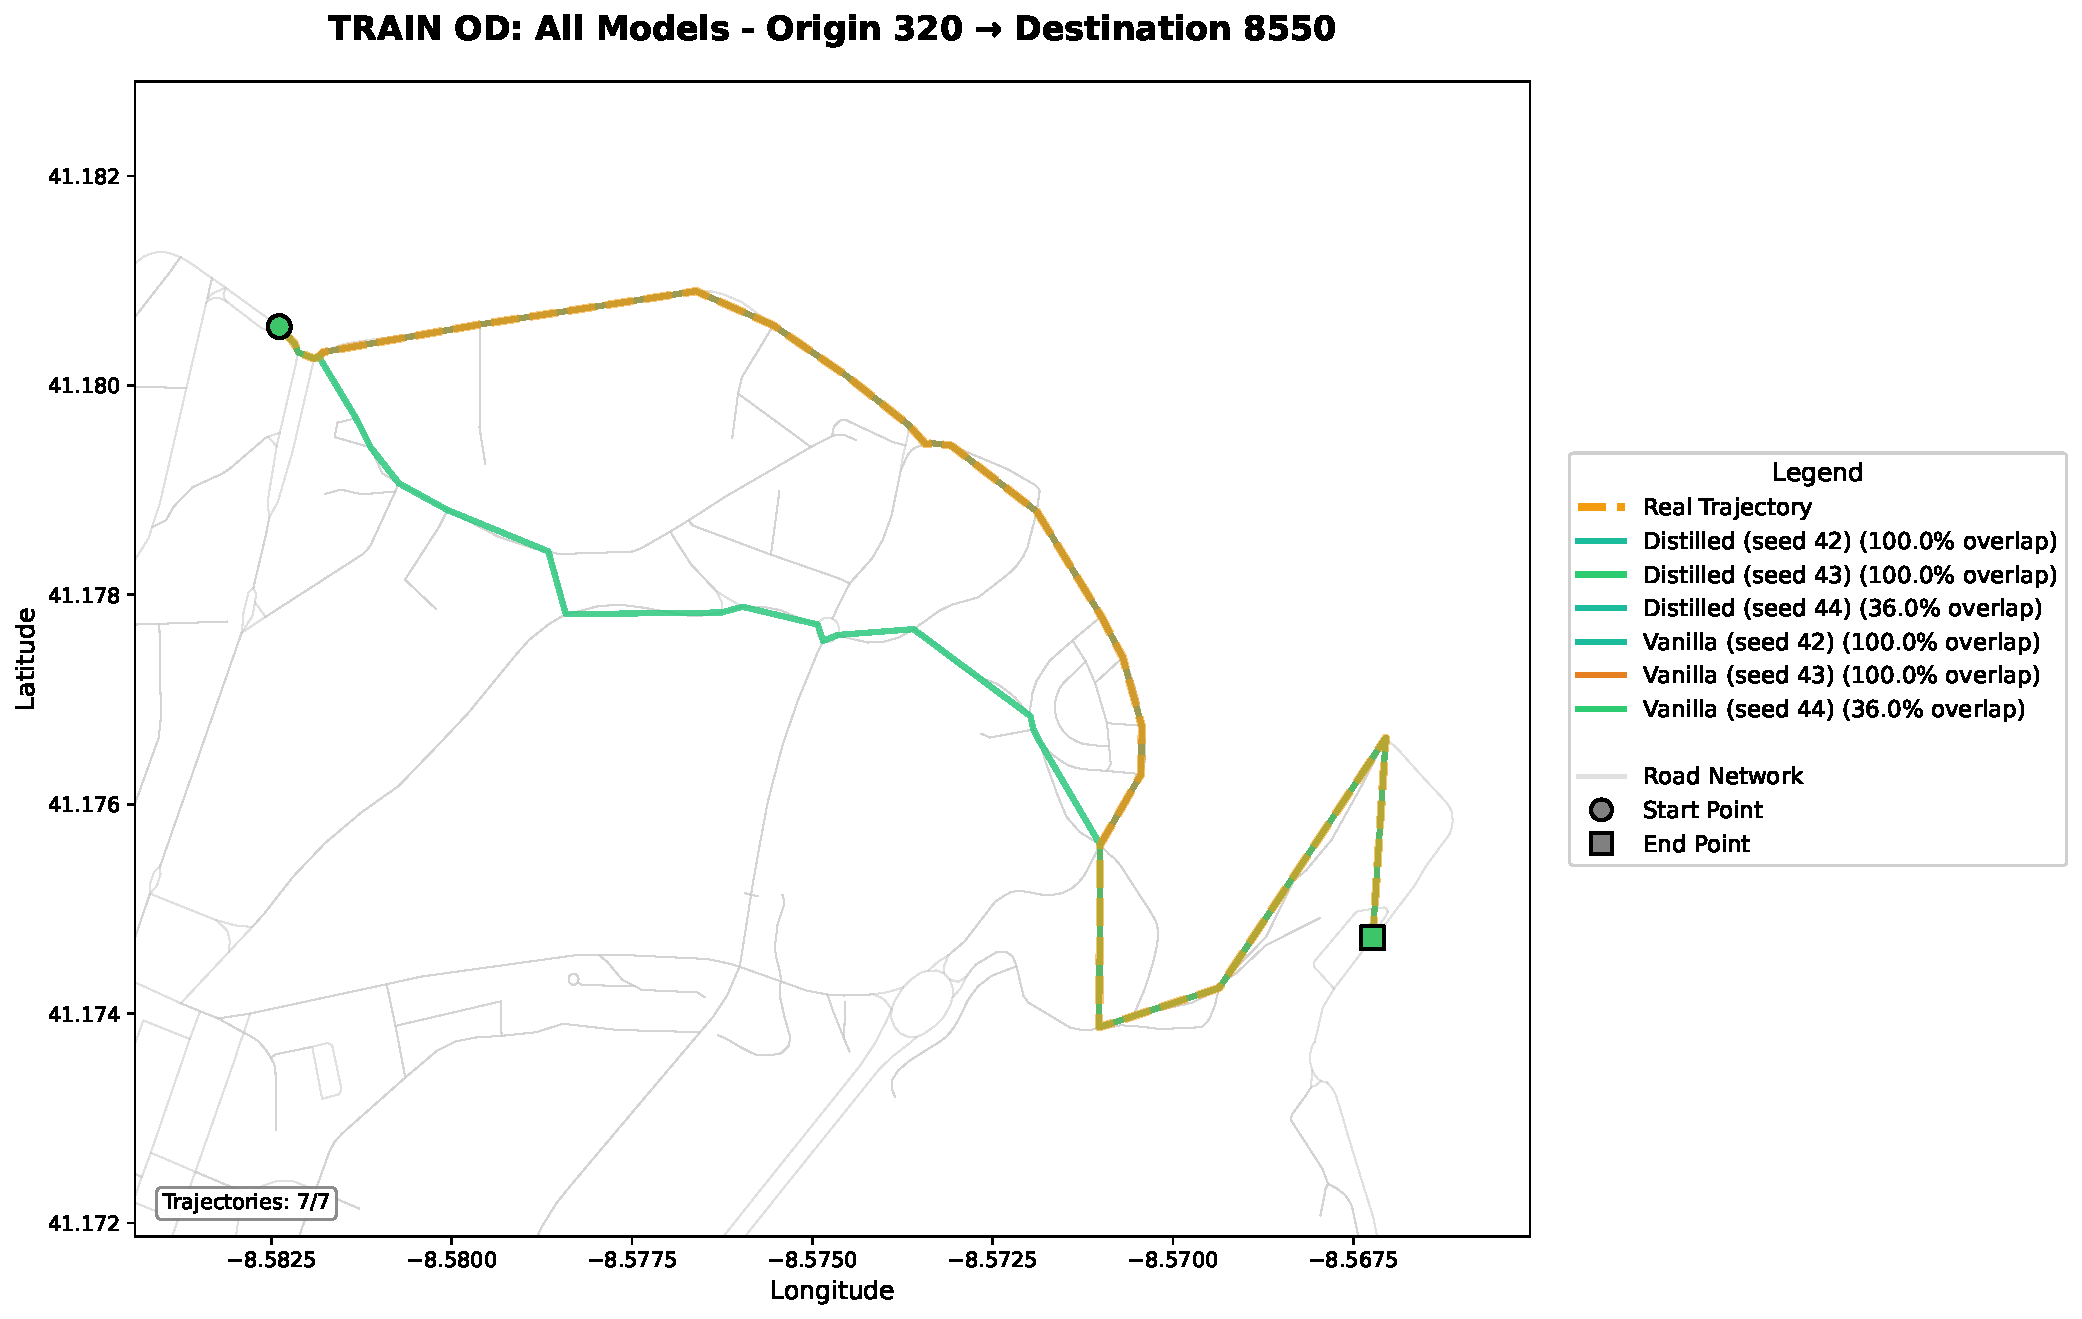
\includegraphics[width=\linewidth]{assets/plots/eval/porto/trajectories/train_od_comparison_5_origin320_dest8550.pdf}
        \caption{Train OD 5}
    \end{subfigure}
    \begin{subfigure}{0.49\linewidth}
        \centering
        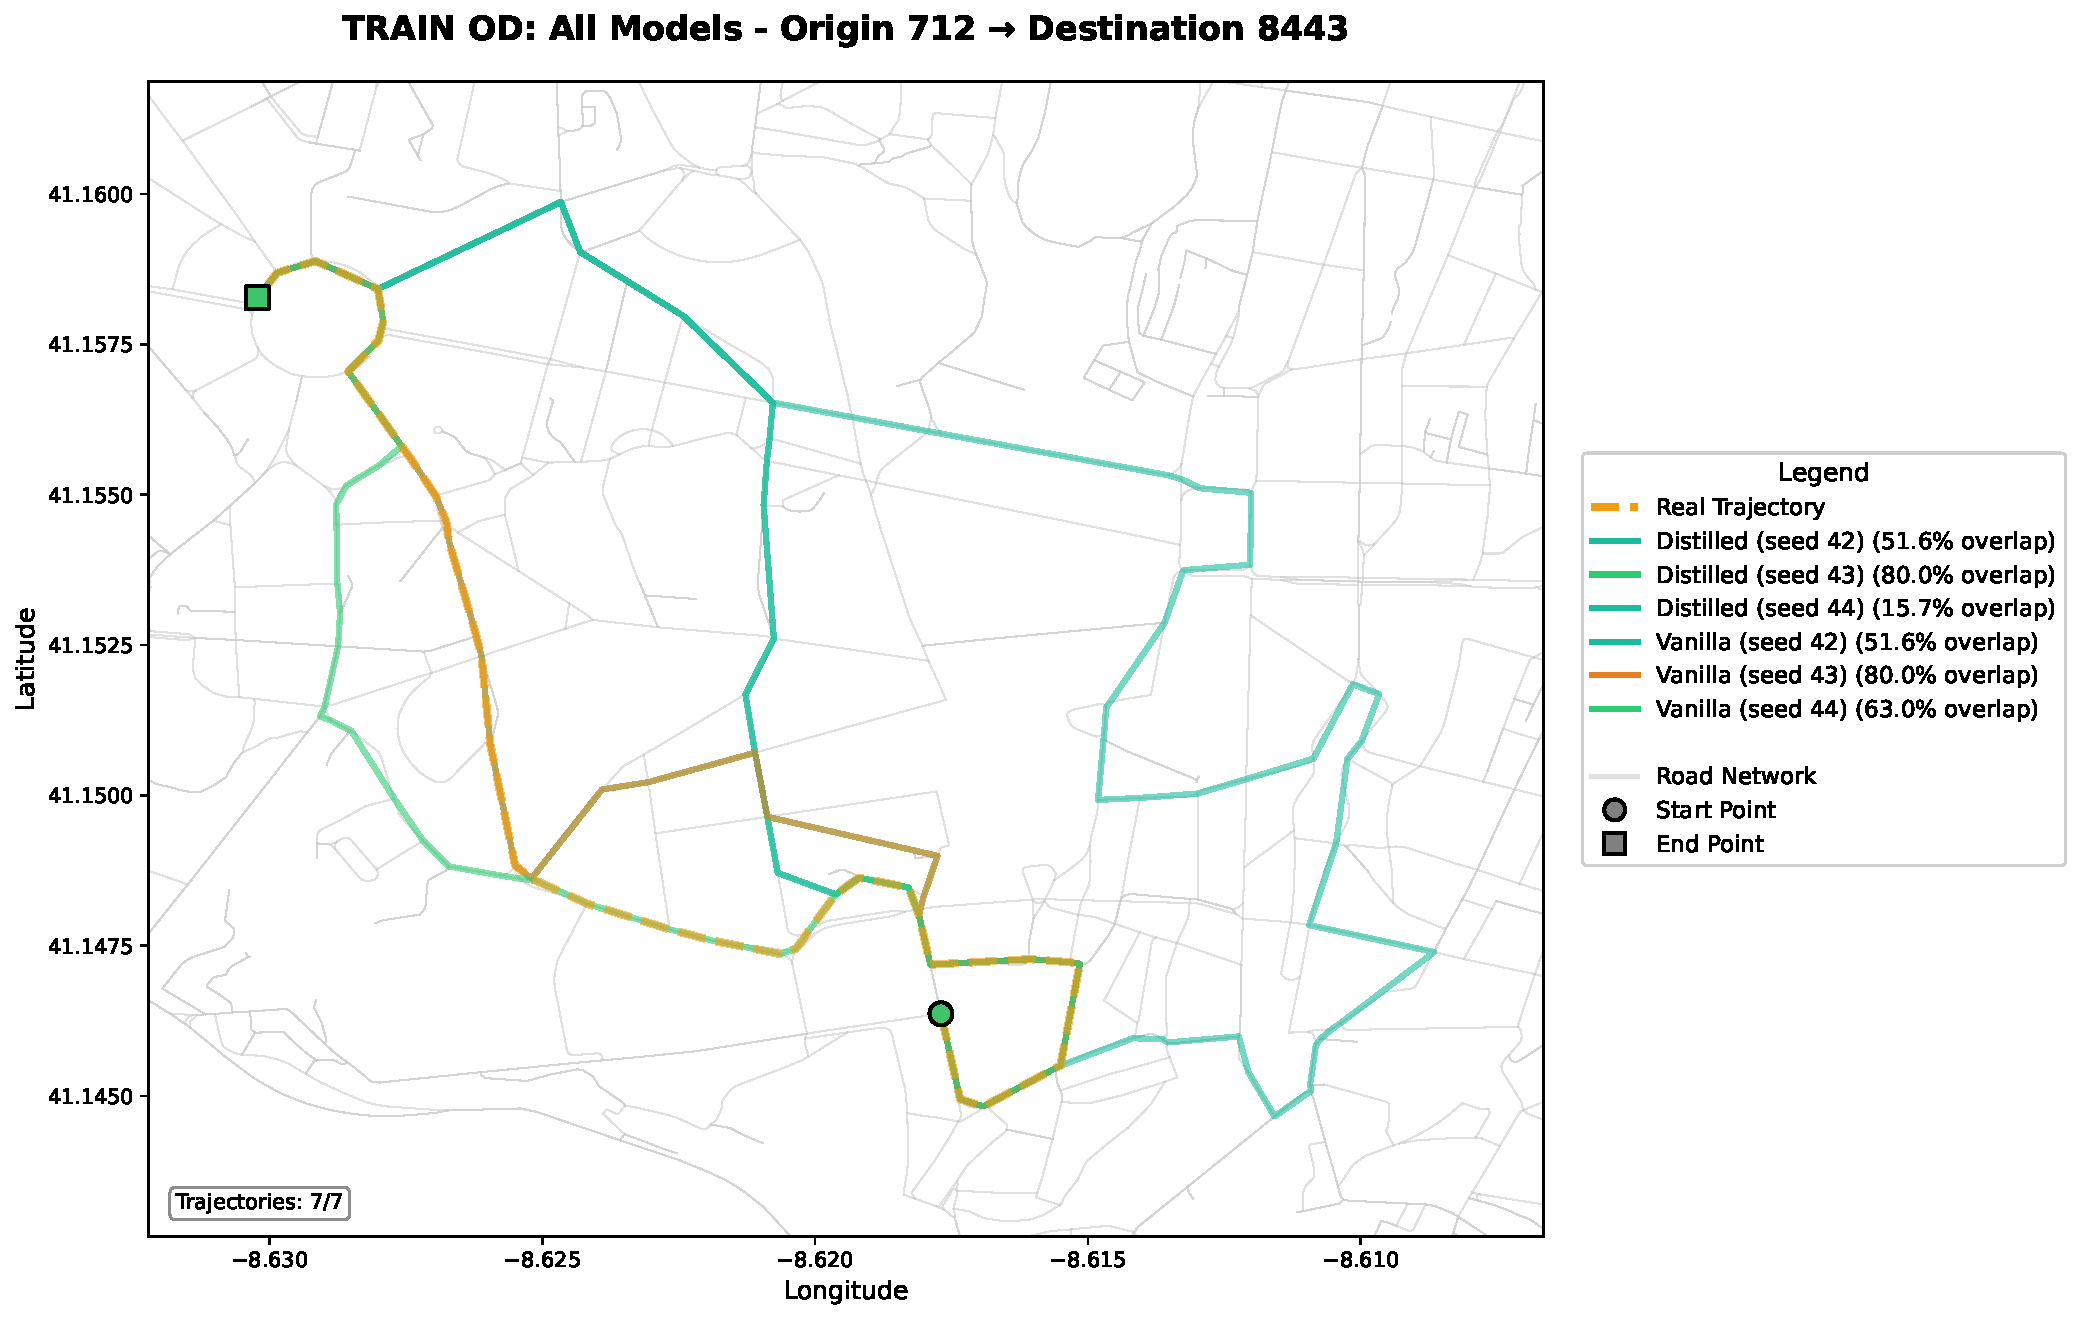
\includegraphics[width=\linewidth]{assets/plots/eval/porto/trajectories/train_od_comparison_7_origin712_dest8443.pdf}
        \caption{Train OD 7}
    \end{subfigure}
    \caption{Porto train OD trajectory examples. Both vanilla and distilled models achieve high path completion rates, with subtle differences in route selection.}
    \label{fig:appendix-porto-traj-train}
\end{figure}

\begin{figure}[H]
    \centering
    \begin{subfigure}{0.49\linewidth}
        \centering
        \includegraphics[width=\linewidth]{assets/plots/eval/porto/trajectories/test_od_comparison_1_origin9991_dest542.pdf}
        \caption{Test OD 1}
    \end{subfigure}
    \begin{subfigure}{0.49\linewidth}
        \centering
        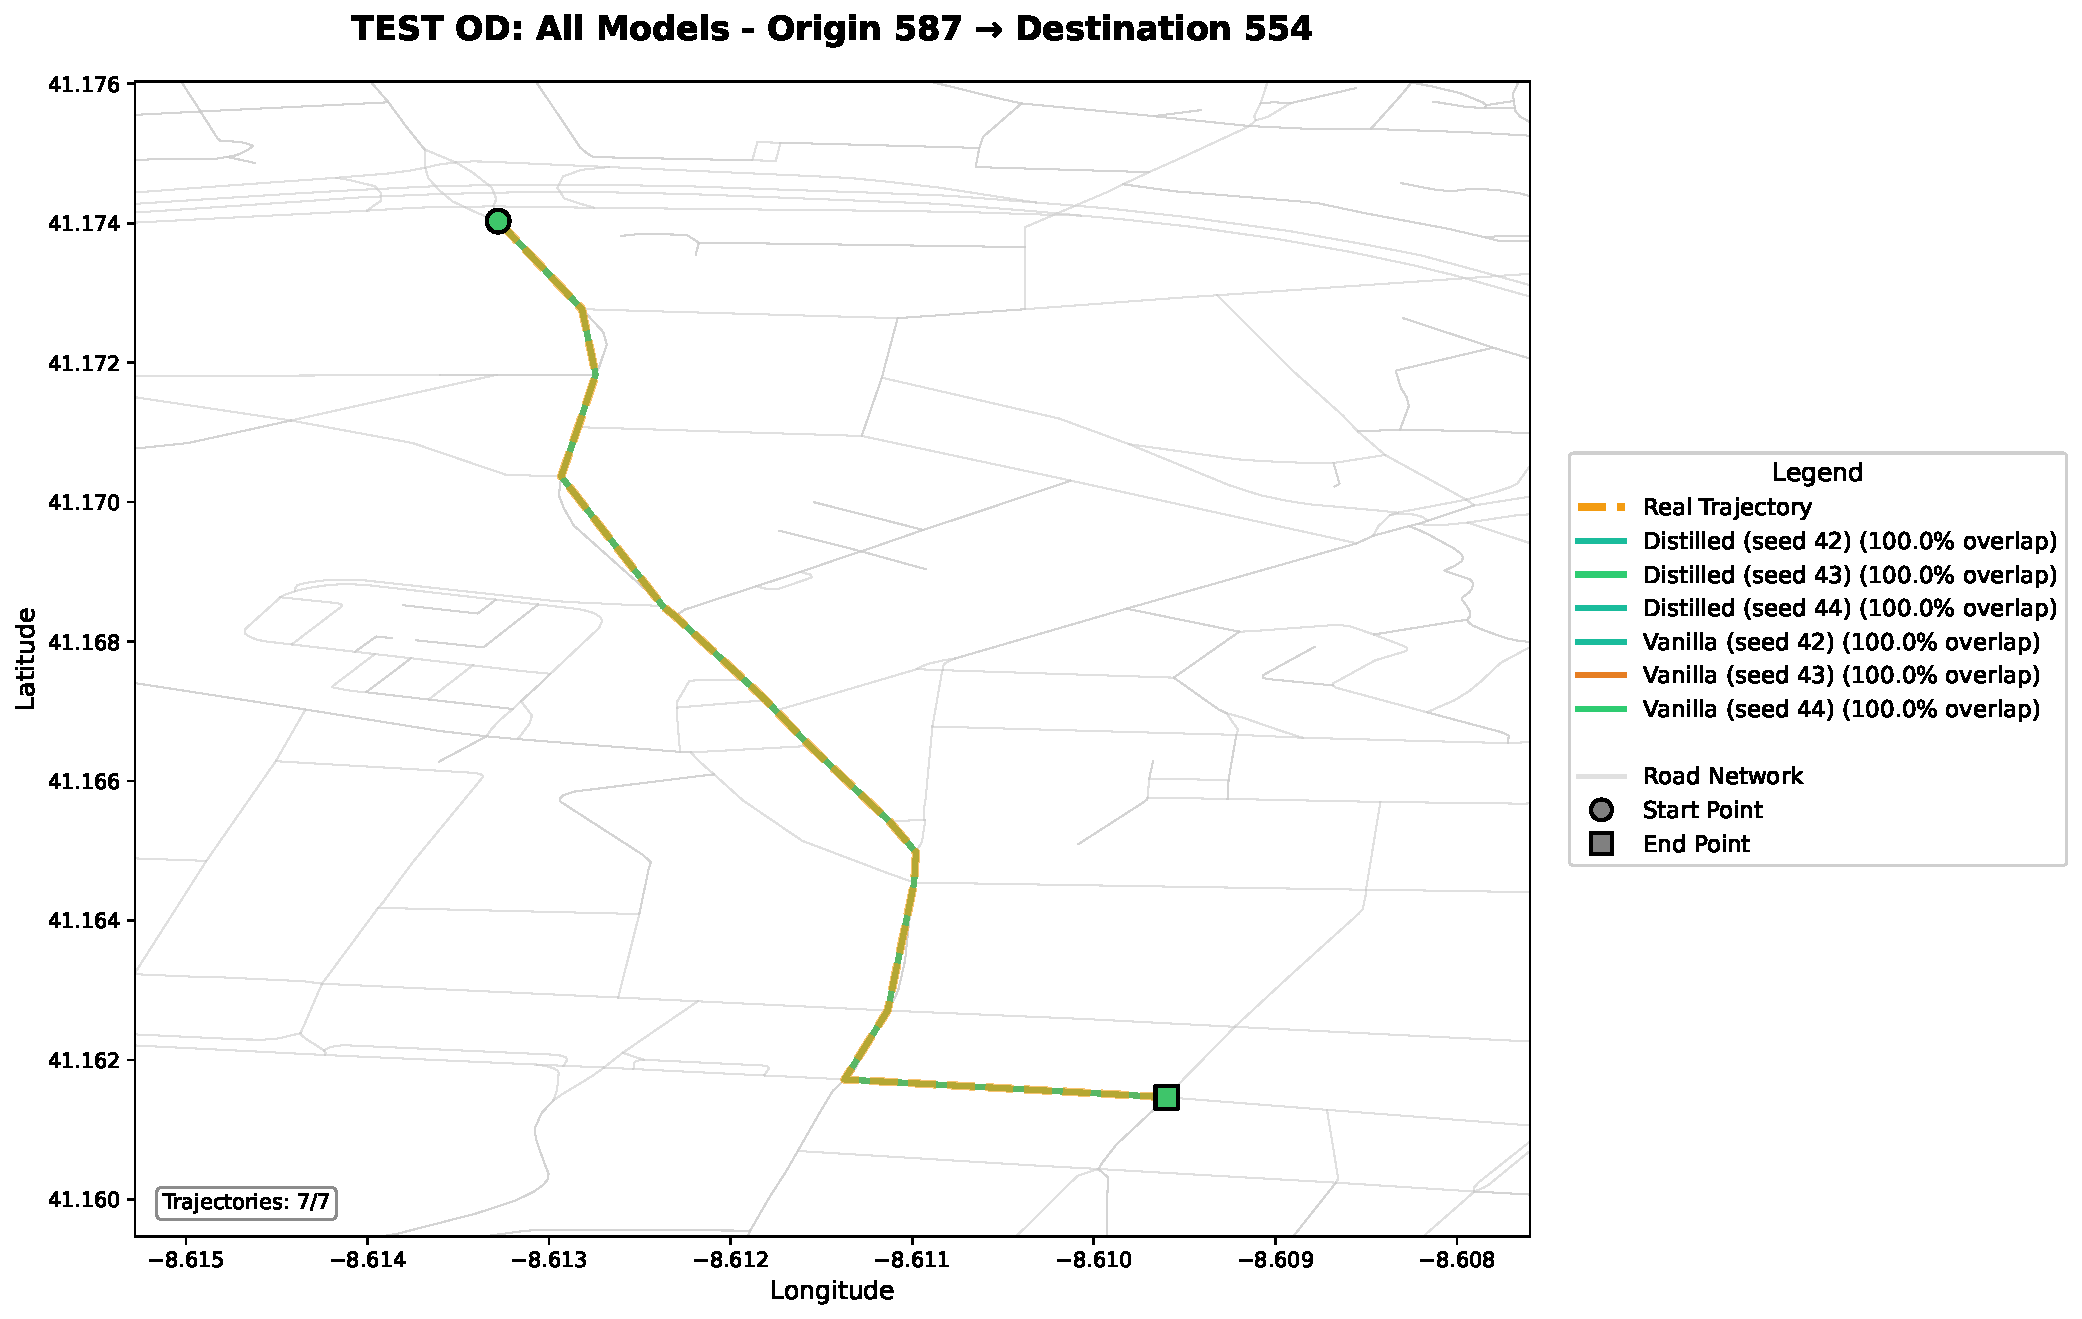
\includegraphics[width=\linewidth]{assets/plots/eval/porto/trajectories/test_od_comparison_3_origin587_dest554.pdf}
        \caption{Test OD 3}
    \end{subfigure}
    \begin{subfigure}{0.49\linewidth}
        \centering
        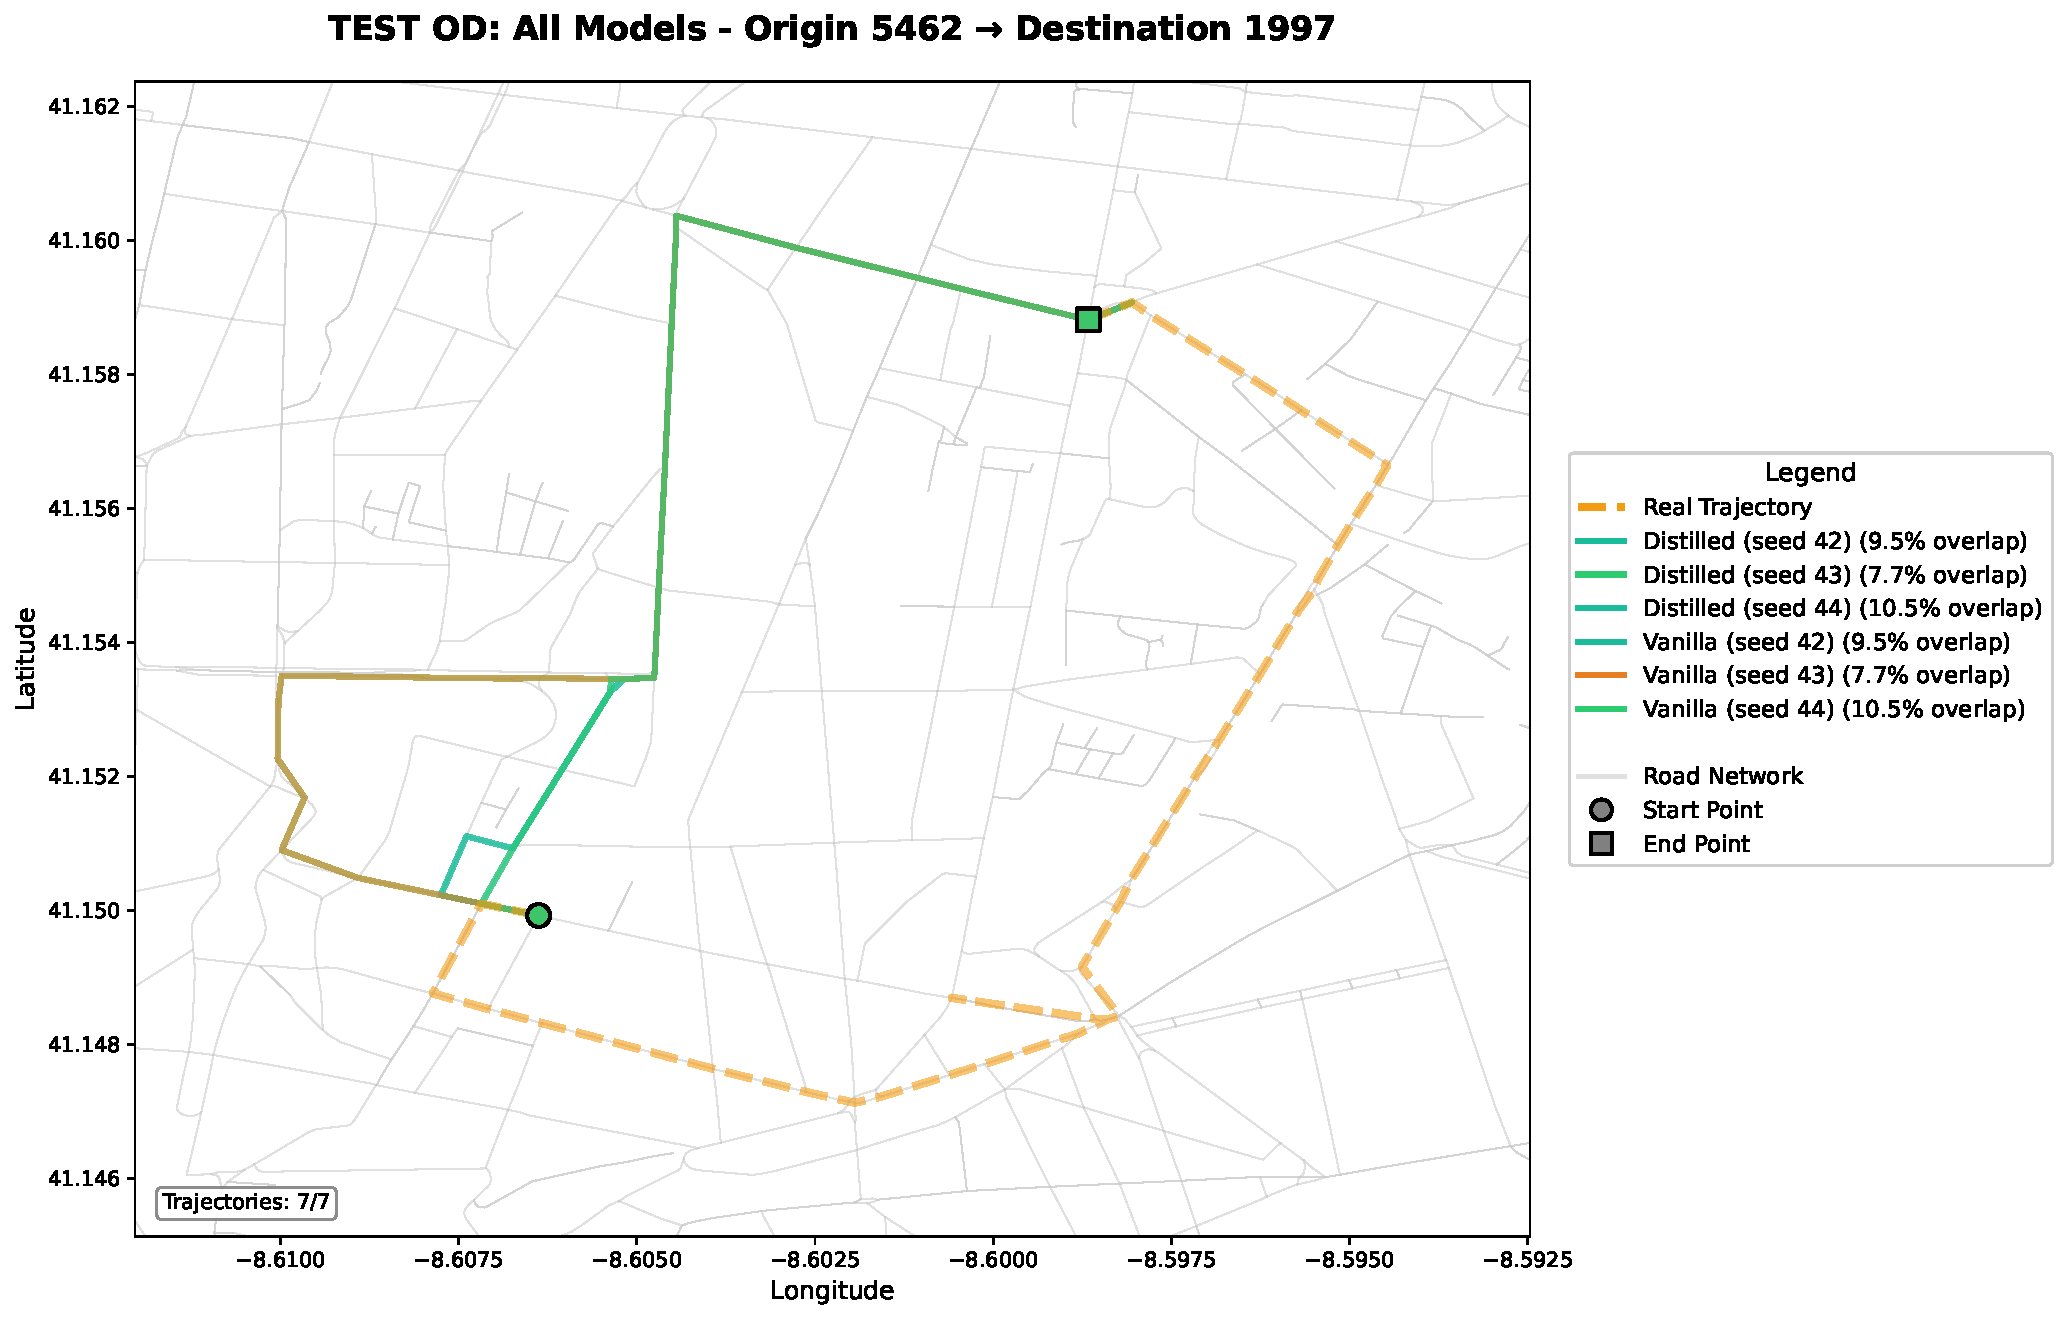
\includegraphics[width=\linewidth]{assets/plots/eval/porto/trajectories/test_od_comparison_5_origin5462_dest1997.pdf}
        \caption{Test OD 5}
    \end{subfigure}
    \begin{subfigure}{0.49\linewidth}
        \centering
        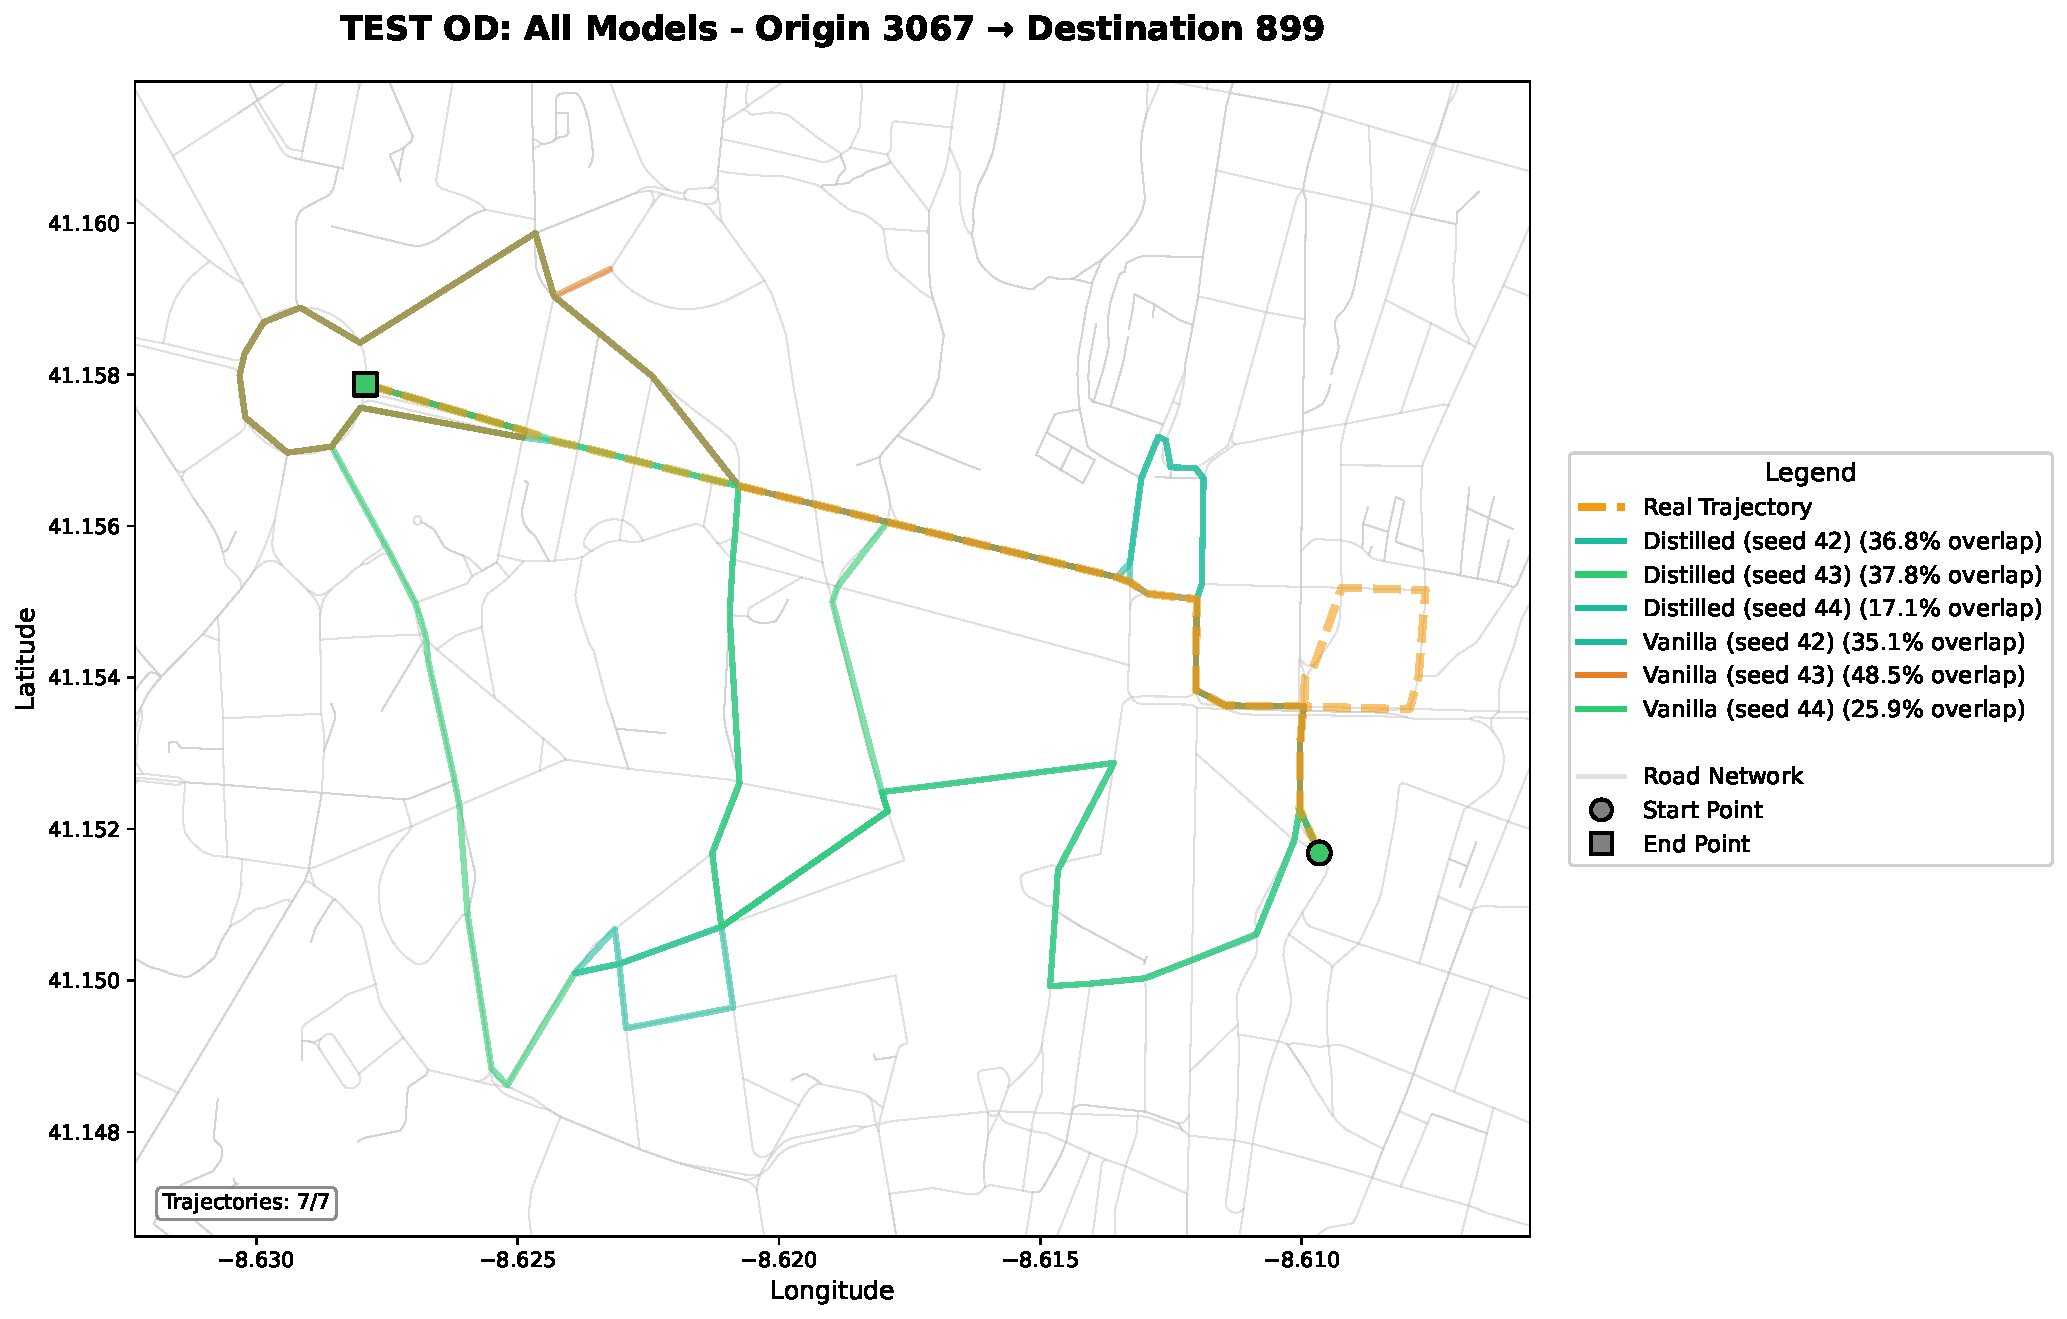
\includegraphics[width=\linewidth]{assets/plots/eval/porto/trajectories/test_od_comparison_7_origin3067_dest899.pdf}
        \caption{Test OD 7}
    \end{subfigure}
    \caption{Porto test OD trajectory examples. Performance on held-out OD pairs demonstrates generalization to new spatial contexts.}
    \label{fig:appendix-porto-traj-test}
\end{figure}

\subsubsection{Cross-Model Trajectory Comparisons (Beijing)}
\label{app:cross-model-beijing}

Figures~\ref{fig:appendix-beijing-cross-test} and~\ref{fig:appendix-beijing-cross-train} present direct side-by-side trajectory visualizations comparing vanilla and distilled model outputs for Beijing, providing qualitative evidence of improved path completion.

\begin{figure}[H]
    \centering
    \begin{subfigure}{0.49\linewidth}
        \centering
        \includegraphics[width=\linewidth]{assets/plots/eval/beijing/cross_model/test_od_comparison_1_origin4462_dest35846.pdf}
        \caption{Test OD 1}
    \end{subfigure}
    \begin{subfigure}{0.49\linewidth}
        \centering
        \includegraphics[width=\linewidth]{assets/plots/eval/beijing/cross_model/test_od_comparison_3_origin24387_dest15499.pdf}
        \caption{Test OD 3}
    \end{subfigure}
    \begin{subfigure}{0.49\linewidth}
        \centering
        \includegraphics[width=\linewidth]{assets/plots/eval/beijing/cross_model/test_od_comparison_5_origin36493_dest3549.pdf}
        \caption{Test OD 5}
    \end{subfigure}
    \begin{subfigure}{0.49\linewidth}
        \centering
        \includegraphics[width=\linewidth]{assets/plots/eval/beijing/cross_model/test_od_comparison_7_origin27117_dest12017.pdf}
        \caption{Test OD 7}
    \end{subfigure}
    \caption{Beijing test OD cross-model comparisons showing vanilla (premature termination) vs distilled (complete paths) behavior.}
    \label{fig:appendix-beijing-cross-test}
\end{figure}

\begin{figure}[H]
    \centering
    \begin{subfigure}{0.49\linewidth}
        \centering
        \includegraphics[width=\linewidth]{assets/plots/eval/beijing/cross_model/train_od_comparison_1_origin32347_dest26801.pdf}
        \caption{Train OD 1}
    \end{subfigure}
    \begin{subfigure}{0.49\linewidth}
        \centering
        \includegraphics[width=\linewidth]{assets/plots/eval/beijing/cross_model/train_od_comparison_3_origin32347_dest37646.pdf}
        \caption{Train OD 3}
    \end{subfigure}
    \begin{subfigure}{0.49\linewidth}
        \centering
        \includegraphics[width=\linewidth]{assets/plots/eval/beijing/cross_model/train_od_comparison_5_origin2466_dest8733.pdf}
        \caption{Train OD 5}
    \end{subfigure}
    \begin{subfigure}{0.49\linewidth}
        \centering
        \includegraphics[width=\linewidth]{assets/plots/eval/beijing/cross_model/train_od_comparison_7_origin20252_dest22542.pdf}
        \caption{Train OD 7}
    \end{subfigure}
    \caption{Beijing train OD cross-model comparisons demonstrating consistent distillation improvements even on training set OD pairs.}
    \label{fig:appendix-beijing-cross-train}
\end{figure}

\paragraph{Scenario-Specific Cross-Model Comparisons (Beijing)}

Figure~\ref{fig:appendix-beijing-scenario-city-center} presents scenario-specific cross-model trajectory comparisons for Beijing, showing the dramatic improvement from distillation across spatial contexts.

\begin{figure}[H]
    \centering
    \begin{subfigure}{0.8\linewidth}
        \centering
        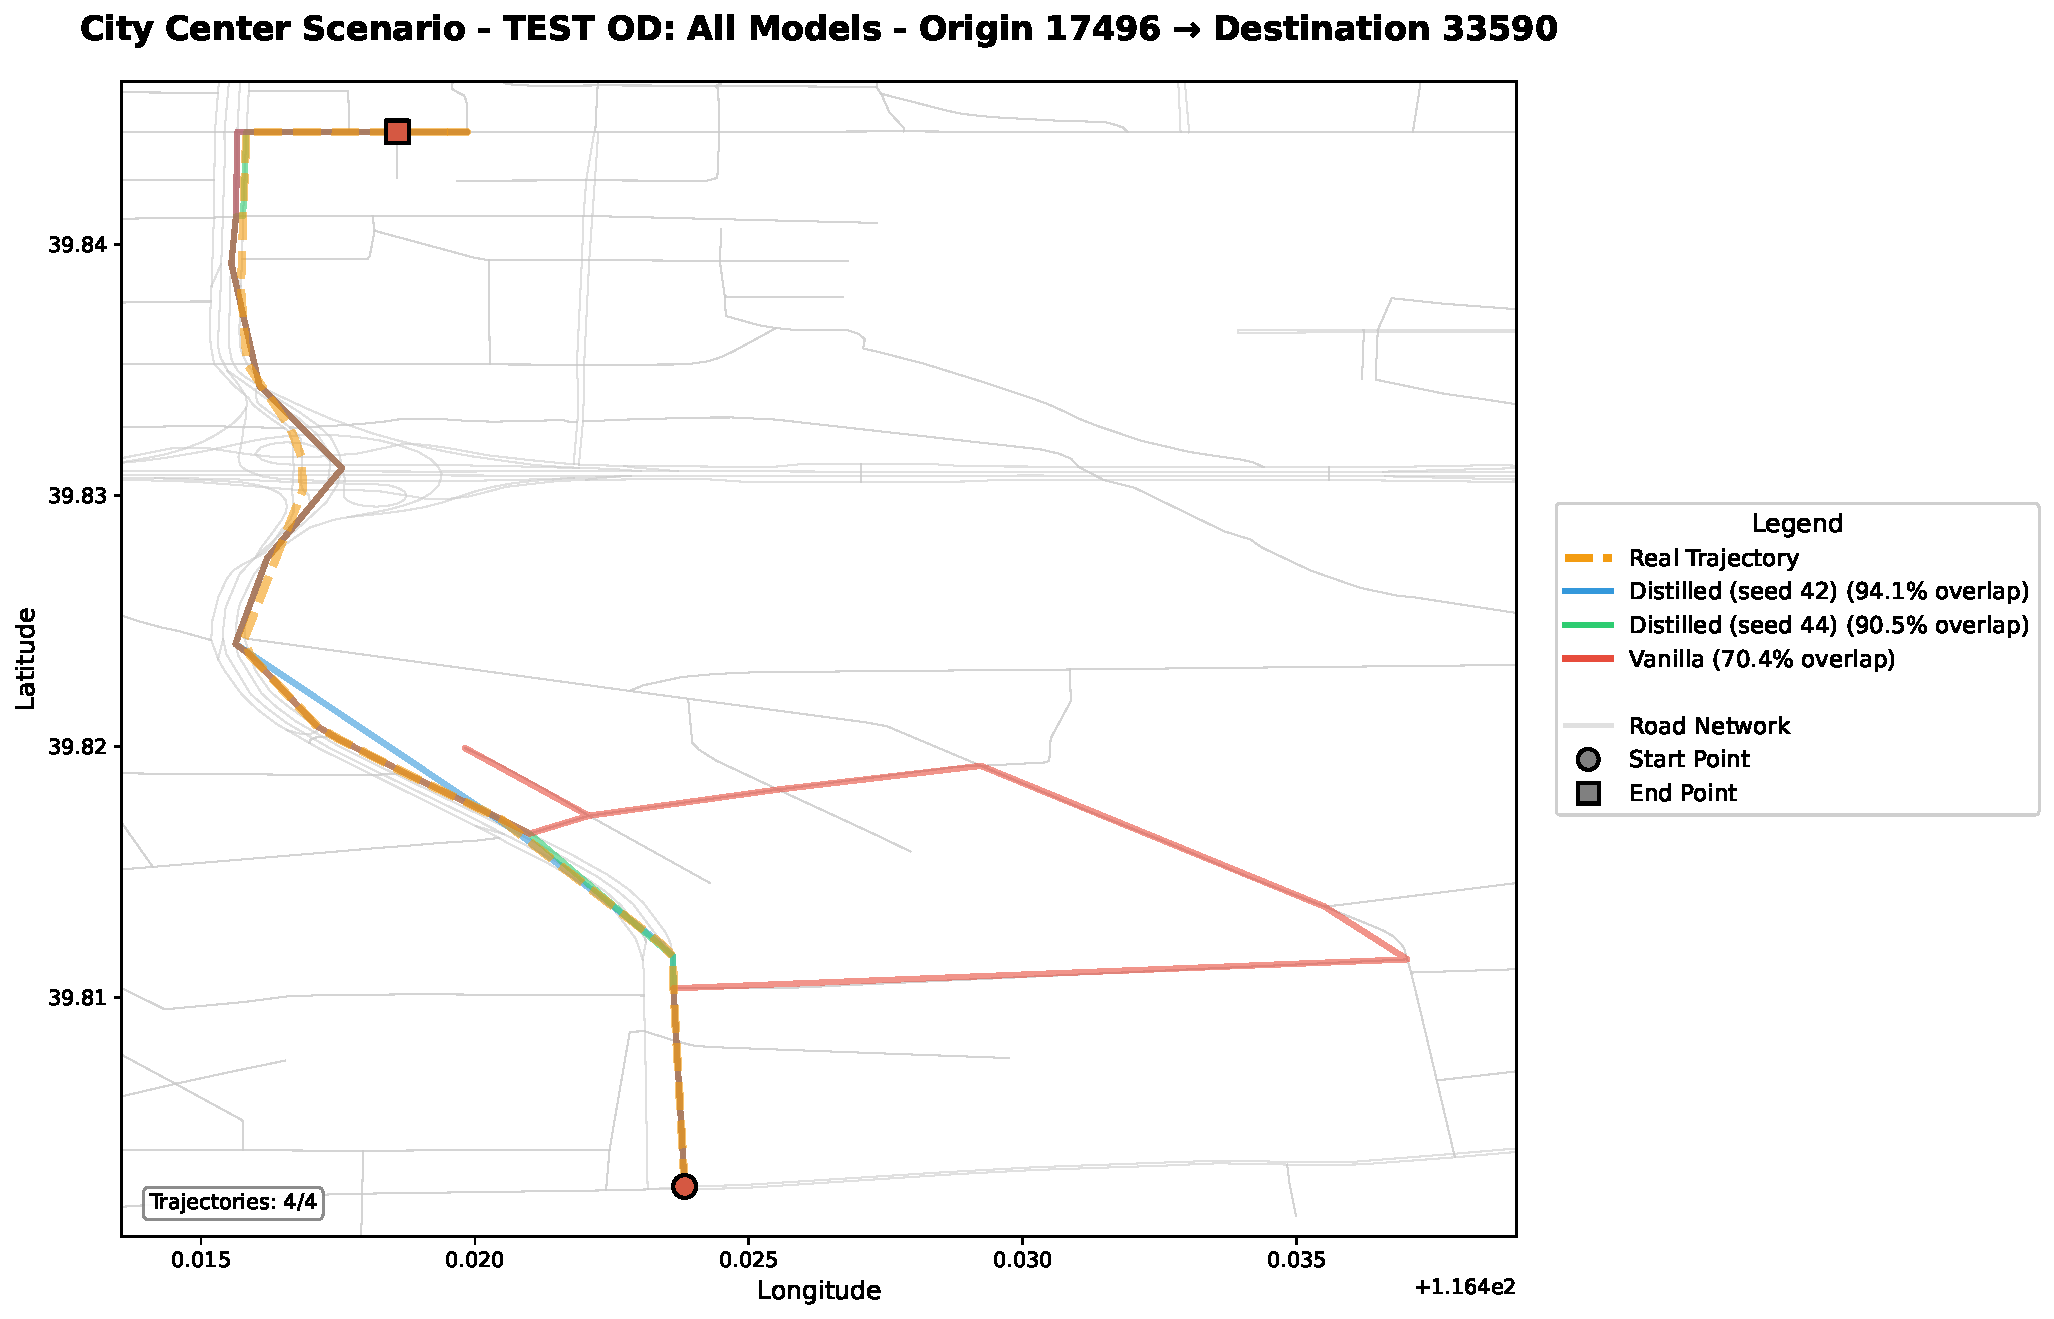
\includegraphics[width=\linewidth]{assets/plots/eval/beijing/scenario_cross_model/test/city_center/test_od_comparison_1_origin17496_dest33590.pdf}
        \caption{City center: Test OD comparison showing vanilla premature termination vs distilled complete path}
    \end{subfigure}
    \caption{Beijing city center scenario cross-model comparison. Demonstrates universal distillation benefit characteristic of Beijing, where teacher knowledge dramatically improves path completion regardless of spatial context.}
    \label{fig:appendix-beijing-scenario-city-center}
\end{figure}

\subsubsection{Cross-Model Trajectory Comparisons (Porto)}
\label{app:cross-model-porto}

Figures~\ref{fig:appendix-porto-cross-test} through~\ref{fig:appendix-porto-scenario-suburban} present direct side-by-side trajectory visualizations for Porto, showing subtle differences in route selection and distribution quality. Additionally, Figures~\ref{fig:appendix-porto-scenario-city-center} and~\ref{fig:appendix-porto-scenario-suburban} show scenario-specific comparisons revealing context-dependent performance patterns.

\begin{figure}[H]
    \centering
    \begin{subfigure}{0.49\linewidth}
        \centering
        \includegraphics[width=\linewidth]{assets/plots/eval/porto/cross_model/test/test_od_comparison_1_origin9991_dest542.pdf}
        \caption{Test OD 1}
    \end{subfigure}
    \begin{subfigure}{0.49\linewidth}
        \centering
        \includegraphics[width=\linewidth]{assets/plots/eval/porto/cross_model/test/test_od_comparison_3_origin587_dest554.pdf}
        \caption{Test OD 3}
    \end{subfigure}
    \begin{subfigure}{0.49\linewidth}
        \centering
        \includegraphics[width=\linewidth]{assets/plots/eval/porto/cross_model/test/test_od_comparison_5_origin5462_dest1997.pdf}
        \caption{Test OD 5}
    \end{subfigure}
    \begin{subfigure}{0.49\linewidth}
        \centering
        \includegraphics[width=\linewidth]{assets/plots/eval/porto/cross_model/test/test_od_comparison_7_origin3067_dest899.pdf}
        \caption{Test OD 7}
    \end{subfigure}
    \caption{Porto test OD cross-model comparisons. Both models complete most paths; differences appear in route choice and spatial distribution.}
    \label{fig:appendix-porto-cross-test}
\end{figure}

\begin{figure}[H]
    \centering
    \begin{subfigure}{0.49\linewidth}
        \centering
        \includegraphics[width=\linewidth]{assets/plots/eval/porto/cross_model/train/train_od_comparison_1_origin8237_dest1036.pdf}
        \caption{Train OD 1}
    \end{subfigure}
    \begin{subfigure}{0.49\linewidth}
        \centering
        \includegraphics[width=\linewidth]{assets/plots/eval/porto/cross_model/train/train_od_comparison_3_origin7840_dest3067.pdf}
        \caption{Train OD 3}
    \end{subfigure}
    \begin{subfigure}{0.49\linewidth}
        \centering
        \includegraphics[width=\linewidth]{assets/plots/eval/porto/cross_model/train/train_od_comparison_5_origin320_dest8550.pdf}
        \caption{Train OD 5}
    \end{subfigure}
    \begin{subfigure}{0.49\linewidth}
        \centering
        \includegraphics[width=\linewidth]{assets/plots/eval/porto/cross_model/train/train_od_comparison_7_origin712_dest8443.pdf}
        \caption{Train OD 7}
    \end{subfigure}
    \caption{Porto train OD cross-model comparisons showing baseline high performance with marginal distillation improvements.}
    \label{fig:appendix-porto-cross-train}
\end{figure}

\paragraph{Scenario-Specific Cross-Model Comparisons (Porto)}

Figures~\ref{fig:appendix-porto-scenario-city-center} and~\ref{fig:appendix-porto-scenario-suburban} present cross-model trajectory comparisons for specific spatial scenarios, demonstrating how distillation benefits vary by urban context in Porto (contrasting with Beijing's universal improvements shown in Figure~\ref{fig:appendix-beijing-scenario-city-center}). City center trajectories show where teacher knowledge provides spatial guidance, while suburban trajectories reveal contexts where vanilla models already perform well.

\begin{figure}[H]
    \centering
    \begin{subfigure}{0.49\linewidth}
        \centering
        \includegraphics[width=\linewidth]{assets/plots/eval/porto/scenario_cross_model/test/city_center/test_od_comparison_1_origin234_dest7406.pdf}
        \caption{City center: Test OD 1}
    \end{subfigure}
    \begin{subfigure}{0.49\linewidth}
        \centering
        \includegraphics[width=\linewidth]{assets/plots/eval/porto/scenario_cross_model/test/city_center/test_od_comparison_3_origin587_dest554.pdf}
        \caption{City center: Test OD 3}
    \end{subfigure}
    \begin{subfigure}{0.49\linewidth}
        \centering
        \includegraphics[width=\linewidth]{assets/plots/eval/porto/scenario_cross_model/train/city_center/train_od_comparison_1_origin8435_dest357.pdf}
        \caption{City center: Train OD 1}
    \end{subfigure}
    \begin{subfigure}{0.49\linewidth}
        \centering
        \includegraphics[width=\linewidth]{assets/plots/eval/porto/scenario_cross_model/train/city_center/train_od_comparison_3_origin10016_dest1949.pdf}
        \caption{City center: Train OD 3}
    \end{subfigure}
    \caption{Porto city center scenario cross-model comparisons. Dense urban context where distillation provides spatial guidance benefits, reflecting teacher (LM-TAD) training domain expertise.}
    \label{fig:appendix-porto-scenario-city-center}
\end{figure}

\begin{figure}[H]
    \centering
    \begin{subfigure}{0.8\linewidth}
        \centering
        \includegraphics[width=\linewidth]{assets/plots/eval/porto/scenario_cross_model/test/suburban/test_od_comparison_1_origin10232_dest2811.pdf}
        \caption{Suburban: Test OD comparison (only one suitable pair found for this scenario)}
    \end{subfigure}
    \caption{Porto suburban scenario cross-model comparison. Lower-density context where vanilla already performs well, showing limited marginal benefit from distillation. Demonstrates spatial localization of teacher knowledge.}
    \label{fig:appendix-porto-scenario-suburban}
\end{figure}


\end{document}